% Options for packages loaded elsewhere
\PassOptionsToPackage{unicode}{hyperref}
\PassOptionsToPackage{hyphens}{url}
%
\documentclass[
]{book}
\usepackage{amsmath,amssymb}
\usepackage{iftex}
\ifPDFTeX
  \usepackage[T1]{fontenc}
  \usepackage[utf8]{inputenc}
  \usepackage{textcomp} % provide euro and other symbols
\else % if luatex or xetex
  \usepackage{unicode-math} % this also loads fontspec
  \defaultfontfeatures{Scale=MatchLowercase}
  \defaultfontfeatures[\rmfamily]{Ligatures=TeX,Scale=1}
\fi
\usepackage{lmodern}
\ifPDFTeX\else
  % xetex/luatex font selection
\fi
% Use upquote if available, for straight quotes in verbatim environments
\IfFileExists{upquote.sty}{\usepackage{upquote}}{}
\IfFileExists{microtype.sty}{% use microtype if available
  \usepackage[]{microtype}
  \UseMicrotypeSet[protrusion]{basicmath} % disable protrusion for tt fonts
}{}
\makeatletter
\@ifundefined{KOMAClassName}{% if non-KOMA class
  \IfFileExists{parskip.sty}{%
    \usepackage{parskip}
  }{% else
    \setlength{\parindent}{0pt}
    \setlength{\parskip}{6pt plus 2pt minus 1pt}}
}{% if KOMA class
  \KOMAoptions{parskip=half}}
\makeatother
\usepackage{xcolor}
\usepackage{color}
\usepackage{fancyvrb}
\newcommand{\VerbBar}{|}
\newcommand{\VERB}{\Verb[commandchars=\\\{\}]}
\DefineVerbatimEnvironment{Highlighting}{Verbatim}{commandchars=\\\{\}}
% Add ',fontsize=\small' for more characters per line
\usepackage{framed}
\definecolor{shadecolor}{RGB}{248,248,248}
\newenvironment{Shaded}{\begin{snugshade}}{\end{snugshade}}
\newcommand{\AlertTok}[1]{\textcolor[rgb]{0.94,0.16,0.16}{#1}}
\newcommand{\AnnotationTok}[1]{\textcolor[rgb]{0.56,0.35,0.01}{\textbf{\textit{#1}}}}
\newcommand{\AttributeTok}[1]{\textcolor[rgb]{0.13,0.29,0.53}{#1}}
\newcommand{\BaseNTok}[1]{\textcolor[rgb]{0.00,0.00,0.81}{#1}}
\newcommand{\BuiltInTok}[1]{#1}
\newcommand{\CharTok}[1]{\textcolor[rgb]{0.31,0.60,0.02}{#1}}
\newcommand{\CommentTok}[1]{\textcolor[rgb]{0.56,0.35,0.01}{\textit{#1}}}
\newcommand{\CommentVarTok}[1]{\textcolor[rgb]{0.56,0.35,0.01}{\textbf{\textit{#1}}}}
\newcommand{\ConstantTok}[1]{\textcolor[rgb]{0.56,0.35,0.01}{#1}}
\newcommand{\ControlFlowTok}[1]{\textcolor[rgb]{0.13,0.29,0.53}{\textbf{#1}}}
\newcommand{\DataTypeTok}[1]{\textcolor[rgb]{0.13,0.29,0.53}{#1}}
\newcommand{\DecValTok}[1]{\textcolor[rgb]{0.00,0.00,0.81}{#1}}
\newcommand{\DocumentationTok}[1]{\textcolor[rgb]{0.56,0.35,0.01}{\textbf{\textit{#1}}}}
\newcommand{\ErrorTok}[1]{\textcolor[rgb]{0.64,0.00,0.00}{\textbf{#1}}}
\newcommand{\ExtensionTok}[1]{#1}
\newcommand{\FloatTok}[1]{\textcolor[rgb]{0.00,0.00,0.81}{#1}}
\newcommand{\FunctionTok}[1]{\textcolor[rgb]{0.13,0.29,0.53}{\textbf{#1}}}
\newcommand{\ImportTok}[1]{#1}
\newcommand{\InformationTok}[1]{\textcolor[rgb]{0.56,0.35,0.01}{\textbf{\textit{#1}}}}
\newcommand{\KeywordTok}[1]{\textcolor[rgb]{0.13,0.29,0.53}{\textbf{#1}}}
\newcommand{\NormalTok}[1]{#1}
\newcommand{\OperatorTok}[1]{\textcolor[rgb]{0.81,0.36,0.00}{\textbf{#1}}}
\newcommand{\OtherTok}[1]{\textcolor[rgb]{0.56,0.35,0.01}{#1}}
\newcommand{\PreprocessorTok}[1]{\textcolor[rgb]{0.56,0.35,0.01}{\textit{#1}}}
\newcommand{\RegionMarkerTok}[1]{#1}
\newcommand{\SpecialCharTok}[1]{\textcolor[rgb]{0.81,0.36,0.00}{\textbf{#1}}}
\newcommand{\SpecialStringTok}[1]{\textcolor[rgb]{0.31,0.60,0.02}{#1}}
\newcommand{\StringTok}[1]{\textcolor[rgb]{0.31,0.60,0.02}{#1}}
\newcommand{\VariableTok}[1]{\textcolor[rgb]{0.00,0.00,0.00}{#1}}
\newcommand{\VerbatimStringTok}[1]{\textcolor[rgb]{0.31,0.60,0.02}{#1}}
\newcommand{\WarningTok}[1]{\textcolor[rgb]{0.56,0.35,0.01}{\textbf{\textit{#1}}}}
\usepackage{longtable,booktabs,array}
\usepackage{calc} % for calculating minipage widths
% Correct order of tables after \paragraph or \subparagraph
\usepackage{etoolbox}
\makeatletter
\patchcmd\longtable{\par}{\if@noskipsec\mbox{}\fi\par}{}{}
\makeatother
% Allow footnotes in longtable head/foot
\IfFileExists{footnotehyper.sty}{\usepackage{footnotehyper}}{\usepackage{footnote}}
\makesavenoteenv{longtable}
\usepackage{graphicx}
\makeatletter
\def\maxwidth{\ifdim\Gin@nat@width>\linewidth\linewidth\else\Gin@nat@width\fi}
\def\maxheight{\ifdim\Gin@nat@height>\textheight\textheight\else\Gin@nat@height\fi}
\makeatother
% Scale images if necessary, so that they will not overflow the page
% margins by default, and it is still possible to overwrite the defaults
% using explicit options in \includegraphics[width, height, ...]{}
\setkeys{Gin}{width=\maxwidth,height=\maxheight,keepaspectratio}
% Set default figure placement to htbp
\makeatletter
\def\fps@figure{htbp}
\makeatother
\setlength{\emergencystretch}{3em} % prevent overfull lines
\providecommand{\tightlist}{%
  \setlength{\itemsep}{0pt}\setlength{\parskip}{0pt}}
\setcounter{secnumdepth}{5}
\usepackage{booktabs}
\ifLuaTeX
  \usepackage{selnolig}  % disable illegal ligatures
\fi
\usepackage[]{natbib}
\bibliographystyle{plainnat}
\IfFileExists{bookmark.sty}{\usepackage{bookmark}}{\usepackage{hyperref}}
\IfFileExists{xurl.sty}{\usepackage{xurl}}{} % add URL line breaks if available
\urlstyle{same}
\hypersetup{
  pdftitle={Web Technologies in R},
  pdfauthor={Gaston Sanchez},
  hidelinks,
  pdfcreator={LaTeX via pandoc}}

\title{Web Technologies in R}
\usepackage{etoolbox}
\makeatletter
\providecommand{\subtitle}[1]{% add subtitle to \maketitle
  \apptocmd{\@title}{\par {\large #1 \par}}{}{}
}
\makeatother
\subtitle{A Short Introduction to Web Technologies in R}
\author{Gaston Sanchez}
\date{November 2022}

\begin{document}
\maketitle

{
\setcounter{tocdepth}{1}
\tableofcontents
}
\hypertarget{about}{%
\chapter*{About}\label{about}}
\addcontentsline{toc}{chapter}{About}

In this manuscript I provide an overview of some of the Web Technologies
available in R.

\hypertarget{about-you}{%
\subsubsection*{About You}\label{about-you}}
\addcontentsline{toc}{subsubsection}{About You}

I am assuming two things about you. In decreasing order of importance:

\begin{enumerate}
\def\labelenumi{\arabic{enumi})}
\item
  You already know R---this is not an introductory text on R---.
\item
  You already use R for handling quantitative and qualitative data, but not
  (necessarily) for working with data from Web.
\end{enumerate}

\hypertarget{citation}{%
\subsubsection*{Citation}\label{citation}}
\addcontentsline{toc}{subsubsection}{Citation}

You can cite this work as:

Sanchez, G. (2022) A Short Introduction to Web Data Technologies in R.
\url{https://www.gastonsanchez.com/R-web-technologies}

\begin{center}\rule{0.5\linewidth}{0.5pt}\end{center}

\hypertarget{my-series-of-r-tutorials}{%
\subsection*{My Series of R Tutorials}\label{my-series-of-r-tutorials}}
\addcontentsline{toc}{subsection}{My Series of R Tutorials}

This document is part of a series of texts that I've written about Programming
and Data Analysis in R:

\begin{itemize}
\tightlist
\item
  \textbf{Breaking the Ice with R: Getting Started with R and RStudio}
\end{itemize}

\url{https://www.gastonsanchez.com/R-ice-breaker}

\begin{itemize}
\tightlist
\item
  \textbf{Tidy Hurricanes: Analyzing Tropical Storms with Tidyverse Tools}
\end{itemize}

\url{https://www.gastonsanchez.com/R-tidy-hurricanes}

\begin{itemize}
\tightlist
\item
  \textbf{R Coding Basics: An Introduction to the Basics of Coding in R}
\end{itemize}

\url{https://www.gastonsanchez.com/R-coding-basics}

\begin{itemize}
\tightlist
\item
  \textbf{Rolling Dice: Exploring Simulations in Games of Chance with R}
\end{itemize}

\url{https://www.gastonsanchez.com/R-rolling-dice}

\begin{itemize}
\tightlist
\item
  \textbf{Web Tech in R: A Short Introduction to Web Technologies in R}
\end{itemize}

\url{https://www.gastonsanchez.com/R-web-technologies}

\begin{center}\rule{0.5\linewidth}{0.5pt}\end{center}

\hypertarget{donation}{%
\subsection*{Donation}\label{donation}}
\addcontentsline{toc}{subsection}{Donation}

As a Data Science and Statistics educator, I love to share the work I do.
Each month I spend dozens of hours curating learning materials like this resource.
If you find any value and usefulness in it, please consider making
a one-time donation---via paypal---in any amount (e.g.~the amount you would spend inviting me a cup of coffee or any other drink). Your support really matters.

\hypertarget{license}{%
\subsection*{License}\label{license}}
\addcontentsline{toc}{subsection}{License}

This work is licensed under a Creative Commons Attribution-NonCommercial-ShareAlike 4.0 International License.

\hypertarget{part-intro}{%
\part{Intro}\label{part-intro}}

\hypertarget{introduction}{%
\chapter{Introduction}\label{introduction}}

The Web is full of information and resources that can be considered to be
sources of data. Statisticians, data analysts, data scientists, researchers,
and data-based users in general, increasingly are working in projects that
depend on various data sources, many of them either coming or available from the
Web.

As it turns out, we can use a wide array of approaches to get data from
the Web. For instance, we can simply scrape data from human-readable webpages.
Likewise, we can also utilize application programming interfaces (APIs) to
request some data sets. Interestingly, the data may come in some XML dialect,
the most common one being HTML. But it can also come in a JSON document or some
other self-describing format. Consequently, you need to be prepared to deal
with data from the Web.

\hypertarget{suggested-tools}{%
\section{Suggested Tools}\label{suggested-tools}}

To enjoy the content of this text, and also to be able to replicate the
examples discussed in subsequent chapters, you will need the following tools:

\begin{itemize}
\item
  A fairly recent version of R
\item
  A fairly recent version of RStudio
\item
  Web Browser (e.g.~Chrome, Safari, Firefox, Opera)
\item
  and good Internet connection!
\end{itemize}

\hypertarget{suggested-r-packages}{%
\section{Suggested R Packages}\label{suggested-r-packages}}

The code and examples shown in this book are based on the following packages:

\begin{itemize}
\item
  \texttt{"tidyverse"} which contains, among other packages:

  \begin{itemize}
  \tightlist
  \item
    \texttt{"dplyr"}: for manipulation of data tables
  \item
    \texttt{"stringr"}: for manipulation of strings and text data
  \end{itemize}
\item
  \texttt{"xml2"}: tools for parsing XML and HTML documents
\item
  \texttt{"httr"}: tools for working with HTTP requests
\item
  \texttt{"rvest"}: for \emph{harvesting} or scraping web data in an easy way
\item
  \texttt{"jsonlite"}: functions for handling JSON data
\end{itemize}

By the way, R has a large collection of packages for interacting with the Web.
A comprehensive list of packages for dealing with \emph{Web Technologies} is
available in the following Cran Task View (curated by Mauricio Vargas Sepulveda):

\url{https://cran.r-project.org/web/views/WebTechnologies.html}

\hypertarget{some-acronyms}{%
\section{Some Acronyms}\label{some-acronyms}}

As you'll see later in this book, there is a number of acronyms commonly used
around all-things Web. I will define and explain every acronym in their
corresponding chapter. In the meantime, I would like to give you a first
exposure to the following terms:

\begin{itemize}
\item
  \textbf{WWW}: World Wide Web
\item
  \textbf{URL}: Uniform Resource Locator
\item
  \textbf{HTTP}: HyperText Transfer Protocol
\item
  \textbf{XML}: Extensible Markup Language
\item
  \textbf{HTML}: HyperText Markup Language
\item
  \textbf{JSON}: JavaScript Object Notation
\item
  \textbf{API}: Application Programming Interface
\end{itemize}

\hypertarget{web}{%
\chapter{The Web}\label{web}}

In this chapter I provide a brief and superficial description of the Web and
how it works.

\hypertarget{surfing-the-web}{%
\section{Surfing the Web}\label{surfing-the-web}}

Think about when you surf the web:

\begin{itemize}
\item
  You open a web browser (e.g.~Google Chrome, Safari, Firefox)
\item
  You type in or click the URL of a website you wish to visit (e.g.~
  \url{https://www.r-project.org})
\item
  You wait some fractions of a second, and then the website shows up in your
  screen.
\end{itemize}

\begin{figure}

{\centering 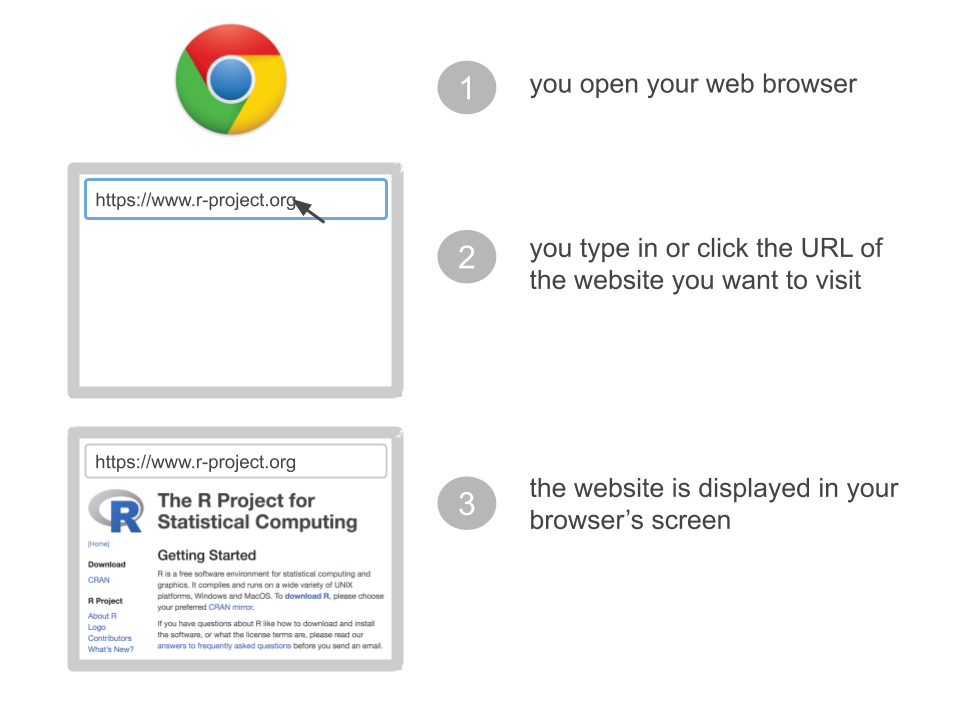
\includegraphics[width=0.7\linewidth]{images/http/web-scheme1} 

}

\caption{Surfing the web}\label{fig:unnamed-chunk-4}
\end{figure}

What exactly is happening ``behind the scenes''?

\begin{itemize}
\item
  People access websites using software called a \textbf{Web browser} (e.g.~Google
  Chrome, Safari, Firefox)
\item
  A browser is a software that, among other things, \textbf{requests} information
  (e.g.~request to access R project's website)
\item
  Using more proper language, the browser in your computer is the
  \textbf{client that requests} a variety of resources (e.g.~pages, images, videos,
  audio, scripts)
\item
  The client's request is sent to \textbf{Web servers}
\item
  A \textbf{server} is the software-computer in charge of \textbf{serving} the resources
  that the clients request.
\item
  The server \textbf{sends responses} back to the client
\end{itemize}

\begin{figure}

{\centering 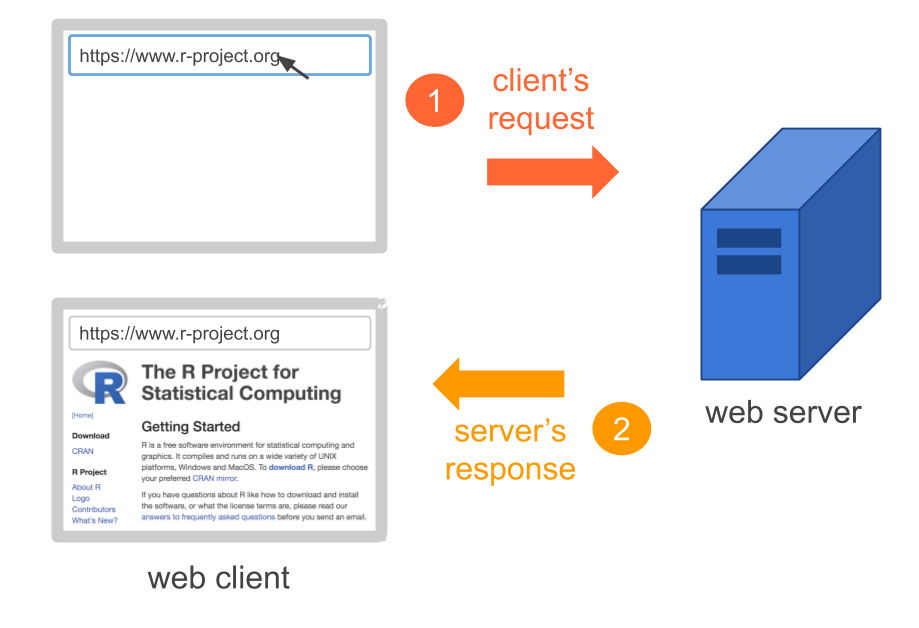
\includegraphics[width=0.7\linewidth]{images/http/web-scheme2} 

}

\caption{Client makes a request, and the serve responds}\label{fig:unnamed-chunk-5}
\end{figure}

To be more accurate, the server is the software that allows the computer
to communicate with other computers; however, it is common to use the term
``server'' to refer to the computer running the software, which also contains
other files and programs.
Simply put, a server is basically a computer connected to the Internet. The
Internet, in turn, is just a network of connected computers forming a system of
standards and rules. The purpose of connecting computers together is to share
information.

The job of the server software is to wait for a request for information, then
retrieve and send that information back to the client(s) as fast as possible.
In other words, Web servers have a full time job, waiting for requests from
Web browsers all over the world.

\hypertarget{how-does-the-web-work}{%
\section{How Does the Web Work?}\label{how-does-the-web-work}}

Now that we have the high level intuition of clients making requests, and
servers sending responses back to clients, let's describe things in more
detail.

To make web pages, programmers, developers and designers create files written
in a special type of syntax called \textbf{HyperText Markup Language} or HTML for
short. These files are stored in a Web server.

\begin{figure}

{\centering 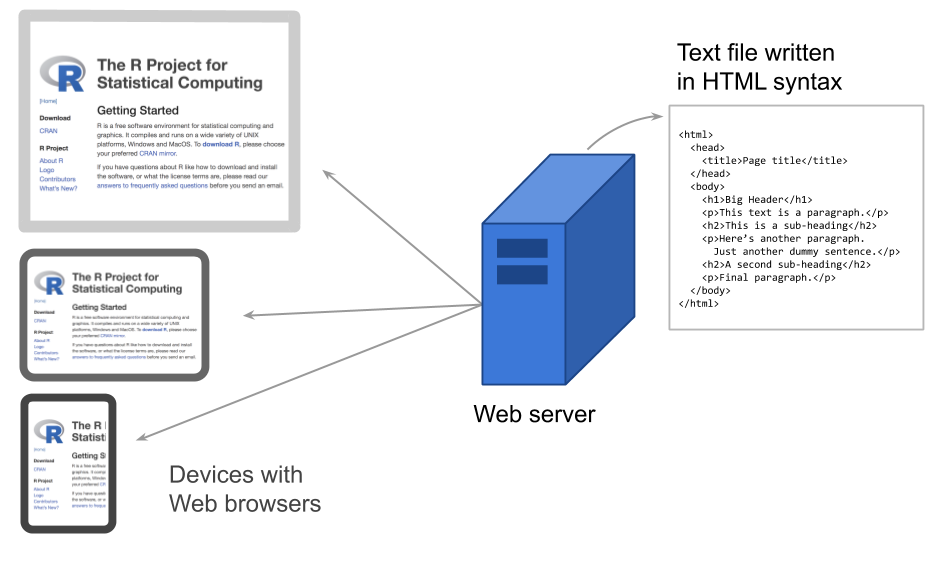
\includegraphics[width=0.8\linewidth]{images/http/web-scheme3} 

}

\caption{HTML files are the building blocks of web pages}\label{fig:unnamed-chunk-6}
\end{figure}

To be more precise, Web servers store more than one single HTML file. In
practice, websites are made of several directories containing various types of
files (image files, audio files, video files, scripts, etc).

\begin{figure}

{\centering 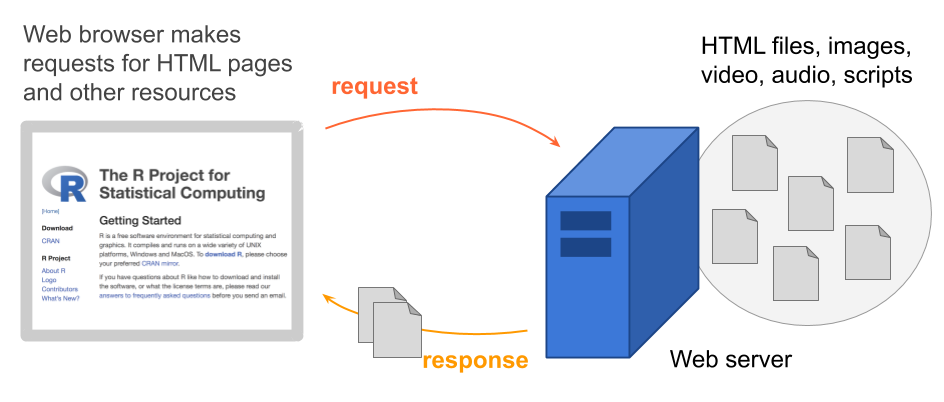
\includegraphics[width=0.8\linewidth]{images/http/web-scheme5} 

}

\caption{Web server containing several types of files, not just HTML files}\label{fig:unnamed-chunk-7}
\end{figure}

Once HTML files are put on the web server, any browser (e.g.~Chrome, Safari,
Firefox, Explorer) can retrieve the web page over the internet. The browser
on your laptop, on your tablet, on your cellphone, you name it. As long as the
device you are using is connected to the internet, the browser will retrieve
the web page. The HTML content in the web page tells the browser everything it
needs to know to display the page.

\begin{figure}

{\centering 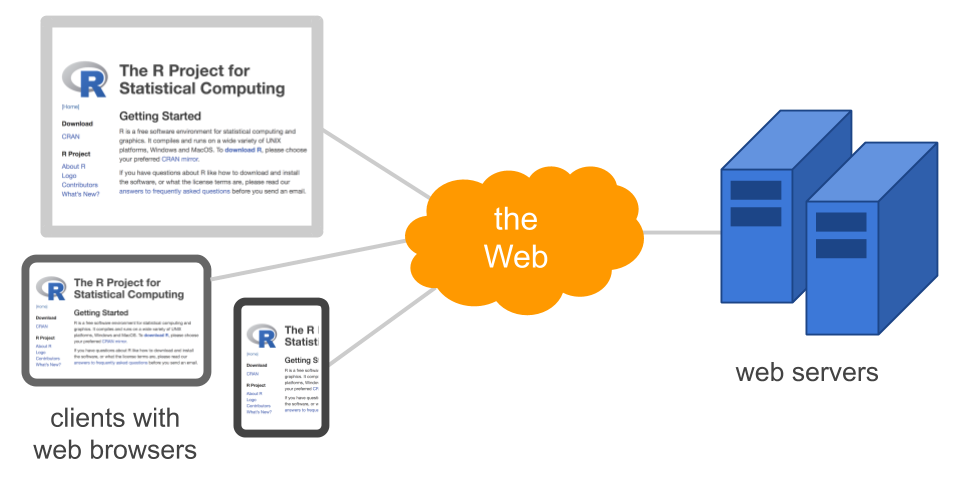
\includegraphics[width=0.75\linewidth]{images/http/web-scheme4} 

}

\caption{Diagram of the Web}\label{fig:unnamed-chunk-8}
\end{figure}

On a side note, it's important to distinguish the Internet from the Web. The
Web, originally called the World Wide Web, is just one option to share
information over the Internet. What characterizes the Web is that it allows
documents to be linked to one another using \emph{hypertext} links or hyperlinks,
thus forming a web of interconnected resources.

\hypertarget{in-summary}{%
\subsubsection*{In Summary}\label{in-summary}}
\addcontentsline{toc}{subsubsection}{In Summary}

\begin{itemize}
\item
  The Web is a massive distributed information system connecting software
  and computers to share information.
\item
  The software and computers that form the Web are divided into two types:
  \emph{clients} and \emph{servers}.
\item
  The way clients and servers dialogue between each other is by following
  formal \textbf{protocols of communication}.
\item
  The main type of protocol that clients and servers use is the HyperText
  Transfer Protocol (HTTP).
\item
  But there are other ways in which computers can exchange information such as
  email, file transfer (FTP), and many others.
\end{itemize}

\hypertarget{http}{%
\chapter{Basics of HTTP}\label{http}}

In the preceding chapter you were given a high-level description about how the
Web works. In this chapter we take the next step to give you a basic introduction
to HTTP which is the protocol that servers and browsers use to communicate and
exchange information on the Web.

\hypertarget{what-is-http}{%
\section{What is HTTP?}\label{what-is-http}}

HTTP is the acronym for \emph{Hypertext Transfer Protocol}. Perhaps the two most
important terms in this name are \emph{Protocol} and \emph{Transfer}.

According to the dictionary, a \textbf{protocol} is:

\begin{quote}
``A system of rules that explain the correct conduct and procedures to be
followed in formal situations''
\end{quote}

In turn, a \textbf{transfer protocol} is a communications protocol:

\begin{quote}
``A communications protocol is a system of digital rules for data exchange
within or between computers.''
\end{quote}

So, what is HTTP? Simply put, HTTP is the set of rules for transferring things
such as text, images, sound, video and other multimedia files over the Web.

\hypertarget{a-quick-introduction-to-http}{%
\section{A quick introduction to HTTP}\label{a-quick-introduction-to-http}}

\begin{itemize}
\item
  Whenever you surf the web, your browser sends \textbf{HTTP request messages}
\item
  the HTTP requests are sent to Web servers
\item
  web servers handle these requests by returning \textbf{HTTP response messages}
\item
  the messages contain the requested resource(s)
\end{itemize}

\hypertarget{http-example}{%
\subsection{HTTP Example}\label{http-example}}

Suppose we open the browser in order to visit R project's homepage

\begin{verbatim}
https://www.r-project.org
\end{verbatim}

Although we don't see it, there's is a client-server dialogue taking place,
illustrated in the diagram below:

\begin{figure}

{\centering 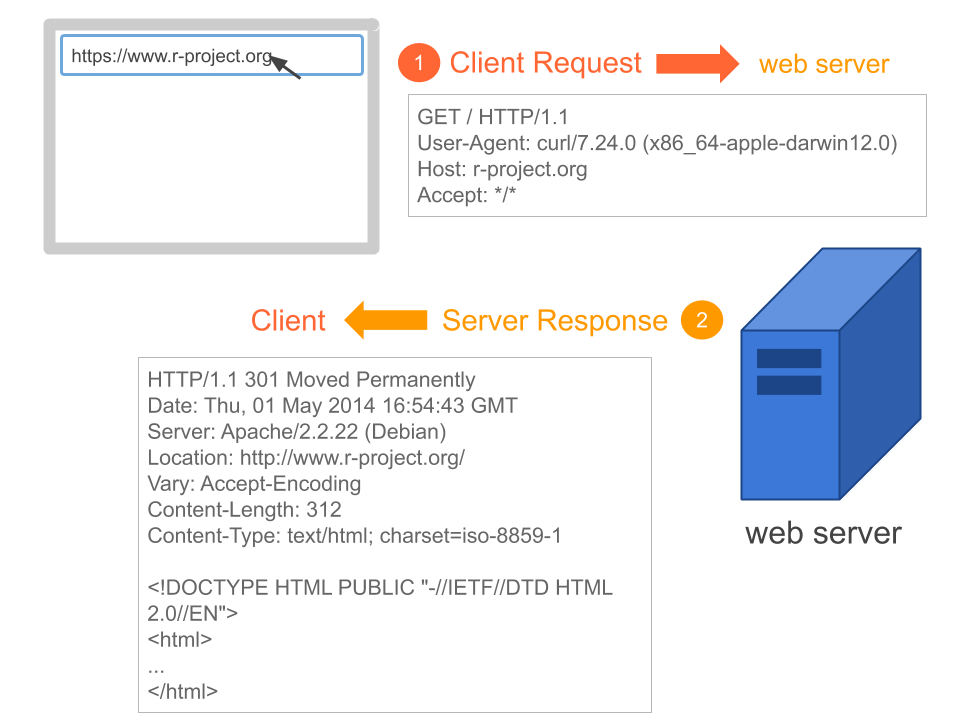
\includegraphics[width=0.7\linewidth]{images/http/web-scheme6} 

}

\caption{Client makes a request, and the serve responds}\label{fig:unnamed-chunk-10}
\end{figure}

Using Chrome's \textbf{DevTools} (developer tools), we can see the associated
information related to the HTTP ``conversation'' between the client and the
server. We provide the content of this dialogue in the following block:

\begin{figure}

{\centering 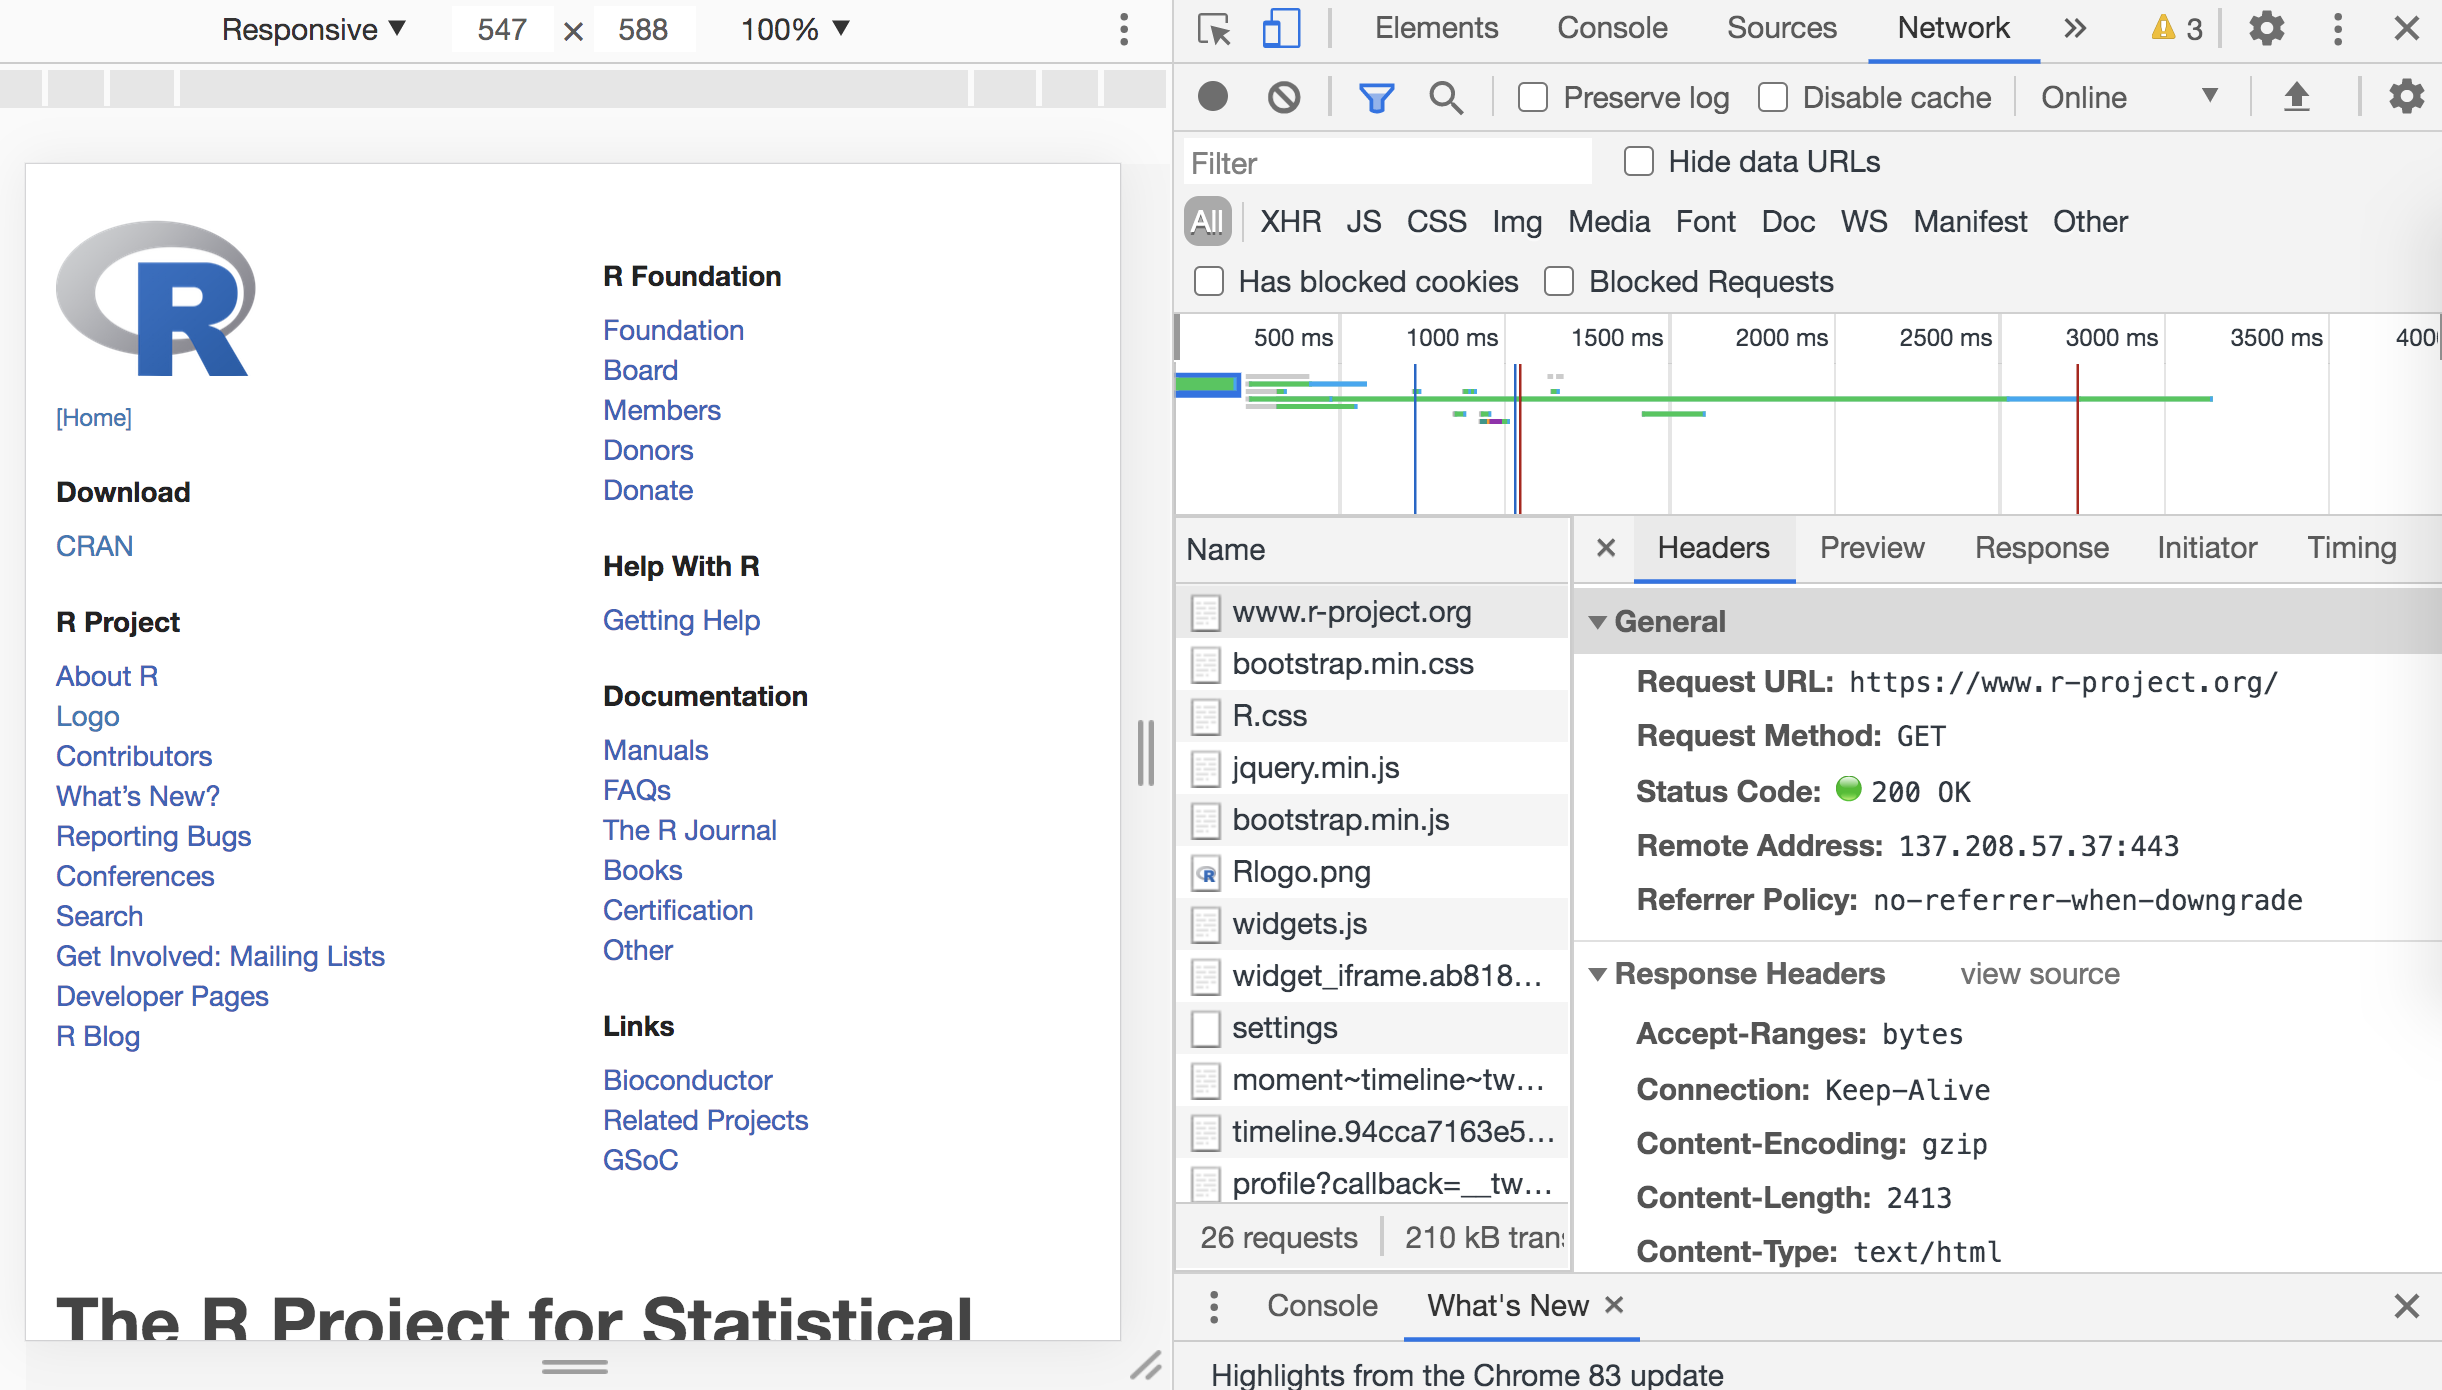
\includegraphics[width=0.9\linewidth]{images/http/web-http-devtools} 

}

\caption{Inspecting HTTP messages via DevTools}\label{fig:unnamed-chunk-11}
\end{figure}

Think of an HTTP request as a set of information sent to the server. When the
server receives the request, it (the server) processes the information and
provides a response back to the client.

When you visit a URL in your web browser, say R's project website
(\texttt{https://www.r-project.org}), an HTTP request is made and the response is
rendered by the browser as the website you see. Although we don't see the
``dialogue'' between client and server, it is possible to inspect this
interaction using the development tools in a browser such as Chrome's DevTools
(like the screenshot above).

\begin{figure}

{\centering 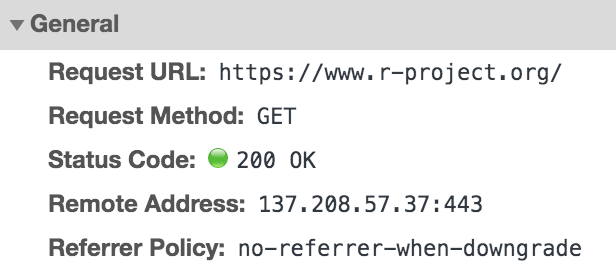
\includegraphics[width=0.4\linewidth]{images/http/web-http-headers} 

}

\caption{DevTools menu tab for inspecting HTTP messages}\label{fig:unnamed-chunk-12}
\end{figure}

The above is a screen-capture in which we can see that the request is composed
of a URL (R's project website), and a request method (\texttt{GET}) which is what the
browser employs to access a website.

\hypertarget{http-request}{%
\subsection{HTTP Request}\label{http-request}}

There are several components of an HTTP request (see figure below), but we
will focus on the most relevant:

\begin{itemize}
\item
  \texttt{URL}: the address or endpoint for the request
\item
  HTTP method or verb: a specific method invoked on the endpoint
  (\texttt{GET}, \texttt{POST}, \texttt{DELETE}, \texttt{PUT})
\item
  Headers: additional data sent to the server, such as who is making the request
  and what type of response is expected
\item
  Body: data sent to the server outside of the headers, common for \texttt{POST} and
  \texttt{PUT} requests
\end{itemize}

\begin{figure}

{\centering 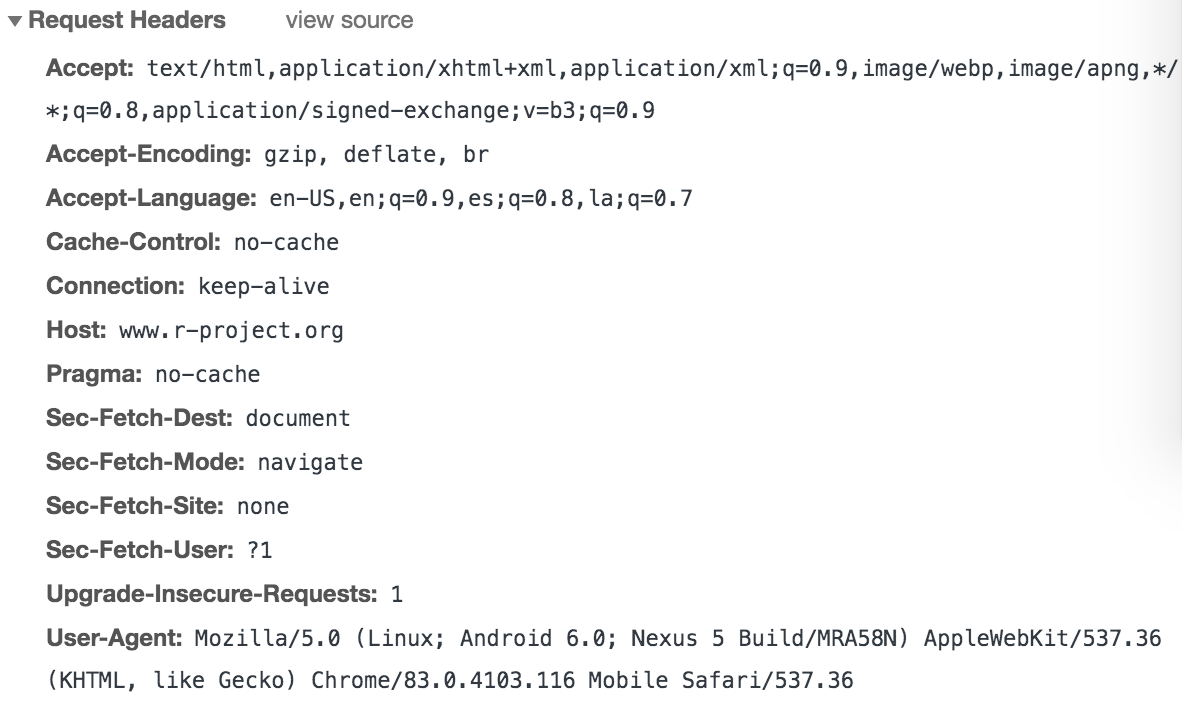
\includegraphics[width=0.9\linewidth]{images/http/web-http-request-headers} 

}

\caption{HTTP request headers}\label{fig:unnamed-chunk-13}
\end{figure}

\hypertarget{http-response}{%
\subsection{HTTP Response}\label{http-response}}

The response headers include the HTTP status code that informs the client how
the request was received. There are also other details about the
content delivered by the server. In the above example accessing
www.r-project.com, we can see the status code success \texttt{200}, along with other
details about the response content. Notice that the returned content is HTML.
This HTML content is what the browser renders into a webpage.

\begin{figure}

{\centering 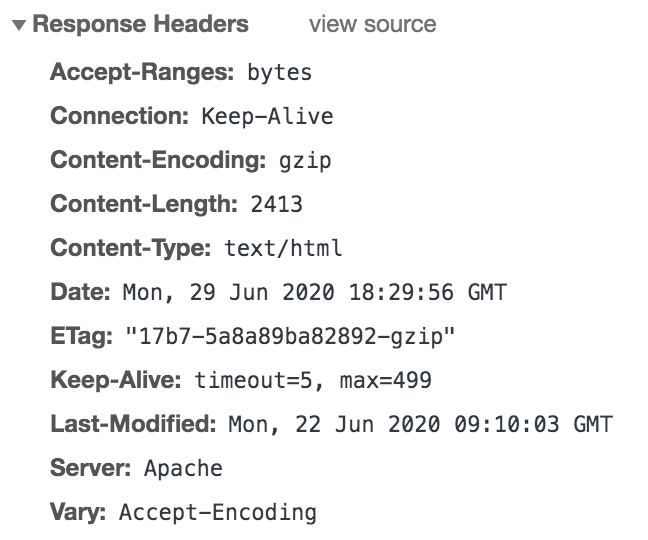
\includegraphics[width=0.5\linewidth]{images/http/web-http-response-headers} 

}

\caption{HTTP response headers}\label{fig:unnamed-chunk-14}
\end{figure}

\hypertarget{anatomy-of-an-http-message}{%
\section{Anatomy of an HTTP message}\label{anatomy-of-an-http-message}}

HTTP messages consist of 2 parts (separated by a blank line)

\begin{enumerate}
\def\labelenumi{\arabic{enumi})}
\tightlist
\item
  A message \textbf{header}

  \begin{itemize}
  \tightlist
  \item
    the first line in the header is the request/response line
  \item
    the rest of the lines are \emph{headers} formed of \texttt{name:value} pairs
  \end{itemize}
\item
  An optional message \textbf{body}
\end{enumerate}

The client (your browser) sends a request to the server:

\begin{verbatim}
GET / HTTP/1.1
User-Agent: curl/7.24.0 (x86_64-apple-darwin12.0) libcurl/7.24.0 OpenSSL/0.9.8y zlib/1.2.5
Host: r-project.org
Accept: */*
\end{verbatim}

\begin{itemize}
\tightlist
\item
  The first line is the \textbf{request line} which contains: \texttt{GET\ /\ HTTP/1.1}
\item
  The rest of the \emph{headers} are just \texttt{name:value} pairs,
  e.g.~\texttt{Host:\ r-project.org}
\end{itemize}

The server sends a \textbf{response} to the client:

\begin{verbatim}
HTTP/1.1 301 Moved Permanently
Date: Thu, 01 May 2014 16:54:43 GMT
Server: Apache/2.2.22 (Debian)
Location: http://www.r-project.org/
Vary: Accept-Encoding
Content-Length: 312
Content-Type: text/html; charset=iso-8859-1
 
<!DOCTYPE HTML PUBLIC "-//IETF//DTD HTML 2.0//EN">
<html>
...
</html>
\end{verbatim}

\begin{itemize}
\tightlist
\item
  The first line is the \textbf{status line} which contains: \texttt{GET\ /\ HTTP/1.1}
\item
  The next lines contain \textbf{header values}
\item
  The \textbf{body} message appears after the blank line, in this case is the
  content of the HTML page
\end{itemize}

\hypertarget{http-methods}{%
\subsection{HTTP Methods}\label{http-methods}}

Here's a table with HTTP methods, and their descriptions

\begin{longtable}[]{@{}
  >{\raggedright\arraybackslash}p{(\columnwidth - 2\tabcolsep) * \real{0.4583}}
  >{\raggedright\arraybackslash}p{(\columnwidth - 2\tabcolsep) * \real{0.5417}}@{}}
\toprule\noalign{}
\begin{minipage}[b]{\linewidth}\raggedright
Method
\end{minipage} & \begin{minipage}[b]{\linewidth}\raggedright
Description
\end{minipage} \\
\midrule\noalign{}
\endhead
\bottomrule\noalign{}
\endlastfoot
\texttt{GET} & retrieves whatever information is identified by the Request-URI \\
\texttt{POST} & request with data enclosed in the request body \\
\texttt{HEAD} & identical to GET except that the server MUST NOT return a message-body in the response \\
\texttt{PUT} & requests that the enclosed entity be stored under the supplied Request-URI \\
\texttt{DELETE} & requests that the origin server delete the resource identified by the Request-URI \\
\texttt{TRACE} & invokes a remote, application-layer loop-back of the request message \\
\texttt{CONNECT} & for use with a proxy that can dynamically switch to being a tunnel \\
\end{longtable}

So far we've seen that:

\begin{itemize}
\item
  The HTTP protocol is a standardized method for transferring data or documents
  over the Web
\item
  The clients' requests and the servers' responses are handled via the HTTP
  protocol
\item
  There are 2 types of HTTP messages: \textbf{requests} and \textbf{responses}
\item
  We don't actually see HTTP messages but they are there behind the scenes
\end{itemize}

\hypertarget{part-xml}{%
\part{XML}\label{part-xml}}

\hypertarget{xml}{%
\chapter{Basics of XML}\label{xml}}

The goal of this chapter is to give you a crash introduction to XML so that
you can get a good grasp of this format for the rest of the book.

\begin{itemize}
\item
  Large amounts of data and information are stored, shared and distributed
  using XML-dialects.
\item
  They are widely adopted and used in many applications.
\item
  Working with data from the Web often means dealing with some kind of XML
  dialect.
\end{itemize}

\hypertarget{what-is-xml}{%
\section{What is XML?}\label{what-is-xml}}

XML stands for \emph{eXtensible Markup Language}

Let's dissect the meaning of this acronym. On one hand, XML is a markup language.
which means, XML defines a set of rules for encoding information in a format
that is both human-readable and machine-readable.

Compared to other types of markup languages (e.g LaTeX, Markdown), XML is used
to describe data. To be more precise, XML is a standard for the semantic,
\textbf{hierarchical} representation of data. This is an important aspect of XML
and any of its dialects, because data is represented following a hierarchy.

For instance, one way to organize data is in a table. Conceptually, all elements
are stored in cells of a grid structure of rows and columns. Another way to
organize data is with hierarchies, that can be visually represented with tree
like structures. This latter form of organizing data is what XML uses.

The second aspect, ``extensible'', means that we can define any number of new
formats to represent any kind of data. Therefore, it is extensible.
This is a very interesting aspect of XML because it provides a flexible
framework to create new formats for describing and representing data.

\hypertarget{comments}{%
\subsubsection*{Comments}\label{comments}}
\addcontentsline{toc}{subsubsection}{Comments}

Before moving on, we want to clarify some key terms.

A \textbf{markup} is a sequence of characters or other symbols inserted at certain
places in a document to indicate either:

\begin{itemize}
\tightlist
\item
  how the content should be displayed when printed or in screen
\item
  describe the document's structure
\end{itemize}

A Markup Language is a system for annotating (i.e.~marking) a document in a
way that the content is distinguished from its representation (e.g.~LaTeX,
PostScript, HTML, SVG)

\hypertarget{marks-in-xml}{%
\subsection{Marks in XML}\label{marks-in-xml}}

In XML (as well as in HTML) the marks (also known as tags) are defined using
angle brackets: \texttt{\textless{}\ \textgreater{}}.

For example:

\begin{verbatim}
<mark>Text marked with special tag</mark>
\end{verbatim}

The concept of extensibility means that we can define our own marks, the order
in which they occur, and how they should be processed. For example we could
define marks such as:

\begin{itemize}
\tightlist
\item
  \texttt{\textless{}my\_mark\textgreater{}}
\item
  \texttt{\textless{}awesome\textgreater{}}
\item
  \texttt{\textless{}boring\textgreater{}}
\item
  \texttt{\textless{}pathetic\textgreater{}}
\end{itemize}

Before moving on, we should mention that XML is NOT:

\begin{itemize}
\tightlist
\item
  a programming language
\item
  a network transfer protocol
\item
  a database
\end{itemize}

Instead, XML is:

\begin{itemize}
\tightlist
\item
  more than a markup language
\item
  a generic language that provides structure and syntax for representing any
  type of information
\item
  a meta-language: it allows us to create or define other languages
\end{itemize}

Here are some famous examples of XML dialects:

\begin{itemize}
\item
  \textbf{KML} (Keyhole Markup Language) for describing geo-spatial information used
  in Google Earth, Google Maps, Google Sky
\item
  \textbf{SVG} (Scalable Vector Graphics) for visual graphical displays of
  two-dimensional graphics with support for interactivity and animation
\item
  \textbf{PMML} (Predictive Model Markup Language) for describing and exchanging
  models produced by data mining and machine learning algorithms
\item
  \textbf{RSS} (Rich Site Summary) feeds for publishing blog entries
\item
  \textbf{SDMX} (Statistical Data and Metadata Exchange) for organizing and
  exchanging statistical information
\item
  \textbf{SBML} (Systems Biology Markup Language) for describing biological systems
\end{itemize}

\hypertarget{minimalist-example}{%
\subsection{Minimalist Example}\label{minimalist-example}}

Let's consider a handful of XML examples using one of my favorite movies:
\emph{Good Will Hunting}, a 1997 American psychological drama film directed by Gus
Van Sant, and written by Ben Affleck and Matt Damon.

\begin{figure}

{\centering 
\includegraphics[width=0.5\linewidth]{images/xml/xml-good-will-hunting} 

}

\caption{Good Will Hunting (Directed by Gus Van Sant, 1997)}\label{fig:unnamed-chunk-16}
\end{figure}

\hypertarget{ultra-simple-example}{%
\subsubsection*{Ultra Simple example}\label{ultra-simple-example}}
\addcontentsline{toc}{subsubsection}{Ultra Simple example}

Let's see an ultra simple XML example:

\begin{verbatim}
<movie>
  Good Will Hunting
</movie>
\end{verbatim}

\begin{itemize}
\tightlist
\item
  one single element \emph{movie}
\item
  start-tag: \texttt{\textless{}movie\textgreater{}}
\item
  end-tag: \texttt{\textless{}/movie\textgreater{}}
\item
  content: \texttt{Good\ Will\ Hunting}
\end{itemize}

\hypertarget{elements-with-attributes}{%
\subsubsection*{Elements with attributes}\label{elements-with-attributes}}
\addcontentsline{toc}{subsubsection}{Elements with attributes}

XML elements can have attributes, for example:

\begin{verbatim}
<movie mins="126" lang="en">
  Good Will Hunting
</movie>
\end{verbatim}

\begin{itemize}
\tightlist
\item
  attributes: \texttt{mins} (minutes) and \texttt{lang} (language)
\item
  attributes are attached to the element's start tag
\item
  attribute values must be quoted!
\end{itemize}

\hypertarget{elements-within-other-elements}{%
\subsubsection*{Elements within other elements}\label{elements-within-other-elements}}
\addcontentsline{toc}{subsubsection}{Elements within other elements}

XML elements may contain other elements, for example:

\begin{verbatim}
<movie mins="126" lang="en">
  <title>Good Will Hunting</title>
  <director>Gus Van Sant</director>
  <year>1998</year>
  <genre>drama</genre>
</movie>
\end{verbatim}

\begin{itemize}
\item
  an xml element may contain other elements
\item
  \emph{movie} contains several elements: \emph{title}, \emph{director}, \emph{year}, \emph{genre}
\end{itemize}

\hypertarget{more-embedded-elements}{%
\subsubsection*{More Embedded elements}\label{more-embedded-elements}}
\addcontentsline{toc}{subsubsection}{More Embedded elements}

As you can tell, the xml element \emph{movie} has a now a hierarchy. We can make it
more interesting by including more elements inside \emph{director}.

\begin{verbatim}
<movie mins="126" lang="en">
  <title>Good Will Hunting</title>
  <director>
    <first_name>Gus</first_name>
    <last_name>Van Sant</last_name>
  </director>
  <year>1998</year>
  <genre>drama</genre>
</movie>
\end{verbatim}

Formally, we say that \emph{director} has two child elements: \texttt{first\_name} and
\texttt{last\_name}.

\hypertarget{tree-structure-in-xml}{%
\subsubsection*{Tree Structure in XML}\label{tree-structure-in-xml}}
\addcontentsline{toc}{subsubsection}{Tree Structure in XML}

We can graphically display the structure of an XML document with a tree
diagram, like the following one:

\begin{figure}

{\centering 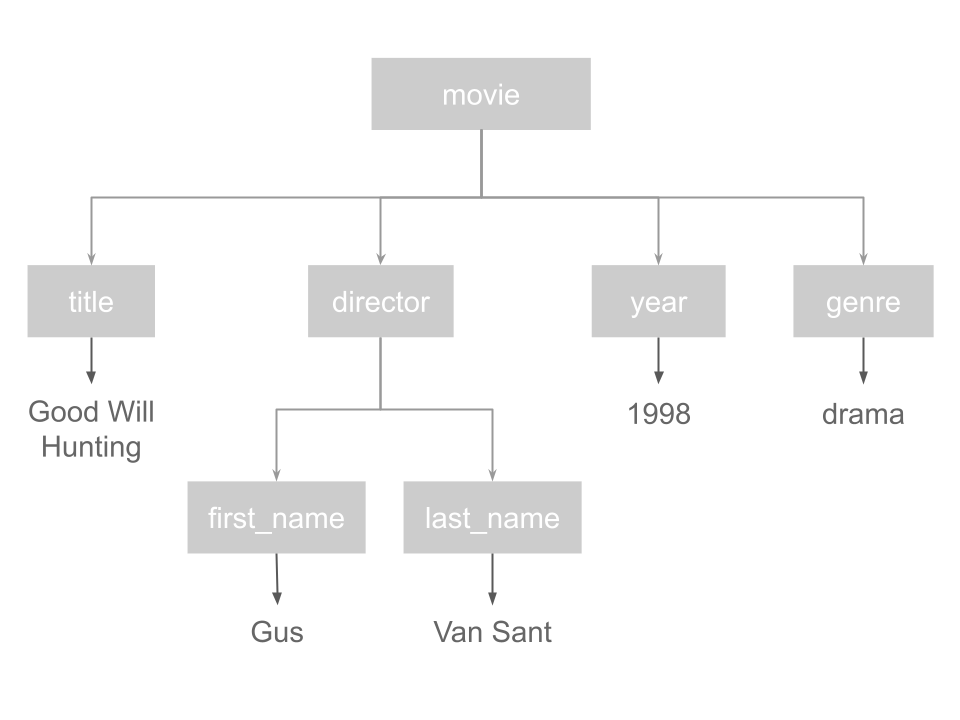
\includegraphics[width=0.65\linewidth]{images/xml/xml-tree1} 

}

\caption{XML tree structure}\label{fig:unnamed-chunk-17}
\end{figure}

\begin{itemize}
\item
  An XML document can be represented with a \textbf{tree structure}
\item
  An XML document must have \textbf{one single Root} element
\item
  The \texttt{Root} may contain \texttt{child} elements
\item
  A \texttt{child} element may contain \texttt{subchild} elements
\end{itemize}

\hypertarget{well-formedness}{%
\subsection{Well Formedness}\label{well-formedness}}

We say that an XML document is \textbf{well-formed} when it obeys the basic syntax
rules of XML. Some of those rules are:

\begin{itemize}
\tightlist
\item
  one root element containing the rest of elements
\item
  properly nested elements
\item
  self-closing tags
\item
  attributes appear in start-tags of elements
\item
  attribute values must be quoted
\item
  element names and attribute names are case sensitive
\end{itemize}

Does it matter if an XML document is not Well-formed? Not well-formed XML
documents produce potentially fatal errors or warnings when parsed.

Keep in mind that documents may be well-formed but not valid. Well-formed just
guarantees that the document meets the basic XML structure, not that the content
is valid.

\hypertarget{additional-xml-elements}{%
\subsection{Additional XML Elements}\label{additional-xml-elements}}

Some Additional Elements

\begin{verbatim}
<?xml version="1.0"? encoding="UTF-8" ?>
<![CDATA[ a > 5 & b < 10 ]]>
<?GS print(format = TRUE)>
<!DOCTYPE Movie>
<!-- This is a commet -->
<movie mins="126" lang="en">
  <title>Good Will Hunting</title>
  <director>
    <first_name>Gus</first_name>
    <last_name>Van Sant</last_name>
  </director>
  <year>1998</year>
  <genre>drama</genre>
</movie>
\end{verbatim}

The following table lists some of the common additional XML elements:

\begin{longtable}[]{@{}
  >{\raggedright\arraybackslash}p{(\columnwidth - 4\tabcolsep) * \real{0.2656}}
  >{\raggedright\arraybackslash}p{(\columnwidth - 4\tabcolsep) * \real{0.4219}}
  >{\raggedright\arraybackslash}p{(\columnwidth - 4\tabcolsep) * \real{0.3125}}@{}}
\toprule\noalign{}
\begin{minipage}[b]{\linewidth}\raggedright
Markup
\end{minipage} & \begin{minipage}[b]{\linewidth}\raggedright
Name
\end{minipage} & \begin{minipage}[b]{\linewidth}\raggedright
Description
\end{minipage} \\
\midrule\noalign{}
\endhead
\bottomrule\noalign{}
\endlastfoot
\texttt{\textless{}?xml\ \textgreater{}} & XML Declaration & Identifies content as an XML document \\
\texttt{\textless{}?PI\ \textgreater{}} & Processing Instruction & Processing instructions passed to application PI \\
\texttt{\textless{}!DOCTYPE\ \textgreater{}} & Document-type Declaration & Defines the structure of an XML document \\
\texttt{\textless{}!{[}CDATA{[}\ {]}{]}\textgreater{}} & CDATA Character Data & Anything inside a CDATA is ignored by the parser \\
\texttt{\textless{}!-\/-\ \ -\/-\textgreater{}} & Comment & For writing comments \\
\end{longtable}

\hypertarget{another-example}{%
\subsection{Another Example}\label{another-example}}

Let's go back to the \emph{movie} example, but now let's see how the content of
our hypothetical XML document should look like:

\begin{verbatim}
<?xml version="1.0"?>
<!DOCTYPE movies>
<movie mins="126" lang="en">
  <!-- this is a comment -->
  <title>Good Will Hunting</title>
  <director>
    <first_name>Gus</first_name>
    <last_name>Van Sant</last_name>
  </director>
  <year>1998</year>
  <genre>drama</genre>
</movie>
\end{verbatim}

Each Node can have

\begin{itemize}
\tightlist
\item
  a Name
\item
  any number of attributes
\item
  optional content
\item
  other nested elements
\end{itemize}

\hypertarget{wrapping-up}{%
\subsection{Wrapping-Up}\label{wrapping-up}}

About XML

\begin{itemize}
\tightlist
\item
  designed to store and transfer data
\item
  designed to be self-descriptive
\item
  tags are not predefined and can be extended
\item
  a generic language that provides structure and syntax for many markup dialects
\item
  is a syntax or format for defining markup languages
\item
  a standard for the semantic, hierarchical representation of data
\item
  provides a general approach for representing all types of information dialects
\end{itemize}

\hypertarget{parsing-xml}{%
\chapter{Parsing XML}\label{parsing-xml}}

The goal of this chapter is to describe how we can parse XML content
with the R package \texttt{xml2}

You will need the following packages

\begin{Shaded}
\begin{Highlighting}[]
\FunctionTok{library}\NormalTok{(xml2)}
\FunctionTok{library}\NormalTok{(stringr)}
\end{Highlighting}
\end{Shaded}

We'll cover a variety of situations you most likely will find yourself dealing
with:

\begin{itemize}
\item
  R package \texttt{"xml2"}
\item
  Navigating the XML tree structure
\item
  XPath expressions
\end{itemize}

\hypertarget{what-is-parsing}{%
\section{What is parsing?}\label{what-is-parsing}}

Getting data from the web often involves reading and processing content from
XML and HTML documents. This is known as \textbf{parsing}.

The dictionary defines ``parse'' as:

\begin{quote}
analyze (a sentence) into its parts and describe their syntactic roles.
\end{quote}

In regards to ``computing'', parse has to do with:

\begin{quote}
analyze (a string or text) into logical syntactic components, typically in
order to test conformability to a logical grammar.

an act of or the result obtained by parsing a string or a text.
\end{quote}

According to Wikipedia, a parser is:

\begin{quote}
A parser is a software component that takes input data (frequently text) and
builds a data structure ---often some kind of parse tree, abstract syntax
tree or other hierarchical structure--- giving a structural representation of
the input, checking for correct syntax in the process
\end{quote}

\hypertarget{r-package-xml2}{%
\section{\texorpdfstring{R package \texttt{"xml2"}}{R package "xml2"}}\label{r-package-xml2}}

The package \texttt{"xml2"} is designed for one major purpose, namely, to parse
XML and HTML content. Remember that HTML is one the countless XML dialects.

As of this writing, \texttt{"xml2"} has minimal functionality for writing
content in XML. Hadley Wickham has mentioned that he plans to add more functions
for writing XML. So it is possible that in the future, \texttt{"xml2"} integrates
more writing-XML functionality. Having said that, we will focus exclusively on
reading XML content.

We'll cover 4 major types of tasks that we can perform with \texttt{"xml2"}

\begin{itemize}
\tightlist
\item
  parsing (ie \emph{reading}) xml / html content
\item
  obtaining descriptive information about parsed contents
\item
  navigating the tree structure (i.e.~accessing its components)
\item
  querying and extracting data from parsed contents
\end{itemize}

\hypertarget{parsing-functions}{%
\subsection{Parsing Functions}\label{parsing-functions}}

There are two main parsing functions:

\begin{itemize}
\item
  \texttt{read\_xml()}
\item
  \texttt{read\_html()}
\end{itemize}

For XML files in general, you should use \texttt{read\_xml()}. For HTML files, then
it's better to use \texttt{read\_html()} because it is more robust, and can handle
no well-formed HTML files, which are not uncommon to deal with in practice.

The main input for these reading functions is either a string, an R connection,
or a raw vector.

The string can be either a path, a URL or literal xml. URL's will be converted
into connections either using \texttt{base::url()} or, if installed, \texttt{curl::curl()}.
Local paths ending in .gz, .bz2, .xz, .zip will be automatically uncompressed.

Both \texttt{read\_xml()} and \texttt{read\_html()} return an object of class \texttt{"xml\_document"}.

Let's see an example. Consider one of the examples from the previous chapter,
for instance some content in XML:

\begin{verbatim}
<movie mins="126" lang="en">
  <title>Good Will Hunting</title>
  <director>
    <first_name>Gus</first_name>
    <last_name>Van Sant</last_name>
  </director>
  <year>1998</year>
  <genre>drama</genre>
</movie>
\end{verbatim}

For illustration purposes, let's take the XML content, treating it as a single
character string, that we then pass to \texttt{read\_xml()}:

\begin{Shaded}
\begin{Highlighting}[]
\CommentTok{\# toy example with xml string}
\NormalTok{movie }\OtherTok{\textless{}{-}} \FunctionTok{read\_xml}\NormalTok{(}
\StringTok{"\textless{}movie\textgreater{}}
\StringTok{\textless{}title\textgreater{}Good Will Hunting\textless{}/title\textgreater{}}
\StringTok{\textless{}director\textgreater{}}
\StringTok{\textless{}first\_name\textgreater{}Gus\textless{}/first\_name\textgreater{}}
\StringTok{\textless{}last\_name\textgreater{}Van Sant\textless{}/last\_name\textgreater{}}
\StringTok{\textless{}/director\textgreater{}}
\StringTok{\textless{}year\textgreater{}1998\textless{}/year\textgreater{}}
\StringTok{\textless{}genre\textgreater{}drama\textless{}/genre\textgreater{}}
\StringTok{\textless{}/movie\textgreater{}"}\NormalTok{)}

\NormalTok{movie}
\CommentTok{\#\textgreater{} \{xml\_document\}}
\CommentTok{\#\textgreater{} \textless{}movie\textgreater{}}
\CommentTok{\#\textgreater{} [1] \textless{}title\textgreater{}Good Will Hunting\textless{}/title\textgreater{}}
\CommentTok{\#\textgreater{} [2] \textless{}director\textgreater{}\textbackslash{}n  \textless{}first\_name\textgreater{}Gus\textless{}/first\_name\textgreater{}\textbackslash{}n  \textless{}last\_name\textgreater{}Van Sant\textless{}/last\_n ...}
\CommentTok{\#\textgreater{} [3] \textless{}year\textgreater{}1998\textless{}/year\textgreater{}}
\CommentTok{\#\textgreater{} [4] \textless{}genre\textgreater{}drama\textless{}/genre\textgreater{}}
\end{Highlighting}
\end{Shaded}

As we mention, the \texttt{movie} is an XML object:

\begin{Shaded}
\begin{Highlighting}[]
\FunctionTok{class}\NormalTok{(movie)}
\CommentTok{\#\textgreater{} [1] "xml\_document" "xml\_node"}
\end{Highlighting}
\end{Shaded}

This type of object has an internal structure in order to maintain the
hierarchical tree-structure of any XML content.

\hypertarget{working-with-parsed-documents}{%
\section{Working with parsed documents}\label{working-with-parsed-documents}}

Having parsed an XML / HTML document, we can use 2 main functions to start
working on the tree structure:

\begin{itemize}
\item
  \texttt{xml\_root()} gets access to the root node and its elements
\item
  \texttt{xml\_children()} gets access to the children nodes of a given node
\end{itemize}

\hypertarget{example-with-a-basic-xml-document}{%
\subsection{Example with a basic XML document}\label{example-with-a-basic-xml-document}}

Here's some content: a movie elements in XML syntax

\begin{figure}

{\centering 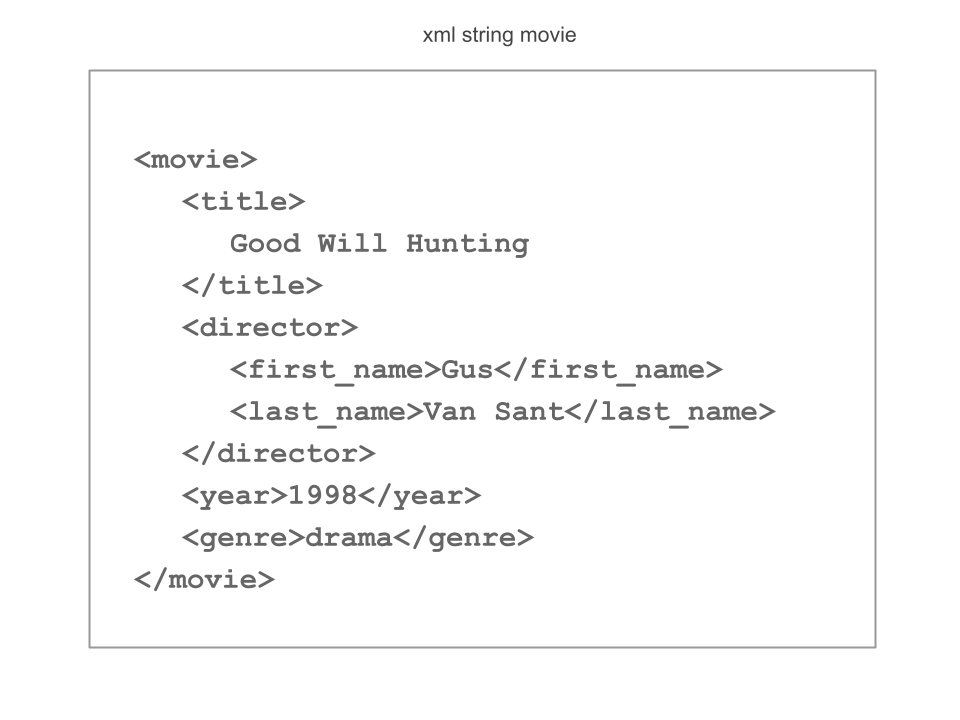
\includegraphics[width=0.7\linewidth]{images/xml/xml-movie1} 

}

\caption{XML Movie}\label{fig:unnamed-chunk-22}
\end{figure}

The following figure identifies the main nodes:

\begin{figure}

{\centering 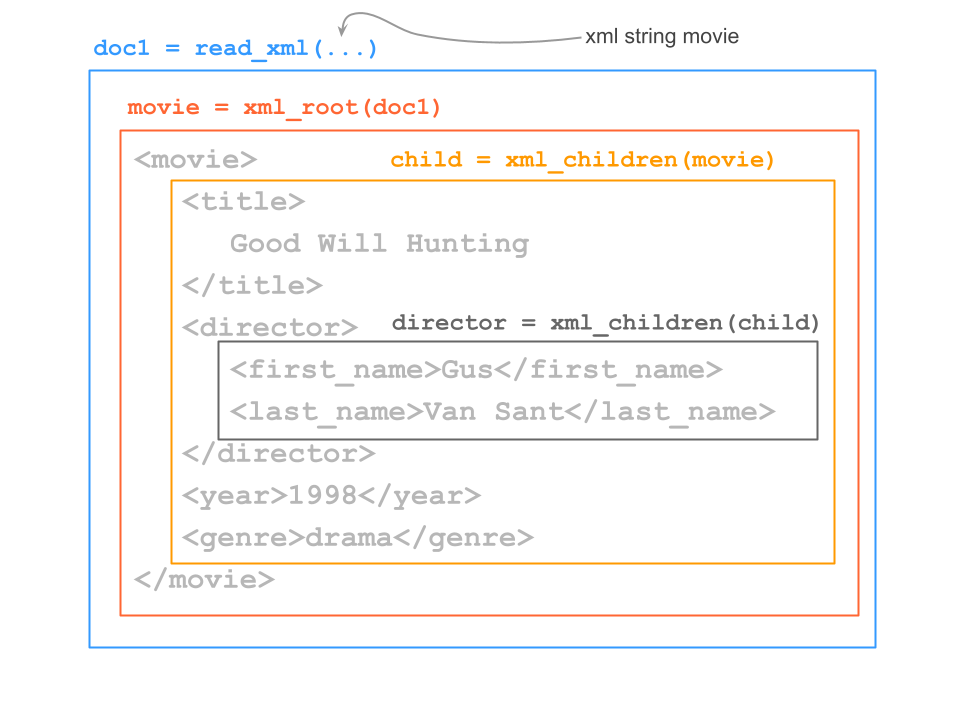
\includegraphics[width=0.7\linewidth]{images/xml/xml-movie2} 

}

\caption{XML Movie nodes}\label{fig:unnamed-chunk-23}
\end{figure}

Below is an abstract representation of an XML file, and its main nodes

\begin{figure}

{\centering 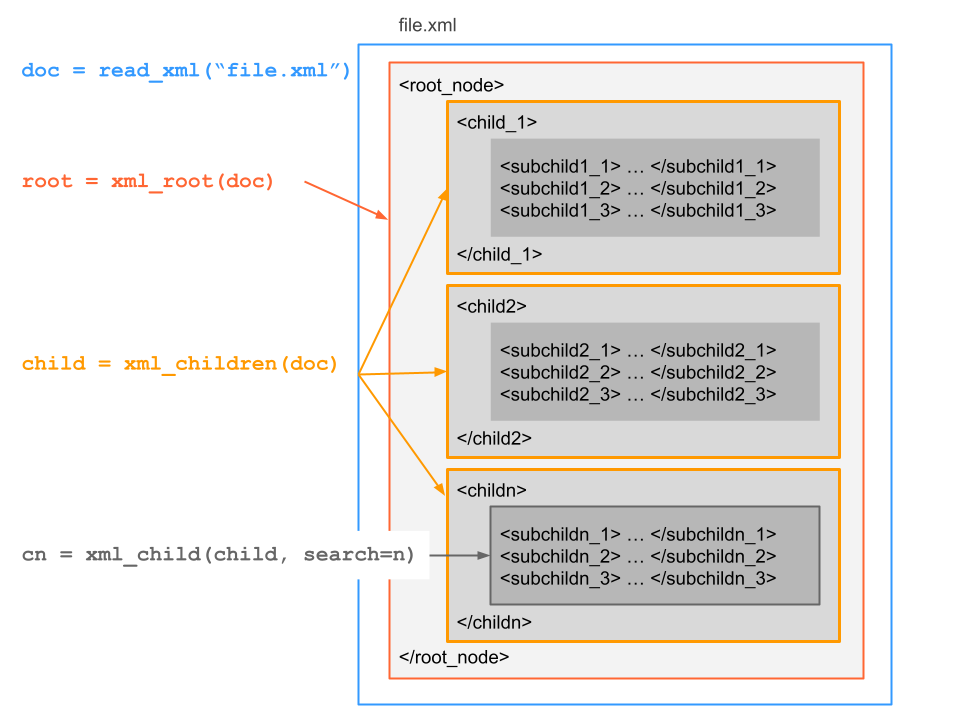
\includegraphics[width=0.85\linewidth]{images/xml/xml-functions} 

}

\caption{Functions of `xml2`}\label{fig:unnamed-chunk-24}
\end{figure}

\hypertarget{more-functions-in-xml2}{%
\subsection{\texorpdfstring{More Functions in \texttt{"xml2"}}{More Functions in "xml2"}}\label{more-functions-in-xml2}}

In addition to \texttt{xml\_root()} and \texttt{xml\_children()}, there are other functions
to parse the various kinds of content within a given node.

Here's a table with the main navigation functions. Keep in mind that the
applicability of the functions depends on the class of objects we are working on.

\begin{longtable}[]{@{}ll@{}}
\toprule\noalign{}
Function & Description \\
\midrule\noalign{}
\endhead
\bottomrule\noalign{}
\endlastfoot
\texttt{xml\_root()} & Returns root node \\
\texttt{xml\_children()} & Returns children nodes \\
\texttt{xml\_child()} & Returns specified children number \\
\texttt{xml\_name()} & Returns name of a node \\
\texttt{xml\_contents()} & Returns contents of a node \\
\texttt{xml\_text()} & Returns text \\
\texttt{xml\_length()} & Returns number of children nodes \\
\texttt{xml\_parents()} & Returns set of parent nodes \\
\texttt{xml\_siblings()} & Returns set of sibling nodes \\
\end{longtable}

\hypertarget{navigation-of-xml-html-tree}{%
\subsection{Navigation of XML / HTML Tree}\label{navigation-of-xml-html-tree}}

Let's consider the following XML content:

\begin{verbatim}
<movies>
     <movie mins="126" lang="eng">
        <title>Good Will Hunting</title>
        <director>
           <first_name>Gus</first_name>
           <last_name>Van Sant</last_name>
        </director>
        <year>1998</year>
        <genre>drama</genre>
     </movie>
     <movie mins="106" lang="spa">
        <title>Y tu mama tambien</title>
        <director>
           <first_name>Alfonso</first_name>
           <last_name>Cuaron</last_name>
        </director>
        <year>2001</year>
        <genre>drama</genre>
     </movie>
  </movies>
\end{verbatim}

Theis content can be depicted in the following tree-diagram:

\begin{figure}

{\centering 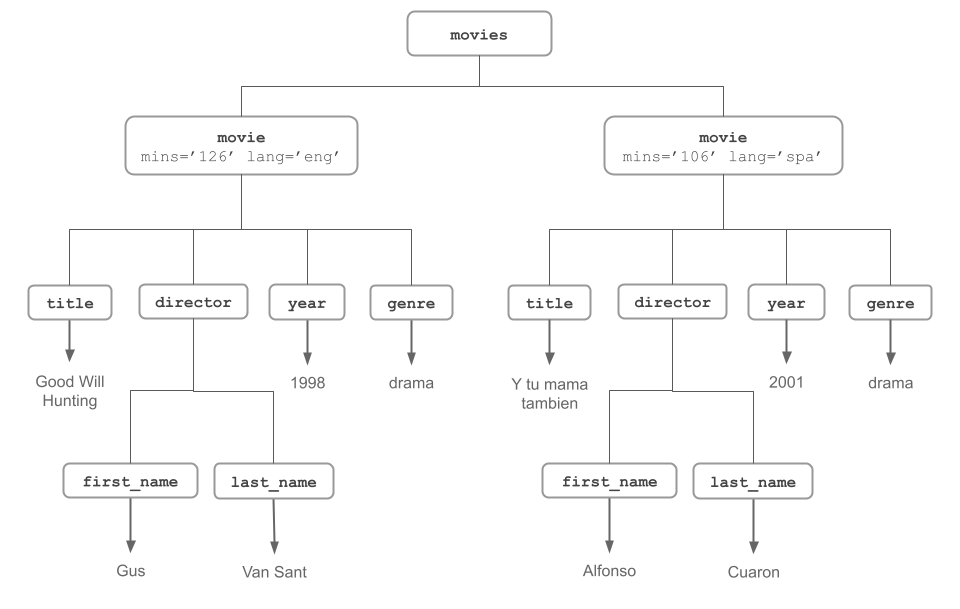
\includegraphics[width=0.85\linewidth]{images/xml/xml-movies-tree1} 

}

\caption{XML movies tree}\label{fig:unnamed-chunk-25}
\end{figure}

Let's create a character vector to store the XML content:

\begin{Shaded}
\begin{Highlighting}[]
\CommentTok{\# toy example with xml string}
\NormalTok{xml\_string }\OtherTok{\textless{}{-}} \FunctionTok{c}\NormalTok{(}
  \StringTok{\textquotesingle{}\textless{}?xml version="1.0" encoding="UTF{-}8"?\textgreater{}\textquotesingle{}}\NormalTok{,}
  \StringTok{\textquotesingle{}\textless{}movies\textgreater{}\textquotesingle{}}\NormalTok{,}
  \StringTok{\textquotesingle{}\textless{}movie mins="126" lang="eng"\textgreater{}\textquotesingle{}}\NormalTok{,}
  \StringTok{\textquotesingle{}\textless{}title\textgreater{}Good Will Hunting\textless{}/title\textgreater{}\textquotesingle{}}\NormalTok{,}
  \StringTok{\textquotesingle{}\textless{}director\textgreater{}\textquotesingle{}}\NormalTok{,}
  \StringTok{\textquotesingle{}\textless{}first\_name\textgreater{}Gus\textless{}/first\_name\textgreater{}\textquotesingle{}}\NormalTok{,}
  \StringTok{\textquotesingle{}\textless{}last\_name\textgreater{}Van Sant\textless{}/last\_name\textgreater{}\textquotesingle{}}\NormalTok{,}
  \StringTok{\textquotesingle{}\textless{}/director\textgreater{}\textquotesingle{}}\NormalTok{,}
  \StringTok{\textquotesingle{}\textless{}year\textgreater{}1998\textless{}/year\textgreater{}\textquotesingle{}}\NormalTok{,}
  \StringTok{\textquotesingle{}\textless{}genre\textgreater{}drama\textless{}/genre\textgreater{}\textquotesingle{}}\NormalTok{,}
  \StringTok{\textquotesingle{}\textless{}/movie\textgreater{}\textquotesingle{}}\NormalTok{,}
  \StringTok{\textquotesingle{}\textless{}movie mins="106" lang="spa"\textgreater{}\textquotesingle{}}\NormalTok{,}
  \StringTok{\textquotesingle{}\textless{}title\textgreater{}Y tu mama tambien\textless{}/title\textgreater{}\textquotesingle{}}\NormalTok{,}
  \StringTok{\textquotesingle{}\textless{}director\textgreater{}\textquotesingle{}}\NormalTok{,}
  \StringTok{\textquotesingle{}\textless{}first\_name\textgreater{}Alfonso\textless{}/first\_name\textgreater{}\textquotesingle{}}\NormalTok{,}
  \StringTok{\textquotesingle{}\textless{}last\_name\textgreater{}Cuaron\textless{}/last\_name\textgreater{}\textquotesingle{}}\NormalTok{,}
  \StringTok{\textquotesingle{}\textless{}/director\textgreater{}\textquotesingle{}}\NormalTok{,}
  \StringTok{\textquotesingle{}\textless{}year\textgreater{}2001\textless{}/year\textgreater{}\textquotesingle{}}\NormalTok{,}
  \StringTok{\textquotesingle{}\textless{}genre\textgreater{}drama\textless{}/genre\textgreater{}\textquotesingle{}}\NormalTok{,}
  \StringTok{\textquotesingle{}\textless{}/movie\textgreater{}\textquotesingle{}}\NormalTok{,}
  \StringTok{\textquotesingle{}\textless{}/movies\textgreater{}\textquotesingle{}}\NormalTok{)}
\end{Highlighting}
\end{Shaded}

Let's parse the content. To do this, we must first create a single contiguous
xml string, which is done with \texttt{paste()} and its \texttt{collapse\ =\ \textquotesingle{}\textquotesingle{}} argument:

\begin{Shaded}
\begin{Highlighting}[]
\CommentTok{\# parsing xml string}
\NormalTok{doc }\OtherTok{\textless{}{-}} \FunctionTok{read\_xml}\NormalTok{(}\FunctionTok{paste}\NormalTok{(xml\_string, }\AttributeTok{collapse =} \StringTok{\textquotesingle{}\textquotesingle{}}\NormalTok{))}

\NormalTok{doc}
\CommentTok{\#\textgreater{} \{xml\_document\}}
\CommentTok{\#\textgreater{} \textless{}movies\textgreater{}}
\CommentTok{\#\textgreater{} [1] \textless{}movie mins="126" lang="eng"\textgreater{}\textbackslash{}n  \textless{}title\textgreater{}Good Will Hunting\textless{}/title\textgreater{}\textbackslash{}n  \textless{}dir ...}
\CommentTok{\#\textgreater{} [2] \textless{}movie mins="106" lang="spa"\textgreater{}\textbackslash{}n  \textless{}title\textgreater{}Y tu mama tambien\textless{}/title\textgreater{}\textbackslash{}n  \textless{}dir ...}
\end{Highlighting}
\end{Shaded}

And let's navigate the tree structure. We begin with \texttt{xml\_root()} to get
access to the root node:

\begin{Shaded}
\begin{Highlighting}[]
\CommentTok{\# root node}
\NormalTok{movies }\OtherTok{\textless{}{-}} \FunctionTok{xml\_root}\NormalTok{(doc)}
\NormalTok{movies}
\CommentTok{\#\textgreater{} \{xml\_document\}}
\CommentTok{\#\textgreater{} \textless{}movies\textgreater{}}
\CommentTok{\#\textgreater{} [1] \textless{}movie mins="126" lang="eng"\textgreater{}\textbackslash{}n  \textless{}title\textgreater{}Good Will Hunting\textless{}/title\textgreater{}\textbackslash{}n  \textless{}dir ...}
\CommentTok{\#\textgreater{} [2] \textless{}movie mins="106" lang="spa"\textgreater{}\textbackslash{}n  \textless{}title\textgreater{}Y tu mama tambien\textless{}/title\textgreater{}\textbackslash{}n  \textless{}dir ...}
\end{Highlighting}
\end{Shaded}

It turns out that \texttt{doc} and \texttt{movies} are actually identical:

\begin{Shaded}
\begin{Highlighting}[]
\FunctionTok{identical}\NormalTok{(doc, movies)}
\CommentTok{\#\textgreater{} [1] TRUE}
\end{Highlighting}
\end{Shaded}

We use the \texttt{xml\_length()} to know how many elements or nodes are in the root
node:

\begin{Shaded}
\begin{Highlighting}[]
\CommentTok{\# parsing xml string}
\FunctionTok{xml\_length}\NormalTok{(doc)}
\CommentTok{\#\textgreater{} [1] 2}
\end{Highlighting}
\end{Shaded}

which confirms what we know about the movies string that contains two \texttt{movie}
elements: one node for ``Good Will Hunting'' and another node for ``Y tu mama
tambien''.

The function \texttt{xml\_children()} allows you to access the children nodes:

\begin{Shaded}
\begin{Highlighting}[]
\FunctionTok{xml\_children}\NormalTok{(doc)}
\CommentTok{\#\textgreater{} \{xml\_nodeset (2)\}}
\CommentTok{\#\textgreater{} [1] \textless{}movie mins="126" lang="eng"\textgreater{}\textbackslash{}n  \textless{}title\textgreater{}Good Will Hunting\textless{}/title\textgreater{}\textbackslash{}n  \textless{}dir ...}
\CommentTok{\#\textgreater{} [2] \textless{}movie mins="106" lang="spa"\textgreater{}\textbackslash{}n  \textless{}title\textgreater{}Y tu mama tambien\textless{}/title\textgreater{}\textbackslash{}n  \textless{}dir ...}
\end{Highlighting}
\end{Shaded}

Notice that the output is an object of class \texttt{"xml\_nodeset"}. To access a
specific node, you use the function \texttt{xml\_child()}. In this example, the node
for movie ``Good Will Hunting'' corresponds to the first node, and we pass this
value to the \texttt{search} argument:

\begin{Shaded}
\begin{Highlighting}[]
\FunctionTok{xml\_child}\NormalTok{(doc, }\AttributeTok{search =} \DecValTok{1}\NormalTok{)}
\CommentTok{\#\textgreater{} \{xml\_node\}}
\CommentTok{\#\textgreater{} \textless{}movie mins="126" lang="eng"\textgreater{}}
\CommentTok{\#\textgreater{} [1] \textless{}title\textgreater{}Good Will Hunting\textless{}/title\textgreater{}}
\CommentTok{\#\textgreater{} [2] \textless{}director\textgreater{}\textbackslash{}n  \textless{}first\_name\textgreater{}Gus\textless{}/first\_name\textgreater{}\textbackslash{}n  \textless{}last\_name\textgreater{}Van Sant\textless{}/last\_n ...}
\CommentTok{\#\textgreater{} [3] \textless{}year\textgreater{}1998\textless{}/year\textgreater{}}
\CommentTok{\#\textgreater{} [4] \textless{}genre\textgreater{}drama\textless{}/genre\textgreater{}}
\end{Highlighting}
\end{Shaded}

Likewise, the second node (``Y tu mama tambien'') is accessed by specifying the
argument \texttt{search\ =\ 2}:

\begin{Shaded}
\begin{Highlighting}[]
\FunctionTok{xml\_child}\NormalTok{(doc, }\AttributeTok{search =} \DecValTok{2}\NormalTok{)}
\CommentTok{\#\textgreater{} \{xml\_node\}}
\CommentTok{\#\textgreater{} \textless{}movie mins="106" lang="spa"\textgreater{}}
\CommentTok{\#\textgreater{} [1] \textless{}title\textgreater{}Y tu mama tambien\textless{}/title\textgreater{}}
\CommentTok{\#\textgreater{} [2] \textless{}director\textgreater{}\textbackslash{}n  \textless{}first\_name\textgreater{}Alfonso\textless{}/first\_name\textgreater{}\textbackslash{}n  \textless{}last\_name\textgreater{}Cuaron\textless{}/last ...}
\CommentTok{\#\textgreater{} [3] \textless{}year\textgreater{}2001\textless{}/year\textgreater{}}
\CommentTok{\#\textgreater{} [4] \textless{}genre\textgreater{}drama\textless{}/genre\textgreater{}}
\end{Highlighting}
\end{Shaded}

This is the view of the tree structure so far:

\begin{figure}

{\centering 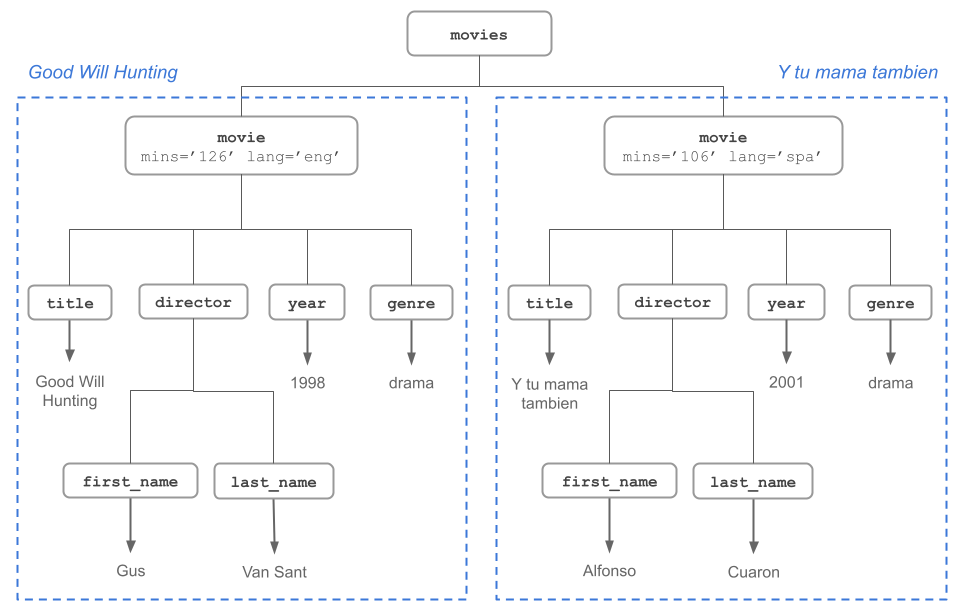
\includegraphics[width=0.85\linewidth]{images/xml/xml-movies-tree2} 

}

\caption{Two movie nodes}\label{fig:unnamed-chunk-34}
\end{figure}

\hypertarget{inspecting-first-node}{%
\subsubsection*{Inspecting first node}\label{inspecting-first-node}}
\addcontentsline{toc}{subsubsection}{Inspecting first node}

Let's go inside the first node, and store the content in the object
\texttt{good\_will}

\begin{Shaded}
\begin{Highlighting}[]
\CommentTok{\# first child}
\NormalTok{good\_will }\OtherTok{\textless{}{-}} \FunctionTok{xml\_child}\NormalTok{(doc, }\AttributeTok{search =} \DecValTok{1}\NormalTok{)}
\NormalTok{good\_will}
\CommentTok{\#\textgreater{} \{xml\_node\}}
\CommentTok{\#\textgreater{} \textless{}movie mins="126" lang="eng"\textgreater{}}
\CommentTok{\#\textgreater{} [1] \textless{}title\textgreater{}Good Will Hunting\textless{}/title\textgreater{}}
\CommentTok{\#\textgreater{} [2] \textless{}director\textgreater{}\textbackslash{}n  \textless{}first\_name\textgreater{}Gus\textless{}/first\_name\textgreater{}\textbackslash{}n  \textless{}last\_name\textgreater{}Van Sant\textless{}/last\_n ...}
\CommentTok{\#\textgreater{} [3] \textless{}year\textgreater{}1998\textless{}/year\textgreater{}}
\CommentTok{\#\textgreater{} [4] \textless{}genre\textgreater{}drama\textless{}/genre\textgreater{}}
\end{Highlighting}
\end{Shaded}

and let's do the same for the second node, storing the content in the object
\texttt{tu\_mama}:

\begin{Shaded}
\begin{Highlighting}[]
\CommentTok{\# second child}
\NormalTok{tu\_mama }\OtherTok{\textless{}{-}} \FunctionTok{xml\_child}\NormalTok{(doc, }\AttributeTok{search =} \DecValTok{2}\NormalTok{)}
\NormalTok{tu\_mama}
\CommentTok{\#\textgreater{} \{xml\_node\}}
\CommentTok{\#\textgreater{} \textless{}movie mins="106" lang="spa"\textgreater{}}
\CommentTok{\#\textgreater{} [1] \textless{}title\textgreater{}Y tu mama tambien\textless{}/title\textgreater{}}
\CommentTok{\#\textgreater{} [2] \textless{}director\textgreater{}\textbackslash{}n  \textless{}first\_name\textgreater{}Alfonso\textless{}/first\_name\textgreater{}\textbackslash{}n  \textless{}last\_name\textgreater{}Cuaron\textless{}/last ...}
\CommentTok{\#\textgreater{} [3] \textless{}year\textgreater{}2001\textless{}/year\textgreater{}}
\CommentTok{\#\textgreater{} [4] \textless{}genre\textgreater{}drama\textless{}/genre\textgreater{}}
\end{Highlighting}
\end{Shaded}

We can then again apply \texttt{xml\_children()} on each node to see what children
nodes \texttt{good\_will} and \texttt{tu\_mama} have:

\begin{Shaded}
\begin{Highlighting}[]
\CommentTok{\# children of good\_will}
\FunctionTok{xml\_children}\NormalTok{(good\_will)}
\CommentTok{\#\textgreater{} \{xml\_nodeset (4)\}}
\CommentTok{\#\textgreater{} [1] \textless{}title\textgreater{}Good Will Hunting\textless{}/title\textgreater{}}
\CommentTok{\#\textgreater{} [2] \textless{}director\textgreater{}\textbackslash{}n  \textless{}first\_name\textgreater{}Gus\textless{}/first\_name\textgreater{}\textbackslash{}n  \textless{}last\_name\textgreater{}Van Sant\textless{}/last\_n ...}
\CommentTok{\#\textgreater{} [3] \textless{}year\textgreater{}1998\textless{}/year\textgreater{}}
\CommentTok{\#\textgreater{} [4] \textless{}genre\textgreater{}drama\textless{}/genre\textgreater{}}
\end{Highlighting}
\end{Shaded}

\begin{Shaded}
\begin{Highlighting}[]
\CommentTok{\# children of tu\_mama}
\FunctionTok{xml\_children}\NormalTok{(tu\_mama)}
\CommentTok{\#\textgreater{} \{xml\_nodeset (4)\}}
\CommentTok{\#\textgreater{} [1] \textless{}title\textgreater{}Y tu mama tambien\textless{}/title\textgreater{}}
\CommentTok{\#\textgreater{} [2] \textless{}director\textgreater{}\textbackslash{}n  \textless{}first\_name\textgreater{}Alfonso\textless{}/first\_name\textgreater{}\textbackslash{}n  \textless{}last\_name\textgreater{}Cuaron\textless{}/last ...}
\CommentTok{\#\textgreater{} [3] \textless{}year\textgreater{}2001\textless{}/year\textgreater{}}
\CommentTok{\#\textgreater{} [4] \textless{}genre\textgreater{}drama\textless{}/genre\textgreater{}}
\end{Highlighting}
\end{Shaded}

The visual diagram for \texttt{good\_will} depicts the four nodes:

\begin{figure}

{\centering 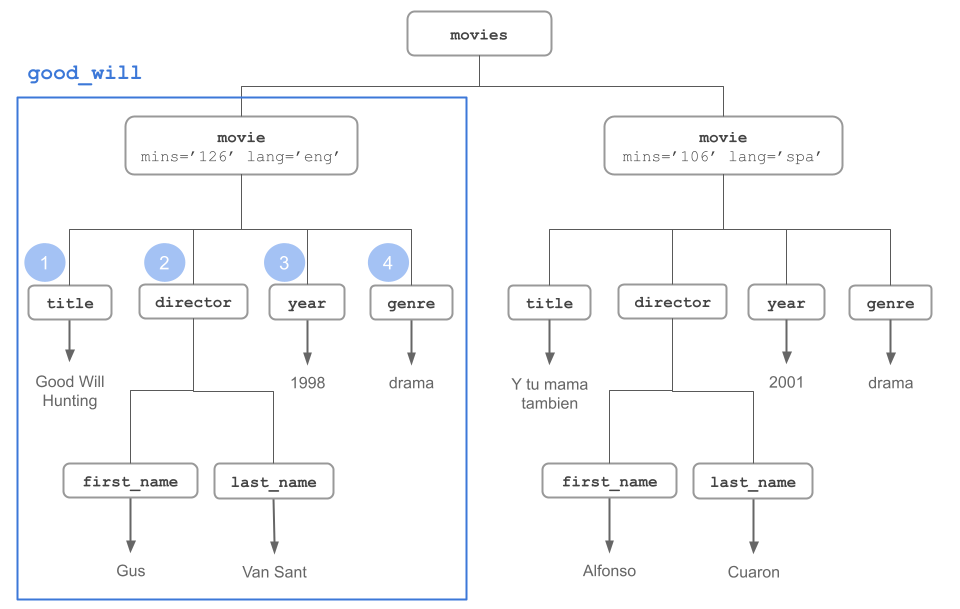
\includegraphics[width=0.85\linewidth]{images/xml/xml-movies-tree3} 

}

\caption{Children nodes of 'Good Will Hunting'}\label{fig:unnamed-chunk-39}
\end{figure}

The code below shows a deeper inspection of \texttt{good\_will}. The function
\texttt{xml\_name()} gives the name of a node.

\begin{Shaded}
\begin{Highlighting}[]
\CommentTok{\# name of an element}
\FunctionTok{xml\_name}\NormalTok{(good\_will)}
\CommentTok{\#\textgreater{} [1] "movie"}
\end{Highlighting}
\end{Shaded}

The function \texttt{xml\_attrs()} gives you the attributes of a node. In this case,
the node of \texttt{good\_will} has to attributes \texttt{"mins"} and \texttt{"lang"}

\begin{Shaded}
\begin{Highlighting}[]
\CommentTok{\# attributes}
\FunctionTok{xml\_attrs}\NormalTok{(good\_will)}
\CommentTok{\#\textgreater{}  mins  lang }
\CommentTok{\#\textgreater{} "126" "eng"}
\end{Highlighting}
\end{Shaded}

As we previously saw, \texttt{xml\_length()} gives the number of children nodes inside
a given node:

\begin{Shaded}
\begin{Highlighting}[]
\CommentTok{\# how many children}
\FunctionTok{xml\_length}\NormalTok{(good\_will)}
\CommentTok{\#\textgreater{} [1] 4}
\end{Highlighting}
\end{Shaded}

Likewise, we can move along the children nodes, and find information about
their names, their subchildren, and so on:

\begin{Shaded}
\begin{Highlighting}[]
\CommentTok{\# name of children (of good\_will)}
\FunctionTok{xml\_name}\NormalTok{(}\FunctionTok{xml\_children}\NormalTok{(good\_will))}
\CommentTok{\#\textgreater{} [1] "title"    "director" "year"     "genre"}

\CommentTok{\# good\_will title}
\FunctionTok{xml\_child}\NormalTok{(good\_will, }\StringTok{"title"}\NormalTok{)}
\CommentTok{\#\textgreater{} \{xml\_node\}}
\CommentTok{\#\textgreater{} \textless{}title\textgreater{}}
\end{Highlighting}
\end{Shaded}

\begin{Shaded}
\begin{Highlighting}[]
\CommentTok{\# good\_will title}
\NormalTok{title1 }\OtherTok{\textless{}{-}} \FunctionTok{xml\_child}\NormalTok{(good\_will, }\StringTok{"title"}\NormalTok{)}
\NormalTok{title1}
\CommentTok{\#\textgreater{} \{xml\_node\}}
\CommentTok{\#\textgreater{} \textless{}title\textgreater{}}

\CommentTok{\# content good\_will title}
\FunctionTok{xml\_contents}\NormalTok{(title1)}
\CommentTok{\#\textgreater{} \{xml\_nodeset (1)\}}
\CommentTok{\#\textgreater{} [1] Good Will Hunting}

\CommentTok{\# text good\_will title}
\FunctionTok{xml\_text}\NormalTok{(title1)}
\CommentTok{\#\textgreater{} [1] "Good Will Hunting"}
\end{Highlighting}
\end{Shaded}

\hypertarget{inspecting-director-node}{%
\subsubsection{Inspecting director node}\label{inspecting-director-node}}

\begin{Shaded}
\begin{Highlighting}[]
\CommentTok{\# good\_will director}
\NormalTok{dir1 }\OtherTok{\textless{}{-}} \FunctionTok{xml\_child}\NormalTok{(good\_will, }\StringTok{"director"}\NormalTok{)}
\NormalTok{dir1}
\CommentTok{\#\textgreater{} \{xml\_node\}}
\CommentTok{\#\textgreater{} \textless{}director\textgreater{}}
\CommentTok{\#\textgreater{} [1] \textless{}first\_name\textgreater{}Gus\textless{}/first\_name\textgreater{}}
\CommentTok{\#\textgreater{} [2] \textless{}last\_name\textgreater{}Van Sant\textless{}/last\_name\textgreater{}}
\end{Highlighting}
\end{Shaded}

\begin{Shaded}
\begin{Highlighting}[]
\FunctionTok{xml\_children}\NormalTok{(dir1)}
\CommentTok{\#\textgreater{} \{xml\_nodeset (2)\}}
\CommentTok{\#\textgreater{} [1] \textless{}first\_name\textgreater{}Gus\textless{}/first\_name\textgreater{}}
\CommentTok{\#\textgreater{} [2] \textless{}last\_name\textgreater{}Van Sant\textless{}/last\_name\textgreater{}}
\end{Highlighting}
\end{Shaded}

To extract just the text, we use \texttt{xml\_text()}:

\begin{Shaded}
\begin{Highlighting}[]
\FunctionTok{xml\_text}\NormalTok{(dir1)}
\CommentTok{\#\textgreater{} [1] "GusVan Sant"}
\end{Highlighting}
\end{Shaded}

The visual diagram for \texttt{good\_will} with its director node is depicted in this
figure:

\begin{figure}

{\centering 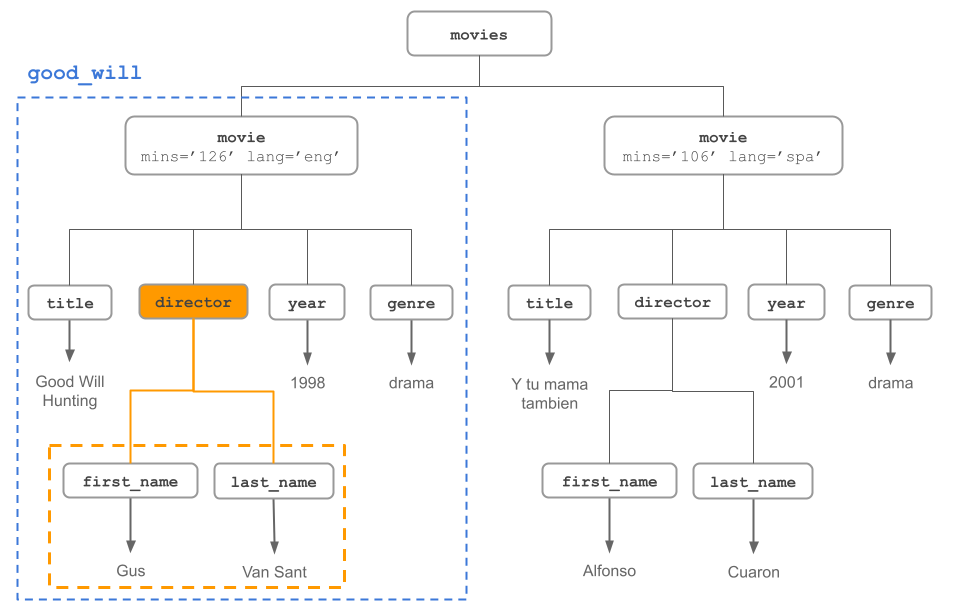
\includegraphics[width=0.85\linewidth]{images/xml/xml-movies-tree4} 

}

\caption{Director node of 'Good Will Hunting'}\label{fig:unnamed-chunk-48}
\end{figure}

\hypertarget{xpath}{%
\chapter{XPath Language}\label{xpath}}

In the preceding chapter you learned about the main functions in \texttt{"xml"} that
allows us to parse XML and HTML documents. While those functions can be quite
useful to navigate through the elements of an XML document, their default usage
can be a bit limiting.

The real parsing power comes from the ability to
\textbf{locate nodes and extract information from them}. For this, we need to be
able to perform queries on the parsed content. The solution is provided by
\textbf{XPath}, which is a language to navigate through elements and attributes in
an XML/HTML document.

\hypertarget{what-is-xpath}{%
\section{What is XPath?}\label{what-is-xpath}}

XPath is a language for finding information in an XML document. It works by
identifying patterns to match data or content. To be more precise, XPath uses
\textbf{path expressions} to select nodes in an XML document by taking into account
the tree structure of XML based on:

\begin{itemize}
\item
  node names
\item
  node content
\item
  a node's relationship to other nodes
\end{itemize}

\hypertarget{xpath-syntax}{%
\subsection{XPath Syntax}\label{xpath-syntax}}

The key concept is knowing how to write XPath expressions. XPath expressions
have a syntax similar to the way files are located in a hierarchy of directories
and folders in a computer file system. For instance:

\begin{verbatim}
/movies/movie
\end{verbatim}

is the XPath expression to locate the \texttt{movie} children in the \texttt{movies} (root)
element

\hypertarget{selecting-nodes}{%
\subsection{Selecting Nodes}\label{selecting-nodes}}

The main symbols to define path expressions are:

\begin{longtable}[]{@{}ll@{}}
\toprule\noalign{}
Symbol & Description \\
\midrule\noalign{}
\endhead
\bottomrule\noalign{}
\endlastfoot
\texttt{/} & selects from the root node \\
\texttt{//} & selects nodes anywhere \\
\texttt{.} & selects the current node \\
\texttt{..} & selects the parent of the current node \\
\texttt{@} & selects attributes \\
\texttt{{[}{]}} & square brackets to indicate attributes \\
\texttt{*} & matches any element node \\
\texttt{@*} & matches any attribute node \\
\end{longtable}

For instance:

\begin{longtable}[]{@{}
  >{\raggedright\arraybackslash}p{(\columnwidth - 2\tabcolsep) * \real{0.3492}}
  >{\raggedright\arraybackslash}p{(\columnwidth - 2\tabcolsep) * \real{0.6508}}@{}}
\toprule\noalign{}
\begin{minipage}[b]{\linewidth}\raggedright
Example
\end{minipage} & \begin{minipage}[b]{\linewidth}\raggedright
Description
\end{minipage} \\
\midrule\noalign{}
\endhead
\bottomrule\noalign{}
\endlastfoot
\texttt{/node} & selects top level node \\
\texttt{//node} & selects nodes at any level \\
\texttt{node{[}@attr{]}} & node that has an attribute named \texttt{attr} \\
\texttt{node{[}@attr="abc"{]}} & node that has an attribute named \texttt{attr} with value \texttt{"abc"} \\
\texttt{node/@attr} & value of an attribute \texttt{attr} in node with such attribute \\
\texttt{node/*} & any (child) element in node \\
\texttt{node/@*} & value of any attribute in node \\
\end{longtable}

\hypertarget{xpath-examples}{%
\section{XPath Examples}\label{xpath-examples}}

To make things less abstract, let's bring back the \texttt{movies} XML document
containing two movies \emph{Good Will Hunting} and \emph{Y tu mama tambien}

\begin{figure}

{\centering 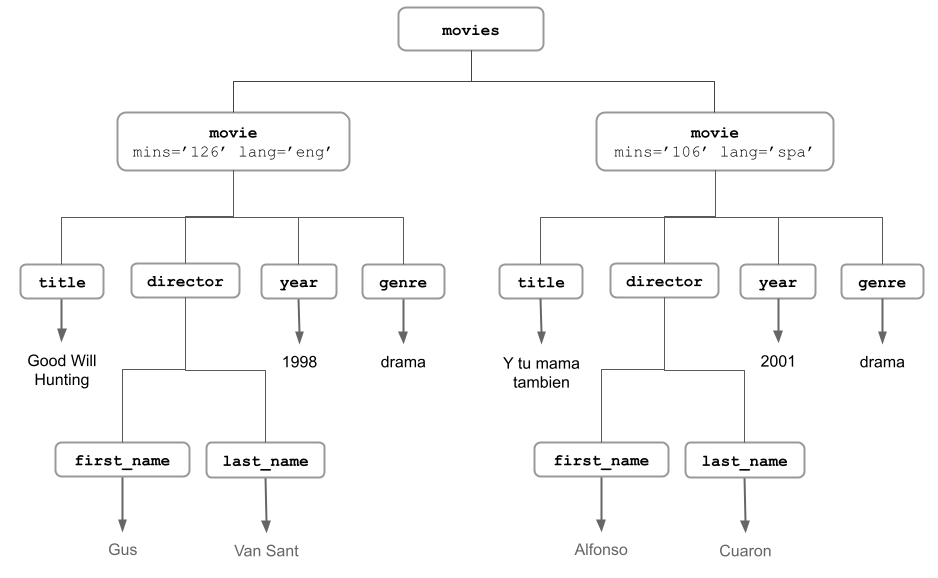
\includegraphics[width=0.85\linewidth]{images/xpath/xpath-example0} 

}

\caption{XML movies}\label{fig:unnamed-chunk-50}
\end{figure}

The following diagrams illustrate different XPath expressions to match and
select nodes based on either: their names, their content, or their relationship
to other nodes.

\begin{figure}

{\centering 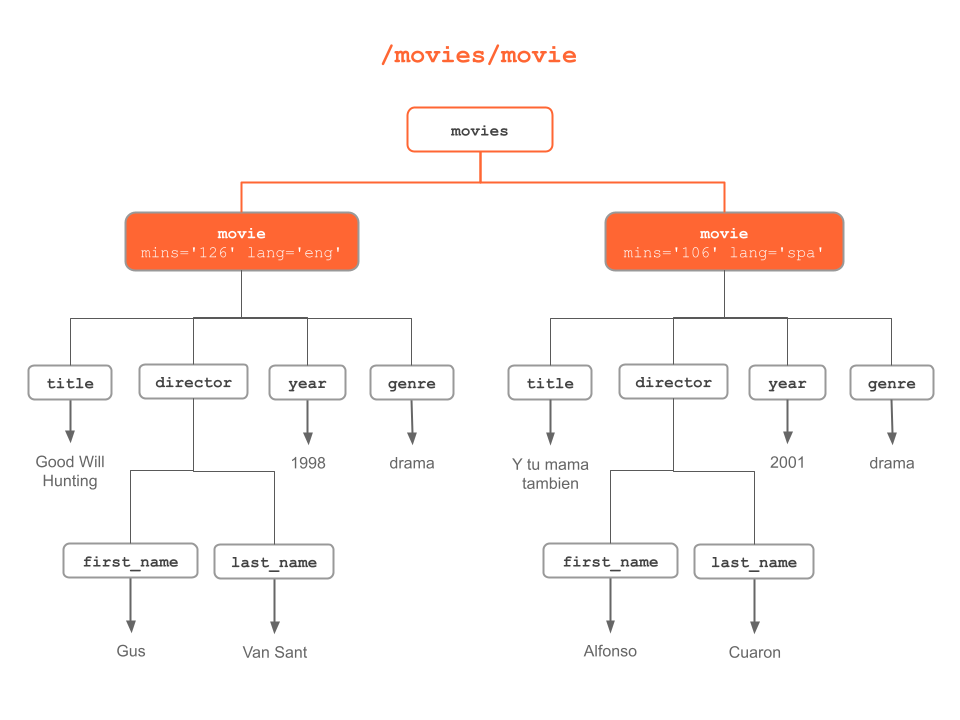
\includegraphics[width=0.85\linewidth]{images/xpath/xpath-example1} 

}

\caption{"movie" nodes}\label{fig:unnamed-chunk-51}
\end{figure}

\begin{figure}

{\centering 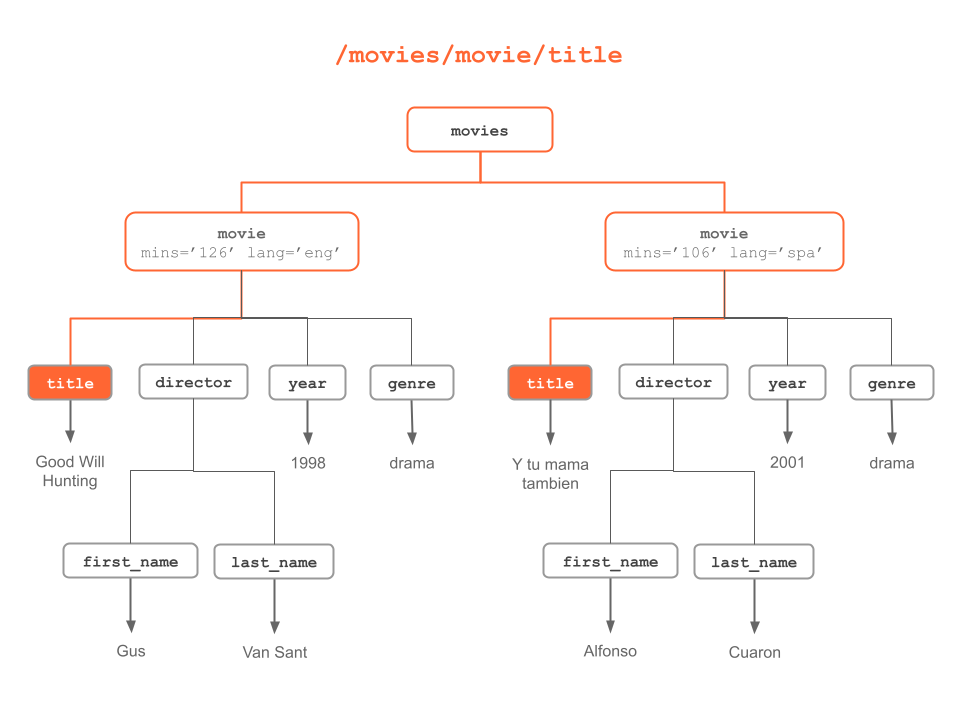
\includegraphics[width=0.85\linewidth]{images/xpath/xpath-example2} 

}

\caption{"title" nodes}\label{fig:unnamed-chunk-52}
\end{figure}

\begin{figure}

{\centering 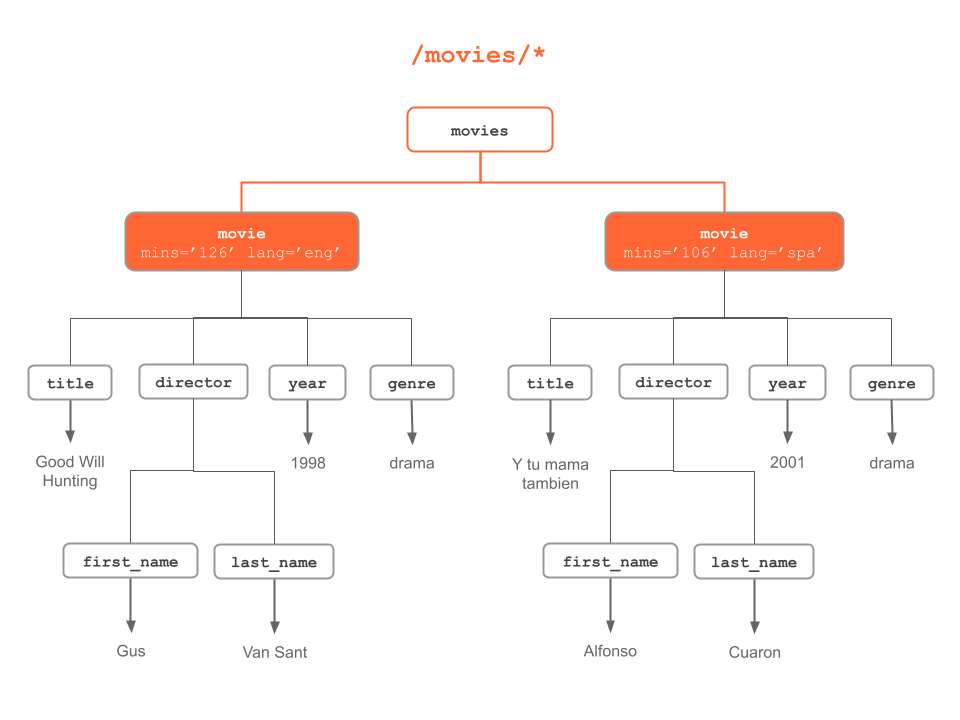
\includegraphics[width=0.85\linewidth]{images/xpath/xpath-example3} 

}

\caption{Any nodes of "movies" node}\label{fig:unnamed-chunk-53}
\end{figure}

\begin{figure}

{\centering 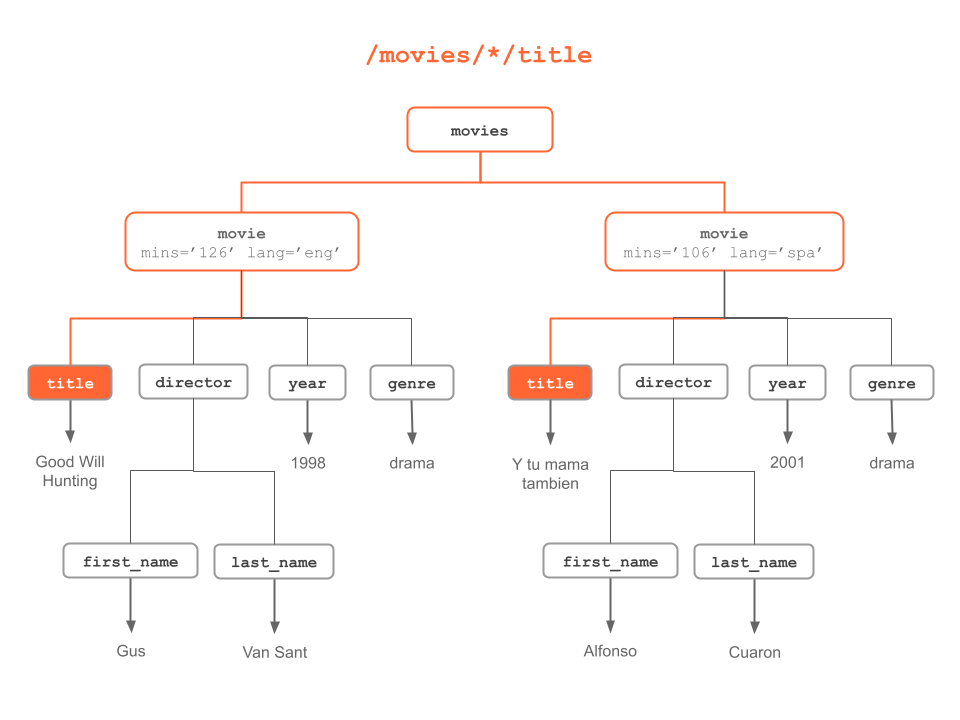
\includegraphics[width=0.85\linewidth]{images/xpath/xpath-example4} 

}

\caption{Another way to select "title" nodes}\label{fig:unnamed-chunk-54}
\end{figure}

\begin{figure}

{\centering 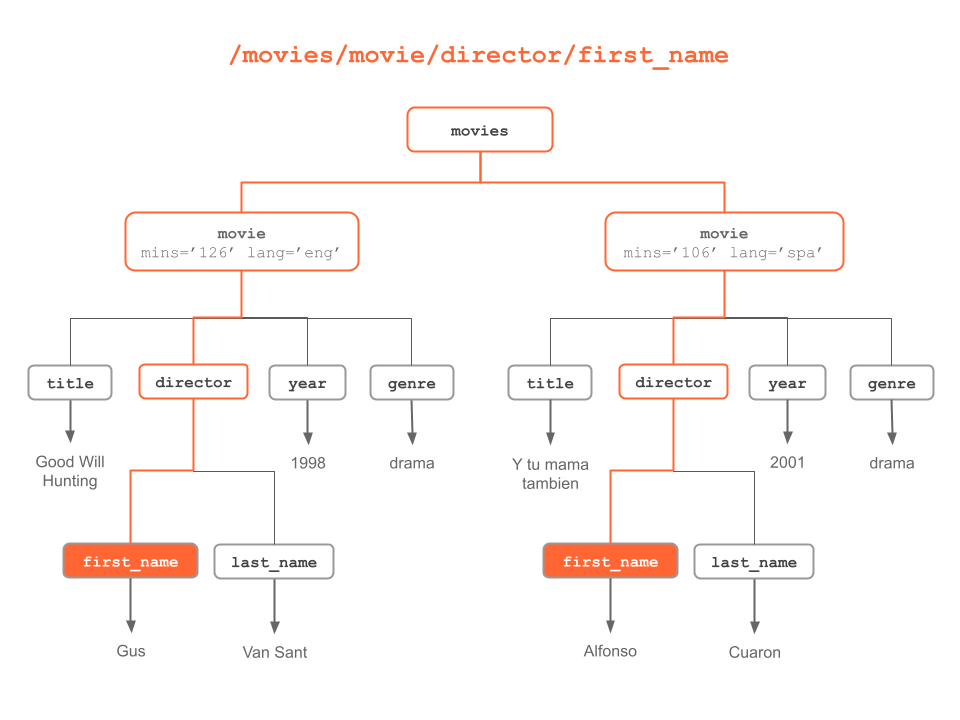
\includegraphics[width=0.85\linewidth]{images/xpath/xpath-example5} 

}

\caption{"first name" nodes}\label{fig:unnamed-chunk-55}
\end{figure}

\begin{figure}

{\centering 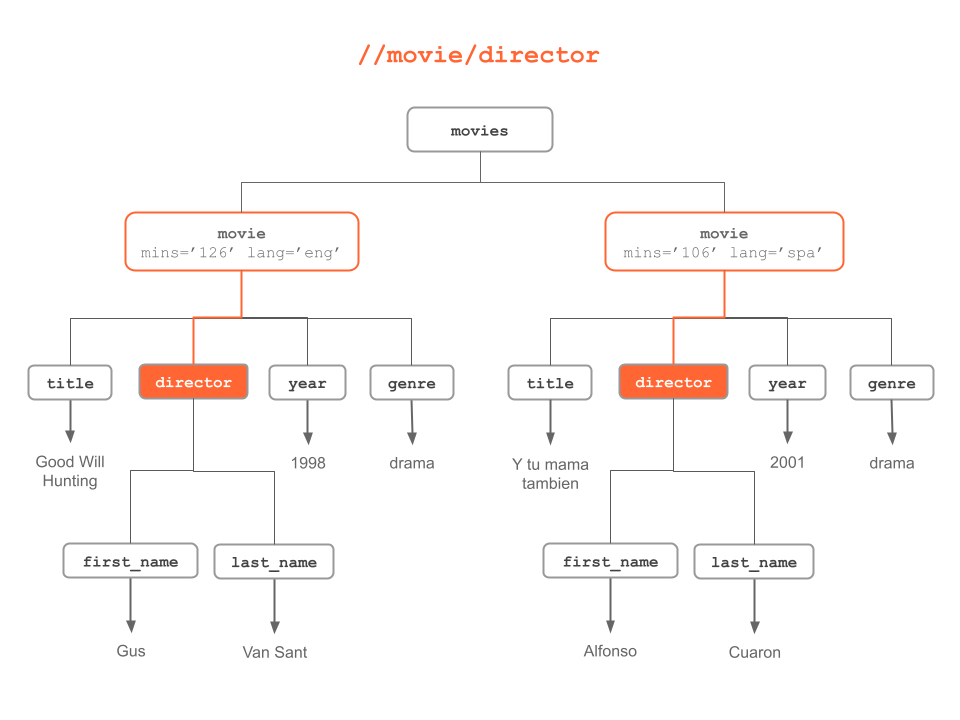
\includegraphics[width=0.85\linewidth]{images/xpath/xpath-example6} 

}

\caption{"movie/director" anywhere in the XML tree}\label{fig:unnamed-chunk-56}
\end{figure}

\begin{figure}

{\centering 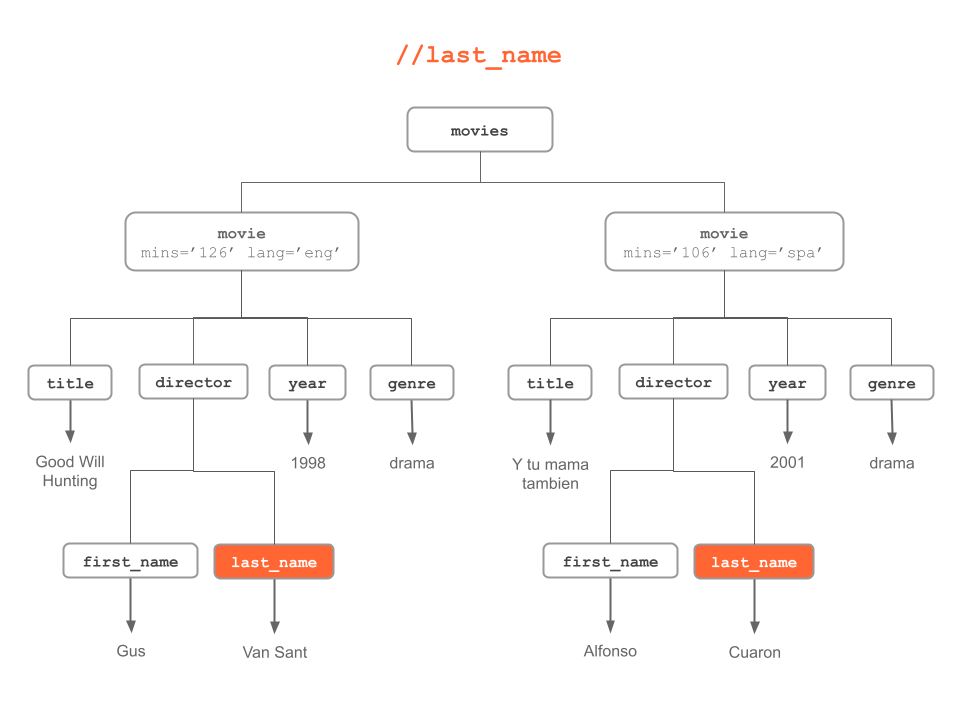
\includegraphics[width=0.85\linewidth]{images/xpath/xpath-example7} 

}

\caption{"last name" nodes anywhere in the XML tree}\label{fig:unnamed-chunk-57}
\end{figure}

\begin{figure}

{\centering 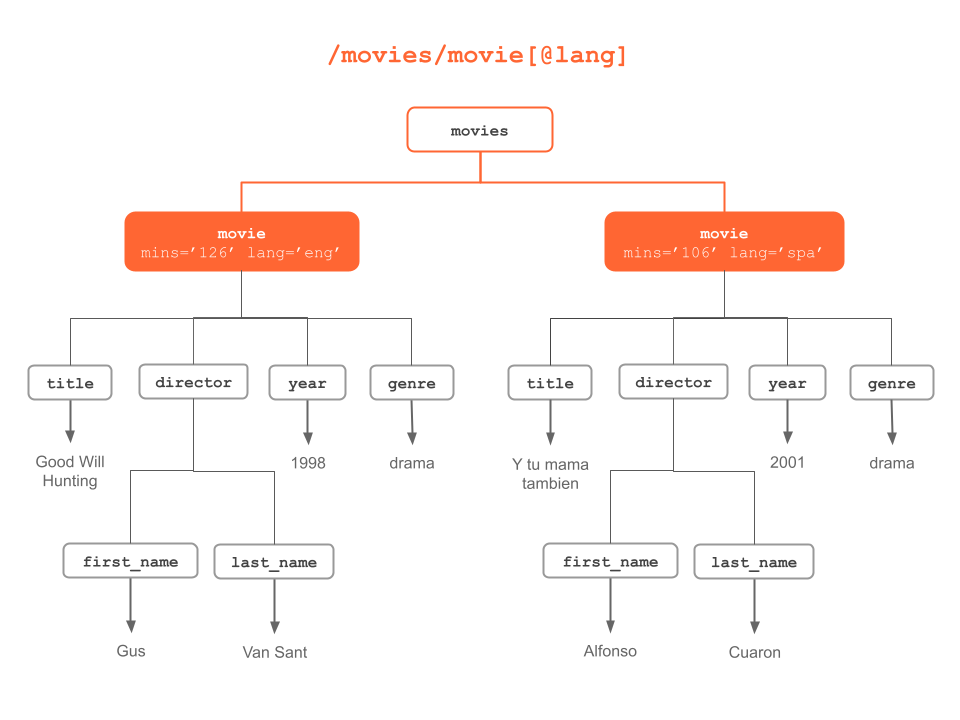
\includegraphics[width=0.85\linewidth]{images/xpath/xpath-example8} 

}

\caption{"movie" nodes having "lang" attribute}\label{fig:unnamed-chunk-58}
\end{figure}

\begin{figure}

{\centering 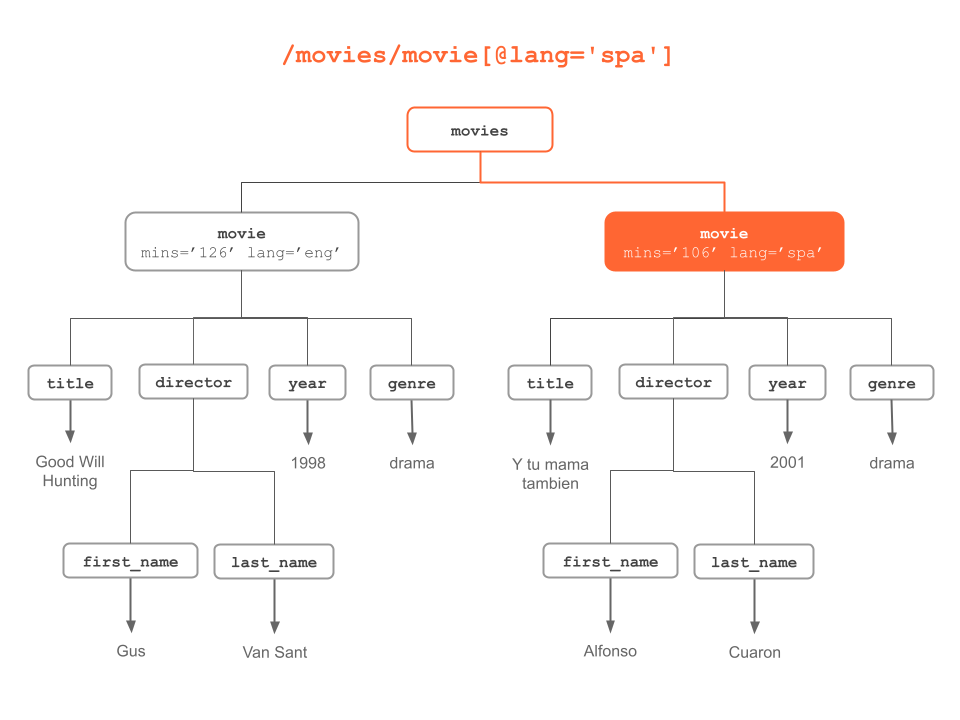
\includegraphics[width=0.85\linewidth]{images/xpath/xpath-example9} 

}

\caption{"movie" nodes with "lang" attribute having value "spa"}\label{fig:unnamed-chunk-59}
\end{figure}

\begin{figure}

{\centering 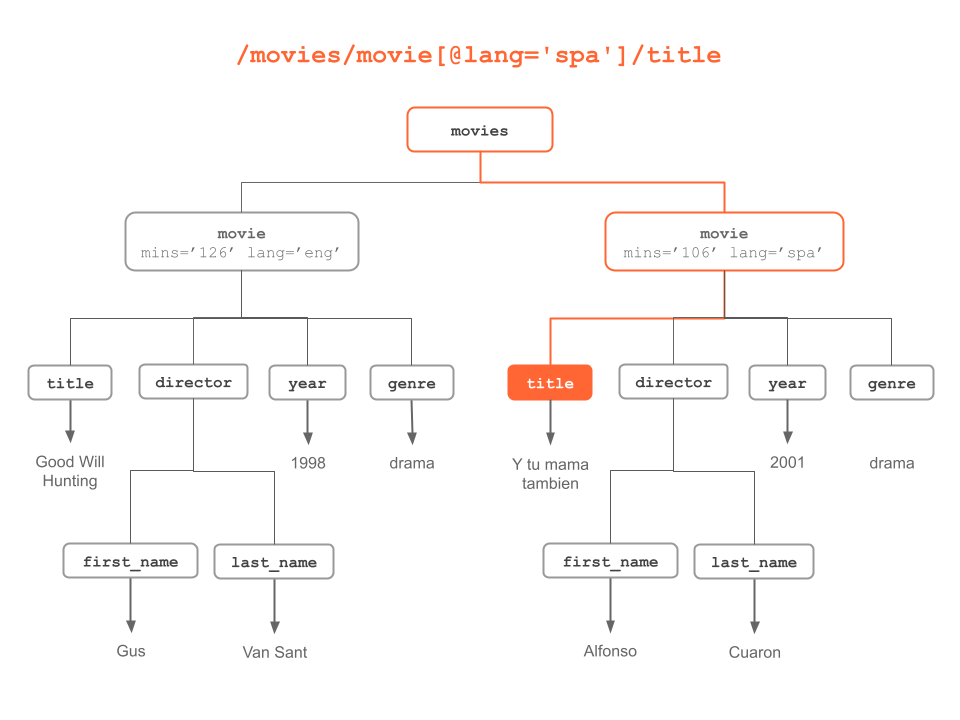
\includegraphics[width=0.85\linewidth]{images/xpath/xpath-example10} 

}

\caption{"title" node of movie with spanish language attribute}\label{fig:unnamed-chunk-60}
\end{figure}

\begin{figure}

{\centering 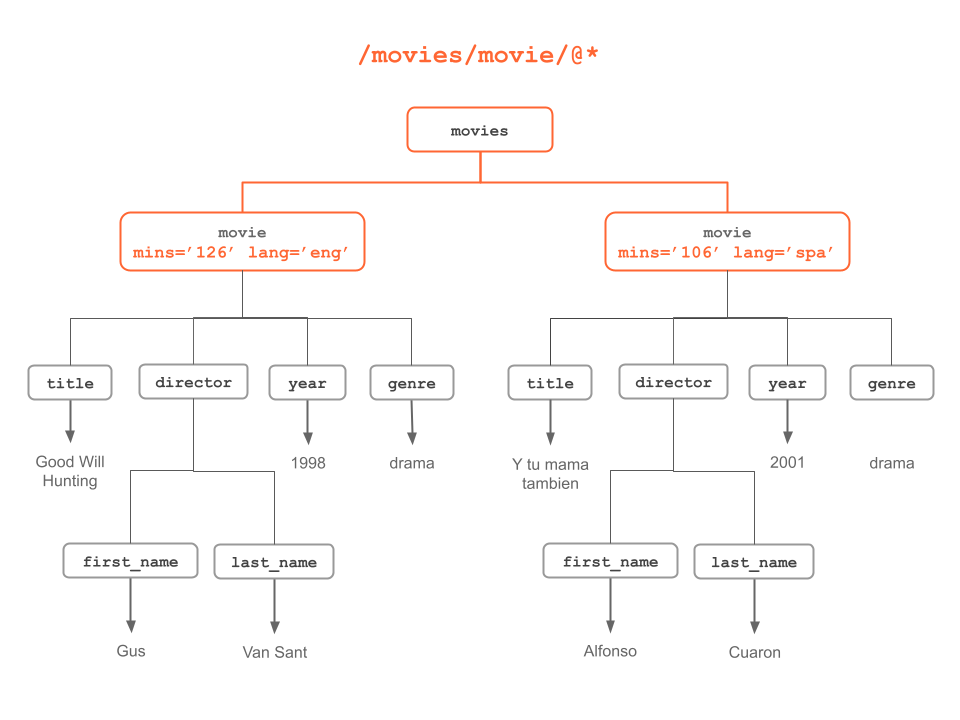
\includegraphics[width=0.85\linewidth]{images/xpath/xpath-example11} 

}

\caption{Any atrribute of "movie" nodes}\label{fig:unnamed-chunk-61}
\end{figure}

\hypertarget{using-xpath-functions}{%
\section{Using XPath Functions}\label{using-xpath-functions}}

The R package \texttt{"xml2"} provides a large number of functions that admit
XPath expressions; these functions have the \texttt{xpath} argument. The following
code snippets, based on the above pattern examples, show you how to use
some of these functions.

\begin{Shaded}
\begin{Highlighting}[]
\CommentTok{\# toy example with xml string}
\NormalTok{xml\_string }\OtherTok{\textless{}{-}} \FunctionTok{c}\NormalTok{(}
  \StringTok{\textquotesingle{}\textless{}?xml version="1.0" encoding="UTF{-}8"?\textgreater{}\textquotesingle{}}\NormalTok{,}
  \StringTok{\textquotesingle{}\textless{}movies\textgreater{}\textquotesingle{}}\NormalTok{,}
  \StringTok{\textquotesingle{}\textless{}movie mins="126" lang="eng"\textgreater{}\textquotesingle{}}\NormalTok{,}
  \StringTok{\textquotesingle{}\textless{}title\textgreater{}Good Will Hunting\textless{}/title\textgreater{}\textquotesingle{}}\NormalTok{,}
  \StringTok{\textquotesingle{}\textless{}director\textgreater{}\textquotesingle{}}\NormalTok{,}
  \StringTok{\textquotesingle{}\textless{}first\_name\textgreater{}Gus\textless{}/first\_name\textgreater{}\textquotesingle{}}\NormalTok{,}
  \StringTok{\textquotesingle{}\textless{}last\_name\textgreater{}Van Sant\textless{}/last\_name\textgreater{}\textquotesingle{}}\NormalTok{,}
  \StringTok{\textquotesingle{}\textless{}/director\textgreater{}\textquotesingle{}}\NormalTok{,}
  \StringTok{\textquotesingle{}\textless{}year\textgreater{}1998\textless{}/year\textgreater{}\textquotesingle{}}\NormalTok{,}
  \StringTok{\textquotesingle{}\textless{}genre\textgreater{}drama\textless{}/genre\textgreater{}\textquotesingle{}}\NormalTok{,}
  \StringTok{\textquotesingle{}\textless{}/movie\textgreater{}\textquotesingle{}}\NormalTok{,}
  \StringTok{\textquotesingle{}\textless{}movie mins="106" lang="spa"\textgreater{}\textquotesingle{}}\NormalTok{,}
  \StringTok{\textquotesingle{}\textless{}title\textgreater{}Y tu mama tambien\textless{}/title\textgreater{}\textquotesingle{}}\NormalTok{,}
  \StringTok{\textquotesingle{}\textless{}director\textgreater{}\textquotesingle{}}\NormalTok{,}
  \StringTok{\textquotesingle{}\textless{}first\_name\textgreater{}Alfonso\textless{}/first\_name\textgreater{}\textquotesingle{}}\NormalTok{,}
  \StringTok{\textquotesingle{}\textless{}last\_name\textgreater{}Cuaron\textless{}/last\_name\textgreater{}\textquotesingle{}}\NormalTok{,}
  \StringTok{\textquotesingle{}\textless{}/director\textgreater{}\textquotesingle{}}\NormalTok{,}
  \StringTok{\textquotesingle{}\textless{}year\textgreater{}2001\textless{}/year\textgreater{}\textquotesingle{}}\NormalTok{,}
  \StringTok{\textquotesingle{}\textless{}genre\textgreater{}drama\textless{}/genre\textgreater{}\textquotesingle{}}\NormalTok{,}
  \StringTok{\textquotesingle{}\textless{}/movie\textgreater{}\textquotesingle{}}\NormalTok{,}
  \StringTok{\textquotesingle{}\textless{}/movies\textgreater{}\textquotesingle{}}\NormalTok{)}

\CommentTok{\# parsing xml string}
\NormalTok{doc }\OtherTok{=} \FunctionTok{read\_xml}\NormalTok{(}\FunctionTok{paste}\NormalTok{(xml\_string, }\AttributeTok{collapse =} \StringTok{\textquotesingle{}\textquotesingle{}}\NormalTok{))}
\end{Highlighting}
\end{Shaded}

\begin{Shaded}
\begin{Highlighting}[]
\CommentTok{\# movie children (from root node)}
\NormalTok{movie\_nodes }\OtherTok{=} \FunctionTok{xml\_find\_all}\NormalTok{(doc, }\AttributeTok{xpath =} \StringTok{"/movies/movie"}\NormalTok{)}
\NormalTok{movie\_nodes}
\CommentTok{\#\textgreater{} \{xml\_nodeset (2)\}}
\CommentTok{\#\textgreater{} [1] \textless{}movie mins="126" lang="eng"\textgreater{}\textbackslash{}n  \textless{}title\textgreater{}Good Will Hunting\textless{}/title\textgreater{}\textbackslash{}n  \textless{}dir ...}
\CommentTok{\#\textgreater{} [2] \textless{}movie mins="106" lang="spa"\textgreater{}\textbackslash{}n  \textless{}title\textgreater{}Y tu mama tambien\textless{}/title\textgreater{}\textbackslash{}n  \textless{}dir ...}
\end{Highlighting}
\end{Shaded}

\begin{Shaded}
\begin{Highlighting}[]
\CommentTok{\# title children (from root node)}
\NormalTok{title\_nodes }\OtherTok{=} \FunctionTok{xml\_find\_all}\NormalTok{(doc, }\AttributeTok{xpath =} \StringTok{"/movies/movie/title"}\NormalTok{)}
\NormalTok{title\_nodes}
\CommentTok{\#\textgreater{} \{xml\_nodeset (2)\}}
\CommentTok{\#\textgreater{} [1] \textless{}title\textgreater{}Good Will Hunting\textless{}/title\textgreater{}}
\CommentTok{\#\textgreater{} [2] \textless{}title\textgreater{}Y tu mama tambien\textless{}/title\textgreater{}}
\end{Highlighting}
\end{Shaded}

\begin{Shaded}
\begin{Highlighting}[]
\CommentTok{\# text content of title\_nodes}
\FunctionTok{xml\_text}\NormalTok{(title\_nodes)}
\CommentTok{\#\textgreater{} [1] "Good Will Hunting" "Y tu mama tambien"}
\end{Highlighting}
\end{Shaded}

\begin{Shaded}
\begin{Highlighting}[]
\CommentTok{\# director children (from any movie element)}
\NormalTok{director\_nodes }\OtherTok{=} \FunctionTok{xml\_find\_all}\NormalTok{(doc, }\StringTok{"//movie/director"}\NormalTok{)}
\NormalTok{director\_nodes}
\CommentTok{\#\textgreater{} \{xml\_nodeset (2)\}}
\CommentTok{\#\textgreater{} [1] \textless{}director\textgreater{}\textbackslash{}n  \textless{}first\_name\textgreater{}Gus\textless{}/first\_name\textgreater{}\textbackslash{}n  \textless{}last\_name\textgreater{}Van Sant\textless{}/last\_n ...}
\CommentTok{\#\textgreater{} [2] \textless{}director\textgreater{}\textbackslash{}n  \textless{}first\_name\textgreater{}Alfonso\textless{}/first\_name\textgreater{}\textbackslash{}n  \textless{}last\_name\textgreater{}Cuaron\textless{}/last ...}
\end{Highlighting}
\end{Shaded}

\begin{Shaded}
\begin{Highlighting}[]
\CommentTok{\# text content of director\_nodes}
\FunctionTok{xml\_text}\NormalTok{(director\_nodes)}
\CommentTok{\#\textgreater{} [1] "GusVan Sant"   "AlfonsoCuaron"}
\end{Highlighting}
\end{Shaded}

\begin{Shaded}
\begin{Highlighting}[]
\CommentTok{\# last\_name (from anywhere in the tree)}
\NormalTok{last\_name\_nodes }\OtherTok{=} \FunctionTok{xml\_find\_all}\NormalTok{(doc, }\StringTok{"//last\_name"}\NormalTok{)}
\NormalTok{last\_name\_nodes}
\CommentTok{\#\textgreater{} \{xml\_nodeset (2)\}}
\CommentTok{\#\textgreater{} [1] \textless{}last\_name\textgreater{}Van Sant\textless{}/last\_name\textgreater{}}
\CommentTok{\#\textgreater{} [2] \textless{}last\_name\textgreater{}Cuaron\textless{}/last\_name\textgreater{}}
\end{Highlighting}
\end{Shaded}

\begin{Shaded}
\begin{Highlighting}[]
\CommentTok{\# text of last\_name (from anywhere in the tree)}
\FunctionTok{xml\_text}\NormalTok{(last\_name\_nodes)}
\CommentTok{\#\textgreater{} [1] "Van Sant" "Cuaron"}
\end{Highlighting}
\end{Shaded}

\begin{Shaded}
\begin{Highlighting}[]
\CommentTok{\# title node of movie with attribute lang=\textquotesingle{}spa\textquotesingle{}}
\NormalTok{title\_spa }\OtherTok{=} \FunctionTok{xml\_find\_all}\NormalTok{(doc, }\StringTok{"/movies/movie[@lang=\textquotesingle{}spa\textquotesingle{}]/title"}\NormalTok{)}
\NormalTok{title\_spa}
\CommentTok{\#\textgreater{} \{xml\_nodeset (1)\}}
\CommentTok{\#\textgreater{} [1] \textless{}title\textgreater{}Y tu mama tambien\textless{}/title\textgreater{}}
\end{Highlighting}
\end{Shaded}

\begin{Shaded}
\begin{Highlighting}[]
\CommentTok{\# text content of title\_spa}
\FunctionTok{xml\_text}\NormalTok{(title\_spa)}
\CommentTok{\#\textgreater{} [1] "Y tu mama tambien"}
\end{Highlighting}
\end{Shaded}

\hypertarget{part-html}{%
\part{HTML}\label{part-html}}

\hypertarget{html}{%
\chapter{Basics of HTML}\label{html}}

The goal of this chapter is to give you a crash introduction to HTML,
so you can get a good grasp of this format before moving to the next chapter.

\hypertarget{a-quick-introduction-to-html}{%
\section{A quick introduction to HTML}\label{a-quick-introduction-to-html}}

HTML is not a programming language; it is simply a markup language, which means
it is a syntax for identifying and describing the elements of a document such
as headings, paragraphs, lists, tables, images, hyperlinks, etc. Technically,
HTML is an XML dialect.

Say we visit R's official website (screencapture below).

\begin{figure}

{\centering 
\includegraphics[width=0.75\linewidth]{images/html/r-webpage2} 

}

\caption{R project's home page}\label{fig:unnamed-chunk-73}
\end{figure}

The visually rich and interactive pages we see on the Web are based on plain
text files referred to as \emph{source} files. To look at the actual HTML content
behind R's homepage, you need to get access to the source code option in your
browser. If you are using Chrome, go to the \textbf{View} tab in the menu bar, then
choose the \textbf{Developer} option, and finally click on \textbf{View Source}.

\begin{figure}

{\centering 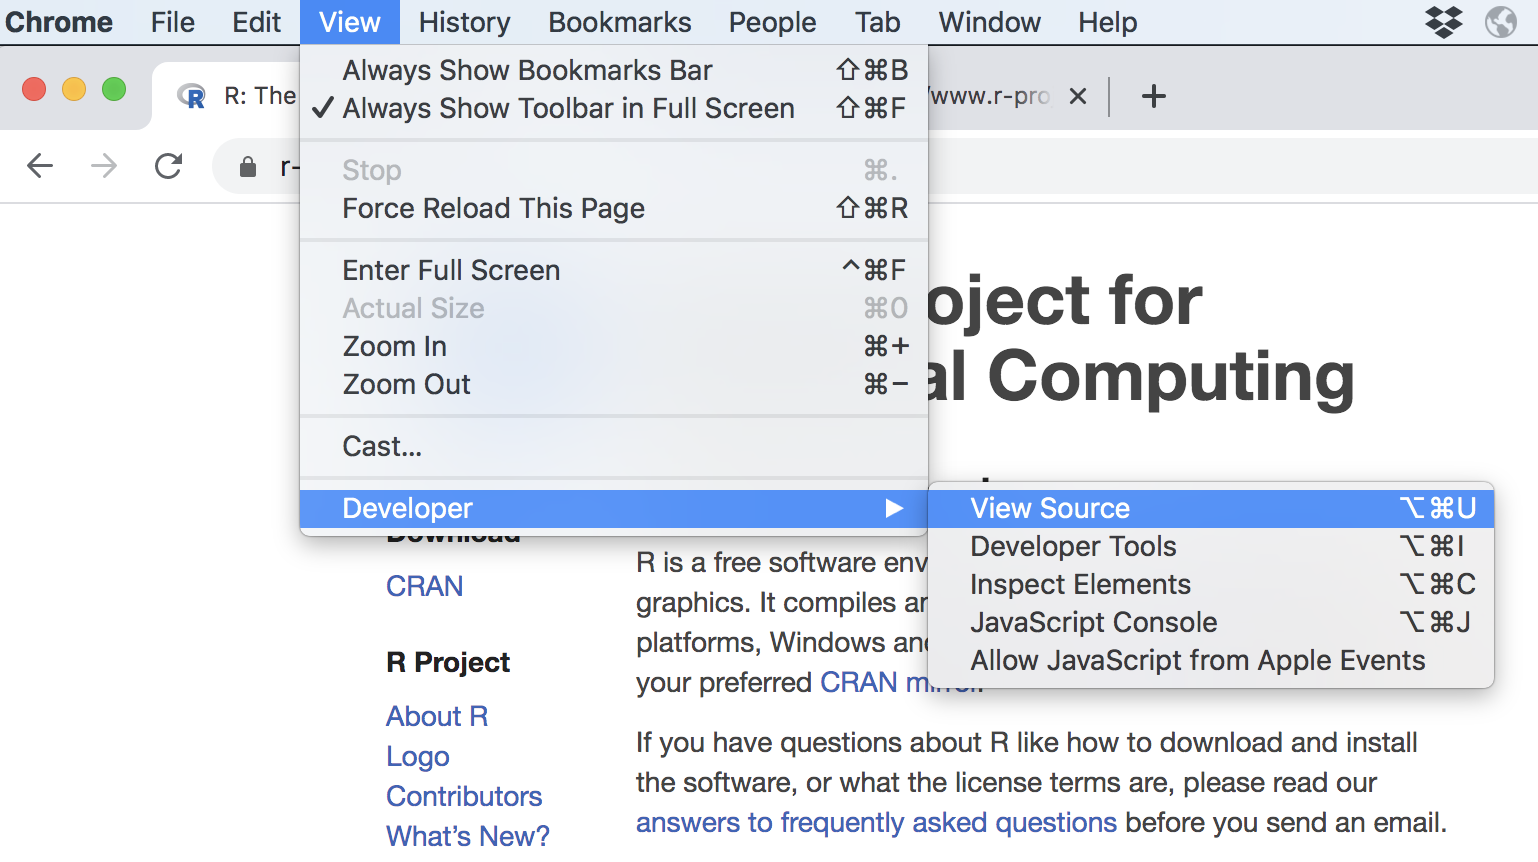
\includegraphics[width=0.75\linewidth]{images/html/r-webpage3} 

}

\caption{View source code of a webpage in Chrome}\label{fig:unnamed-chunk-74}
\end{figure}

If we take a look at the source file behind R's homepage, we'll discover the
actual HTML content, depicted in the image below.

\begin{figure}

{\centering 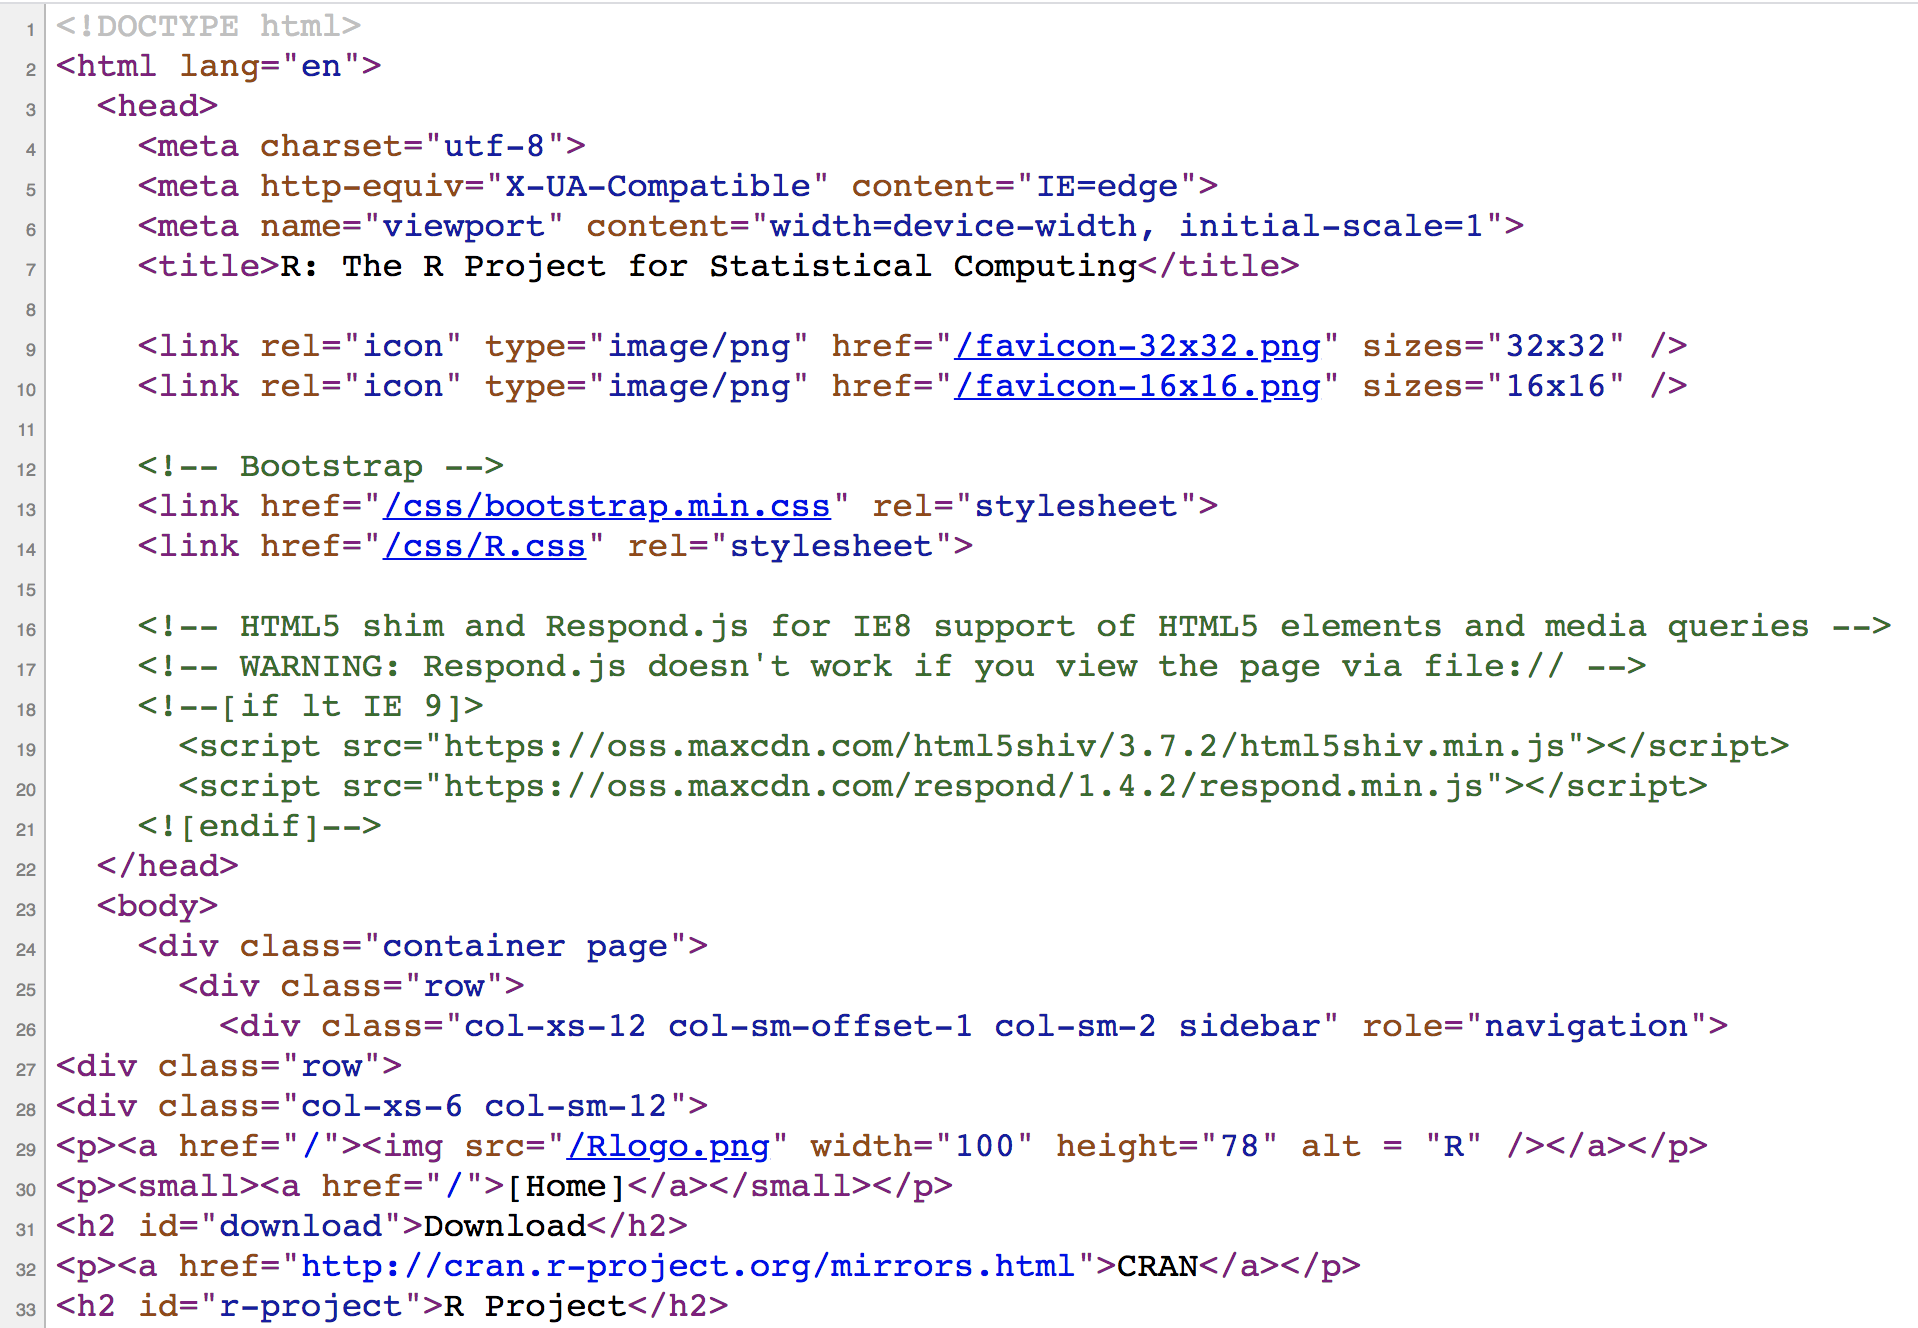
\includegraphics[width=0.75\linewidth]{images/html/r-webpage-source1} 

}

\caption{HTML source code behind R project's home page}\label{fig:unnamed-chunk-75}
\end{figure}

As you can tell, the webpage is cleverly rendered by your browser that knows
exactly how to take care of the content in the source file. If you are not
familiar with HTML, some (if not most) of the text will look like gibberish to
you right now. But it all has a specific structure and meaning.

What you see on the browser is the result of the resources served by the server
where R's website is stored. Technically speaking, the resources should include
an \texttt{index.html}file, plus other files (stylesheet files, and image files)

\begin{figure}

{\centering 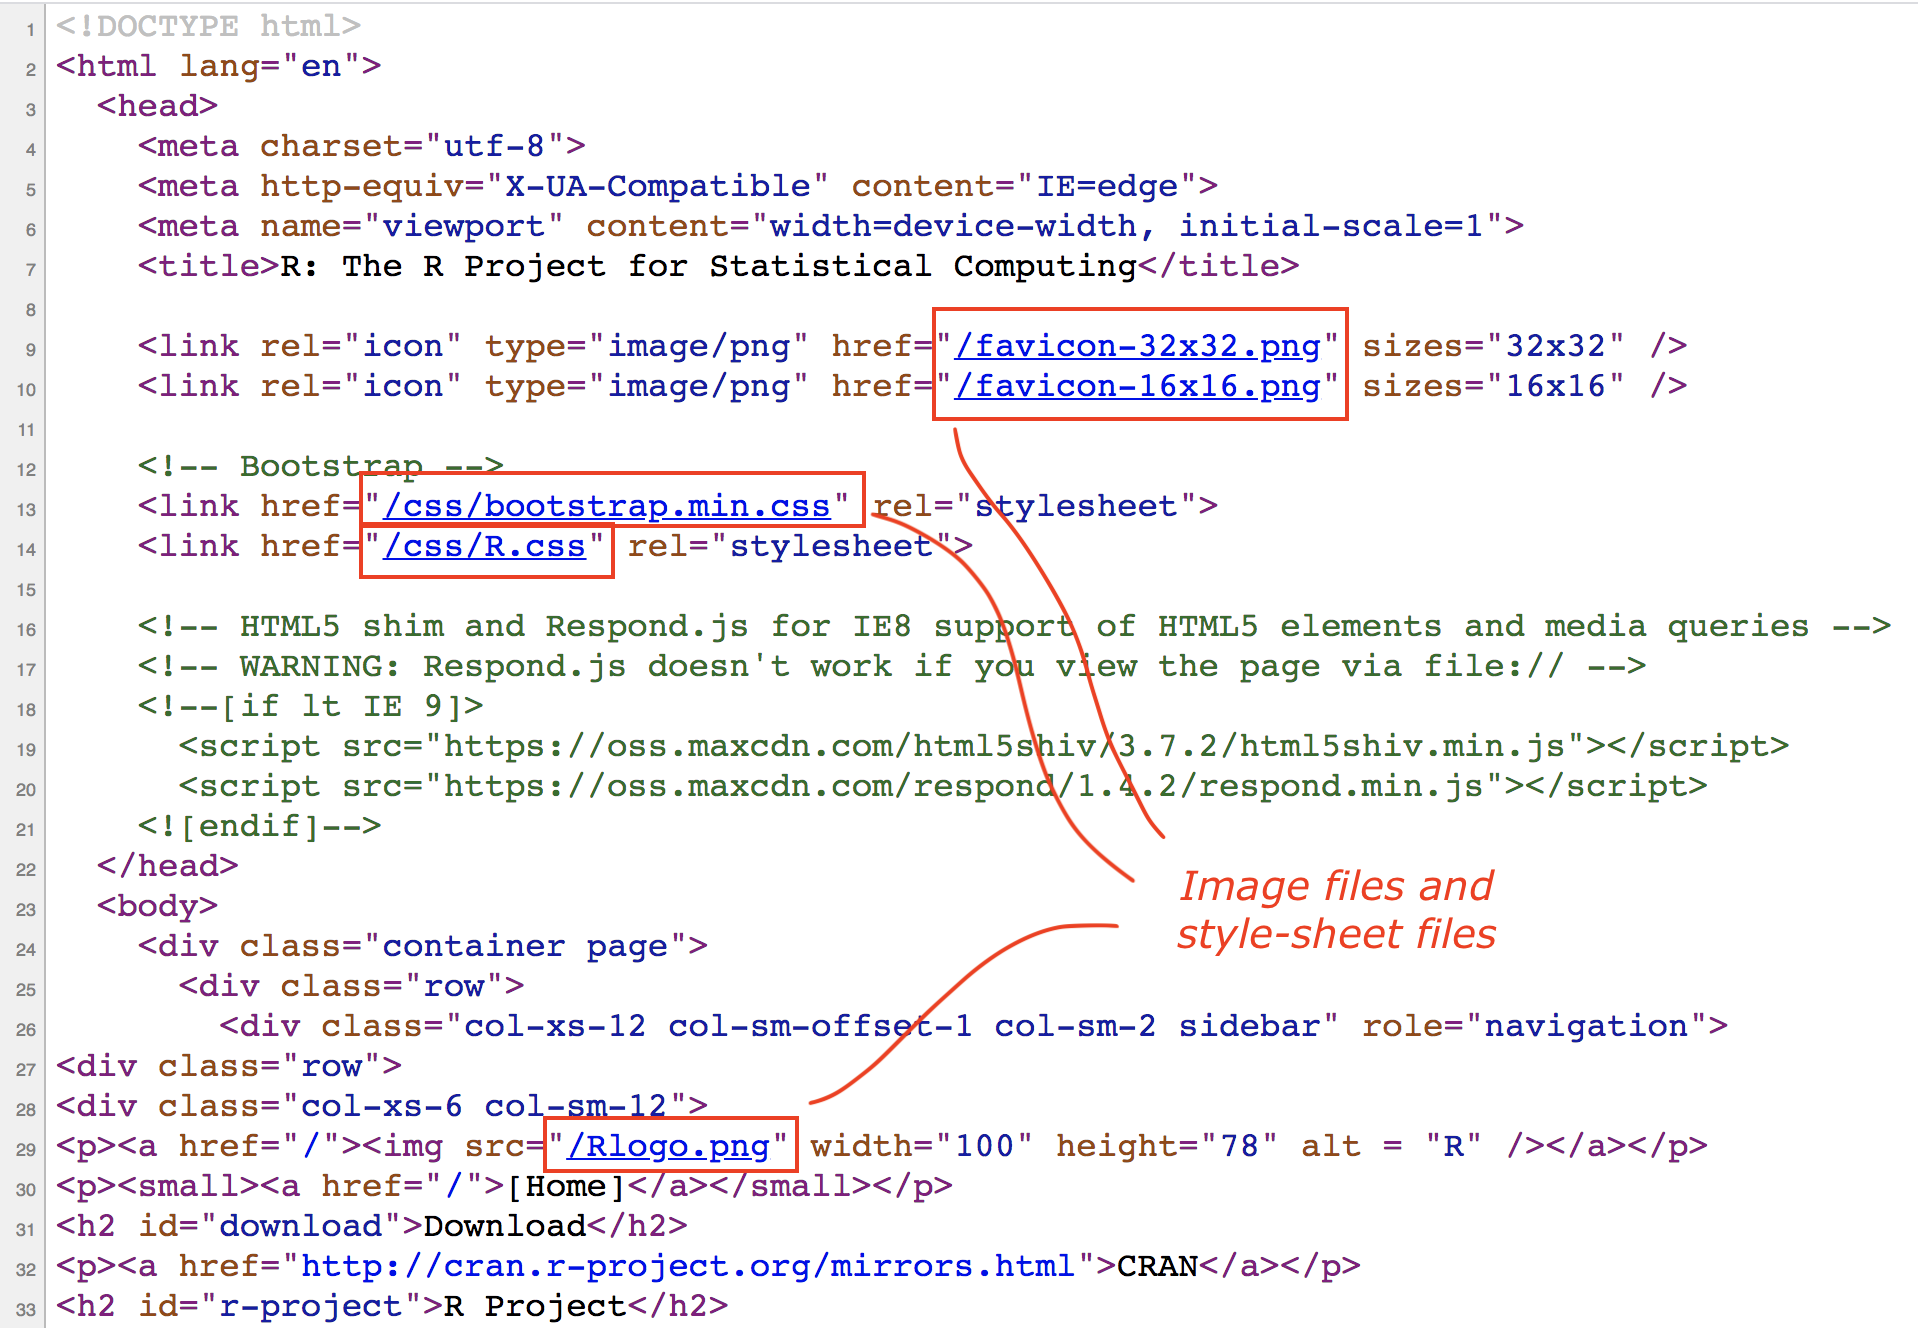
\includegraphics[width=0.7\linewidth]{images/html/r-webpage-source2} 

}

\caption{Other resources being linked in the home page}\label{fig:unnamed-chunk-76}
\end{figure}

In particular, the following resources (different types of files) can be
identified:

\begin{itemize}
\tightlist
\item
  \texttt{index.html}
\item
  \texttt{favicon-33x32.png}
\item
  \texttt{favicon-16x16.png}
\item
  \texttt{bootstrap.min.css}
\item
  \texttt{R.css}
\item
  \texttt{Rlogo.png}
\end{itemize}

\hypertarget{html-document-structure}{%
\subsection{HTML document structure}\label{html-document-structure}}

Let's study the structure of a basic HTML document. Below is a diagram with a
simplified content of R's webpage.

\begin{figure}

{\centering 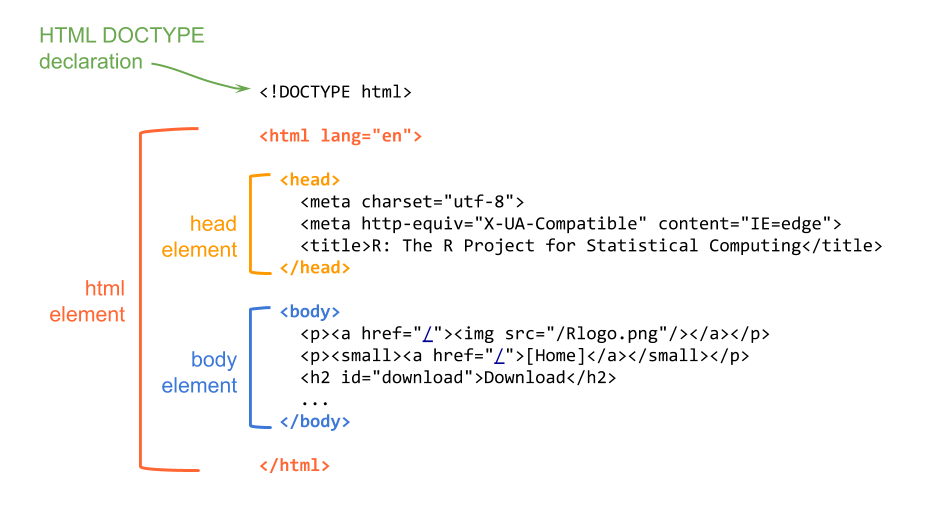
\includegraphics[width=0.8\linewidth]{images/html/r-webpage-source3} 

}

\caption{HTML document structure}\label{fig:unnamed-chunk-77}
\end{figure}

The first line of text is the \emph{document type declaration}, which identifies
this document as an HTML5 document.
Then we have the \textbf{html} element which is the root element of the document,
and it contains all the other elements.

Within the \textbf{html} element, we find two elements: the \textbf{head} and the
\textbf{body}. The \emph{head} element contains descriptive information such as the
title, style sheets, scripts, and other meta information. The mandatory element
inside the head is the \textbf{title}.

The \textbf{body} element contains everything that is displayed in the browser.

\hypertarget{html-syntax}{%
\subsection{HTML Syntax}\label{html-syntax}}

You don't need to memorize all possible HTML elements (or tags), but it's
important that you learn about their syntax and structure. So let's describe
the anatomy of html elements.

Here's an example with a \texttt{\textless{}p\textgreater{}} element which is the \textbf{paragraph} element.
An HTML tag has an opening tag consisting of the tag name surrounded by angle
brackets, that is, the \texttt{\textless{}p\textgreater{}} characters.

Usually, you put tags around some \emph{content} text. At the end of the tag there
is the closing tag, in this case \texttt{\textless{}/p\textgreater{}}. You know it's a closing tag because
it comes after the content, and it has a slash \texttt{/} before the \texttt{p} name. All
closing tags have a slash in them.

\begin{figure}

{\centering 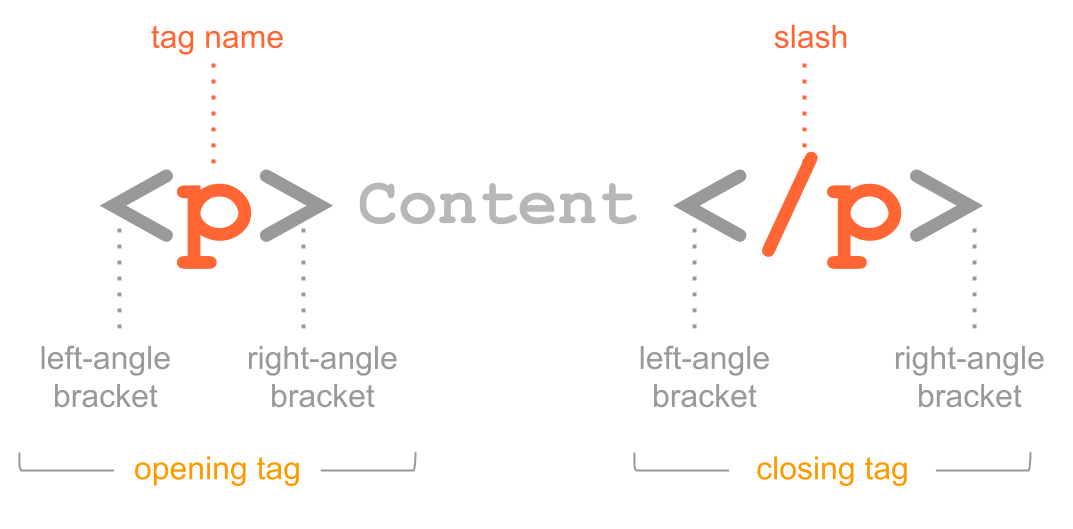
\includegraphics[width=0.7\linewidth]{images/html/html-syntax1} 

}

\caption{Anatomy of html elements}\label{fig:unnamed-chunk-78}
\end{figure}

Not all tags come in the form of a pair of matching tags (an opening and a
closing tag). There are some tags that don't have a closing tag. Perhaps the
most common tag of this type is the \texttt{\textless{}img\textgreater{}} tag used for images. One example
is the \texttt{\textless{}img\textgreater{}} tag for the R logo file in the homepage of R project:

\begin{verbatim}
<img src="/Rlogo.png"/>
\end{verbatim}

As you can tell, the \texttt{\textless{}img\textgreater{}} tag does not have a closing tag; you can say
that itself closes with a slash and the right angle bracket \texttt{/\textgreater{}}.

Some elements have \textbf{attributes} which allows you to specify additional
information about an element. Attributes are declared inside the opening
tag using special keywords. We assign values to attributes with the equals
sign, and we specify the values inside quotations.

\begin{figure}

{\centering 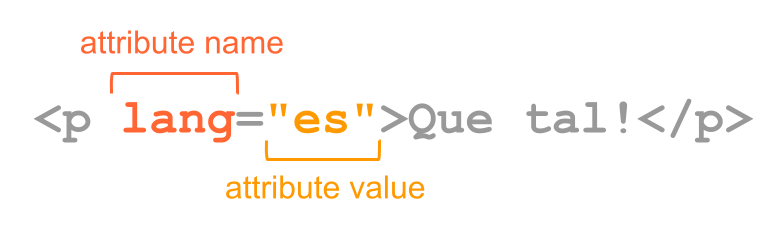
\includegraphics[width=0.7\linewidth]{images/html/html-syntax2} 

}

\caption{Attributes and values in html tags}\label{fig:unnamed-chunk-79}
\end{figure}

In the example above, a paragraph tag contains an attribute \texttt{lang} for
\emph{language} with a value of \texttt{es} for \emph{español} or spanish.

Notice also that the previous \texttt{\textless{}img\textgreater{}} element has an attribute \texttt{src}
to indicate the source filename of the picture, in this case, \texttt{"/Rlogo.png"}.

\hypertarget{what-the-browser-does}{%
\subsection{What the browser does}\label{what-the-browser-does}}

The browser (e.g.~Chrome, Safari, Firefox) reads the HTML, interprets all the
tags, and renders the content accordingly. Recall that tags tell browser about
the structure and meaning of the text. The browser identifies what parts are
headings (e.g.~\texttt{\textless{}h1\textgreater{}}, \texttt{\textless{}h2\textgreater{}}), what parts are paragraphs (e.g.~\texttt{\textless{}p\textgreater{}}),
what parts are lists (e.g.~\texttt{\textless{}ol\textgreater{}}, \texttt{\textless{}ul\textgreater{}}), what text needs to be emphasized,
and so on.

The HTML syntax tells the browser about the structure of a document: where
the headings are, where the paragraphs are, what text is part of a list, and
so on. How do browsers know this? Well, they have built-in default rules
for how to render HTML elements. In addition to the default settings, HTML
elements can be formatted in endless ways using what is called Cascade
Style Sheets or CSS for short, that determine font types, colors, sizes, and
many other visual aspects of a page.

\hypertarget{web-scraping}{%
\subsection{Web Scraping}\label{web-scraping}}

Many websites are secured by an SSL/TSL certificate, which you can identify by
looking at the URL containing \texttt{https} (Hyper Text Transfer Protocol Secure).
SSL stands for \textbf{Secure Sockets Layer}. This is a technology that
keeps an internet connection secure and safeguards sensitive data that is being
sent between a client and a server (for example, when you use your browser
to shop in amazon) or server to server (for example, an application with
payroll information). The SSL technology is currently deprecated and has been
replaced entirely by TLS which stands for \textbf{Transport Layer Security}. Simply
put, TSL also ensures data privacy the same way that SSL does. Since SSL is
actually no longer used, this is the correct term that people should start using.

HTTPS is a secure extension of HTTP. When a website uses HTTPS it means that
the website is secured by an SSL/TLS certificate. Consequently, websites that
install and configure an SSL/TLS certificate can use the HTTPS protocol to
establish a secure connection with the server.
\textbf{Quote}: ``The details of the certificate, including the issuing
authority and the corporate name of the website owner, can be viewed by
clicking on the lock symbol on the browser bar.''

Wikipedia uses HTTPS. For instance, if we visit the entry for men's long jump
world record progression, the url is

\url{https://en.wikipedia.org/wiki/Men\%27s_long_jump_world_record_progression}

If we try to use functions like \texttt{readHTMLTable} from \texttt{"XML"} package, it will
fail

\begin{Shaded}
\begin{Highlighting}[]
\NormalTok{wiki }\OtherTok{\textless{}{-}} \StringTok{\textquotesingle{}https://en.wikipedia.org/wiki/Men\%27s\_long\_jump\_world\_record\_progression\textquotesingle{}}

\CommentTok{\# this fails}
\NormalTok{tbls }\OtherTok{\textless{}{-}} \FunctionTok{readHTMLTable}\NormalTok{(wiki)}
\end{Highlighting}
\end{Shaded}

One option to read the html tables and extract them as R data frames, is to
first download the html file to your computer, and then use \texttt{readHTMLTable()}
to scrape the tables:

\begin{Shaded}
\begin{Highlighting}[]
\CommentTok{\# desired url}
\NormalTok{wiki }\OtherTok{\textless{}{-}} \StringTok{\textquotesingle{}https://en.wikipedia.org/wiki/Men\%27s\_long\_jump\_world\_record\_progression\textquotesingle{}}

\CommentTok{\# destination file}
\NormalTok{jump\_html }\OtherTok{\textless{}{-}} \StringTok{\textquotesingle{}men{-}long{-}jump{-}records.html\textquotesingle{}}

\CommentTok{\# download file to your working directory}
\FunctionTok{download.file}\NormalTok{(wiki, jump\_html)}

\NormalTok{tbls }\OtherTok{\textless{}{-}} \FunctionTok{readHTMLTable}\NormalTok{(jump\_html)}
\end{Highlighting}
\end{Shaded}

We recommend using this option when:

\begin{itemize}
\tightlist
\item
  the data fits in your computer, in this way you also have the \emph{raw data}
\item
  you need to experiment and get to know the content, in order to decide
  which elements you will extract, which functions to use, what kind of processing
  operations or transformations you need to apply, etc.
\item
  also, downloading an HTML document save you from making innecessary requests
  that could get in trouble, and potentially be blocked by a server because you
  are overloading them with multiple requests.
\end{itemize}

\hypertarget{part-json}{%
\part{JSON}\label{part-json}}

\hypertarget{json}{%
\chapter{JSON Data}\label{json}}

The goal of this chapter is to provide an introduction for handling JSON data
in R.

We'll cover the following topics:

\begin{itemize}
\tightlist
\item
  JSON Basics
\item
  R packages for JSON data
\item
  Reading JSON data from the Web
\end{itemize}

\hypertarget{json-basics}{%
\section{JSON Basics}\label{json-basics}}

JSON stands for \textbf{JavaScript Object Notation} and it is a format for
representing data. More formally, we can say that it is a text-based way to
store and transmit structured data. By using a simple syntax, you can easily
store anything from a single number to strings, JSON-arrays, and JSON-objects
using nothing but a string of plain text. As you will see, you can also nest
arrays and objects, allowing you to create complex data structures.

\hypertarget{what-is-json}{%
\section{What is JSON?}\label{what-is-json}}

Let's first talk about what JSON is and why it is important.

JSON is a data representation format very similar to XML. It's used widely
across the internet for almost every single API that you will access as well as
for \emph{config} files and things such as games and text editors. Its popularity
is based on a handful of attractive aspects:

\begin{itemize}
\item
  It's extremely lightweight and compact to send back and forth due to the small
  size file;
\item
  It's easy for both computers and people to read-and-write, compared to
  something like XML, since it's much cleaner and there's not as many opening and
  closing tags;
\item
  It maps very easily onto the data structures used by most programming
  languages (numbers, strings, booleans, nulls, arrays and associative arrays);
\item
  It also integrates very nicely with
  javascript
  since JSON is just a superset of
  javascript
  which means anything you write in JSON is valid javascript, which is a language
  used all throughout the web for front-end or back-end of applications.
\item
  Also, every single major language has some form of library or packages with
  built-in functionality to parse JSON strings into objects or classes in that
  language which makes working with JSON data extremely easy inside of a
  programming language.
\end{itemize}

Why should we care about JSON? When working with data from the Web, we'll
inevitably find some JSON data because it is commonly used in web applications
to send data from the server to the browser. As a matter of fact, in your data
science career you will be using JSON quite often, whether it is consuming an
API, creating an API, or creating \emph{config} files for you or other people to use
for your application.

\hypertarget{understanding-json-syntax}{%
\section{Understanding JSON Syntax}\label{understanding-json-syntax}}

Let's now talk about the syntax used to store and organize data in JSON.

\hypertarget{data-types}{%
\subsection{Data Types}\label{data-types}}

The first thing to talk about is the \textbf{data types} or \textbf{values} that JSON can
represent. As we know, JSON is a data representation format, so we need to be
able to represent certain data types within it. JSON supports the following types:

\begin{itemize}
\item
  \texttt{string} (in double quotes)
\item
  \texttt{number} (in any format whether they're decimal numbers, integers, negative
  numbers, even numbers in scientific notation)
\item
  \texttt{true} and \texttt{false} (booleans)
\item
  \texttt{null}
\end{itemize}

\hypertarget{arrays}{%
\subsection{Arrays}\label{arrays}}

JSON also supports \textbf{arrays} (in JSON Sense) which are sets of data types
defined within brackets, and contains a comma-separated list of values.
For example \texttt{{[}1,\ 3,\ 3{]}} or \texttt{{[}"computing",\ "with",\ "data"{]}},
which can be a set of any of the data types listed above.

We typically use arrays when we have a set of unnamed values, this is why some
people refer to them as \textbf{ordered unnamed arrays}. The closest R object to a
JSON array would be a vector:

\begin{itemize}
\item
  JSON: \texttt{{[}1,\ 2,\ 3,\ ...\ {]}}; -vs- R: \texttt{c(1,\ 2,\ 3,\ ...)}
\item
  JSON: \texttt{{[}true,\ true,\ false,\ ...\ {]}}; -vs- R: \texttt{c(TRUE,\ TRUE,\ FALSE,\ ...)}
\end{itemize}

\hypertarget{objects}{%
\subsection{Objects}\label{objects}}

Another type of data container is the so-called JSON \textbf{object}, which is the
most complex but also the most used type of object within JSON, and it allows
you to represent values that are key-value pairs:

\texttt{\{"key":\ "value"\}}

You use curly braces to define a JSON-object, and inside the braces you put
key-value pairs. The key must be surrounded by double quotes, followed by a
colon, followed by the value. The value can be a single data type, but it
can also be a JSON-array (which in turn can contain a JSON-object). Because
you have the association of a \emph{key} with its \emph{value}, these JSON structures
are also referred to as associative arrays.

For example, say the key is \texttt{"year"} and the value \texttt{2000}, then a simple JSON
object will look like this:

\texttt{\{"year":\ 2000\}}

Another example can be a key \texttt{"name"} and a value \texttt{"Jessica"}:

\texttt{\{"name":\ "Jessica"\}}

If you have multiple key-value pairs, you separate each of them with a comma:

\begin{verbatim}
{
  "name1": "Nicole",
  "name2": "Pleuni",
  "name3": "Rori"
}
\end{verbatim}

A more complex object might look like the following example. In this case we
have JSON-object that contains three key-value pairs. Each of the keys is a
\texttt{"person"} and the associated pair corresponds to an array which in turn
contains a JSON-object with two key-value pairs: the \emph{first name}, and the
\emph{last name}:

\begin{verbatim}
{
  "person1": [
    {
      "first": "Nicole",
      "last": "Adelstein"
    }
  ],
  "person2": [
    {
      "first": "Pleuni",
      "last": "Pennings"
    }
  ],
  "person3": [
    {
      "first": "Rori",
      "last": "Rohlfs"
    }
  ]
}
\end{verbatim}

Because the data inside a JSON object is formed of key-value pairs, you could
think of them as \textbf{named arrays}.

What do JSON-objects correspond to in R? Well, there's not really a unique
correspondence between a JSON-object and its equivalent in structure R. For
instance, let's bring back one of the JSON-objects previously discussed:

\begin{verbatim}
{
  "name1": "Nicole",
  "name2": "Pleuni",
  "name3": "Rori"
}
\end{verbatim}

We could use a named R vector to store the same data:

\begin{Shaded}
\begin{Highlighting}[]
\CommentTok{\# named vector in R}
\FunctionTok{c}\NormalTok{(}\StringTok{"name1"} \OtherTok{=} \StringTok{"Nicole"}\NormalTok{, }\StringTok{"name2"} \OtherTok{=} \StringTok{"Pleuni"}\NormalTok{, }\StringTok{"name3"} \OtherTok{=} \StringTok{"Rori"}\NormalTok{)}
\end{Highlighting}
\end{Shaded}

But we could also use an R list:

\begin{Shaded}
\begin{Highlighting}[]
\CommentTok{\# named list in R}
\FunctionTok{list}\NormalTok{(}\StringTok{"name1"} \OtherTok{=} \StringTok{"Nicole"}\NormalTok{, }\StringTok{"name2"} \OtherTok{=} \StringTok{"Pleuni"}\NormalTok{, }\StringTok{"name3"} \OtherTok{=} \StringTok{"Rori"}\NormalTok{)}
\end{Highlighting}
\end{Shaded}

Keep in mind that JSON-objects can be more complex than this basic example.
Because JSON objects can contain any other type of JSON data structure in them,
the similar container in R to a JSON-object is a \texttt{list}.

\hypertarget{examples-of-json-data-containers}{%
\subsection{Examples of JSON Data Containers}\label{examples-of-json-data-containers}}

Here's a series of examples involving combinations of JSON arrays and objects.

JSON containers can be nested. Here's one example:

\begin{verbatim}
{
    "name": ["X", "Y", "Z"],
    "grams": [300, 200, 500], 
    "qty": [4, 5, null],
    "new": [true, false, true]
}
\end{verbatim}

Here's another example of nested containers:

\begin{verbatim}
[
    { "name": "X", 
      "grams": 300,
      "qty": 4,
      "new": true },
    { "name": "Y",
      "grams": 200,
      "qty": 5,
      "new": false },
    { "name": "Z",
      "grams": 500, 
      "qty": null,
      "new": true}
]
\end{verbatim}

\hypertarget{data-table-toy-example}{%
\subsection{Data Table Toy Example}\label{data-table-toy-example}}

Let's consider a less basic example with some tabular data set:

\begin{longtable}[]{@{}lllll@{}}
\toprule\noalign{}
Name & Gender & Homeland & Born & Jedi \\
\midrule\noalign{}
\endhead
\bottomrule\noalign{}
\endlastfoot
Anakin & male & Tatooine & 41.9BBY & yes \\
Amidala & female & Naboo & 46BBY & no \\
Luke & male & Tatooine & 19BBY & yes \\
Leia & female & Alderaan & 19BBY & no \\
Obi-Wan & male & Stewjon & 57BBY & yes \\
Han & male & Corellia & 29BBY & no \\
Palpatine & male & Naboo & 82BBY & no \\
R2-D2 & unknown & Naboo & 33BBY & no \\
\end{longtable}

How can we store this tabular data in JSON format? There are several ways to
represent this data in JSON format. One option could be a JSON-array containing
JSON-objects. Each JSON-object represents an individual:

\begin{verbatim}
    [
        {
         "Name": "Anakin",
         "Gender": "male", 
         "Homeworld": "Tatooine",
         "Born": "41.9BBY",
         "Jedi": "yes"
        },
        {
         "Name": "Amidala",
         "Gender": "female", 
         "Homeworld": "Naboo",
         "Born": 46BBY",
         "Jedi": "no"
        },
        ...
        {
         "Name": "R2-D2",
         "Gender": "unknown",
         "Homeworld": "Naboo",
         "Born": "33BBY",
         "Jedi": "no"
        }
    ]
\end{verbatim}

Another way to represent the data in the table above is by using an object
containing key-value pairs in which the \emph{keys} are the names of the columns,
and the \emph{pairs} are arrays (the data values in each column).

\begin{verbatim}
{
  "Name": [ "Anakin", "Amidala", "Luke", ... , "R2-D2" ],
  "Gender": [ "male", "female", "male", ... , "unknown" ],
  "Homeworld": [ "Tatooine", "Naboo", "Tatooine", ... , "Naboo" ],
  "Born": [ "41.9BBY", "46BBY", "19BBY", ... , "33BBY" ],
  "Jedi": [ "yes", "no", "yes", ... , "no" ] 
}
\end{verbatim}

\hypertarget{jsonlite}{%
\chapter{JSON R packages}\label{jsonlite}}

R has 3 packages for working with JSON data

\begin{itemize}
\item
  \texttt{"RJSONIO"} by Duncan Temple Lang
\item
  \texttt{"rjson"} by Alex Couture-Beil
\item
  \texttt{"jsonlite"} by Jeroen Ooms, Duncan Temple Lang, Jonathan Wallace
\end{itemize}

All packages provide 2 main functions, \texttt{toJSON()} and \texttt{fromJSON()}, that allow
conversion \textbf{to} and \textbf{from} data in JSON format, respectively.
We'll focus on the functions from \texttt{"jsonlite"}.

For illustration purposes, let us consider the package \texttt{"jsonlite"}.

There are 2 primary functions in \texttt{"jsonlite"}:

\begin{itemize}
\item
  \texttt{toJSON()} converts an R object to a string in JSON
\item
  \texttt{fromJSON()} converts JSON content to R objects
\end{itemize}

\hypertarget{function-tojson}{%
\section{\texorpdfstring{Function \texttt{toJSON()}}{Function toJSON()}}\label{function-tojson}}

The function \texttt{jsonlite::toJSON()} converts an R object to a string in JSON.

\hypertarget{example-single-number-to-json-array}{%
\subsubsection*{Example: single number to JSON-array}\label{example-single-number-to-json-array}}
\addcontentsline{toc}{subsubsection}{Example: single number to JSON-array}

Let's begin with a super simple example by passing a single data value to the
function \texttt{toJSON()}:

\begin{Shaded}
\begin{Highlighting}[]
\FunctionTok{toJSON}\NormalTok{(pi, }\AttributeTok{digits =} \DecValTok{4}\NormalTok{)}
\CommentTok{\#\textgreater{} [3.1416]}
\end{Highlighting}
\end{Shaded}

\hypertarget{example-vectors-to-json-arrays}{%
\subsubsection*{Example: vectors to JSON-arrays}\label{example-vectors-to-json-arrays}}
\addcontentsline{toc}{subsubsection}{Example: vectors to JSON-arrays}

Consider the following vectors

\begin{Shaded}
\begin{Highlighting}[]
\NormalTok{num }\OtherTok{\textless{}{-}} \FunctionTok{c}\NormalTok{(}\DecValTok{1}\NormalTok{, }\DecValTok{2}\NormalTok{, }\DecValTok{3}\NormalTok{, }\DecValTok{4}\NormalTok{, }\DecValTok{5}\NormalTok{)}
\NormalTok{lts }\OtherTok{\textless{}{-}} \FunctionTok{c}\NormalTok{(}\StringTok{\textquotesingle{}a\textquotesingle{}}\NormalTok{, }\StringTok{\textquotesingle{}b\textquotesingle{}}\NormalTok{, }\StringTok{\textquotesingle{}c\textquotesingle{}}\NormalTok{, }\StringTok{\textquotesingle{}d\textquotesingle{}}\NormalTok{, }\StringTok{\textquotesingle{}e\textquotesingle{}}\NormalTok{)}
\end{Highlighting}
\end{Shaded}

Applying \texttt{toJSON()} to the vectors \texttt{num} and \texttt{lts} produces JSON arrays:

\begin{Shaded}
\begin{Highlighting}[]
\FunctionTok{toJSON}\NormalTok{(num)}
\CommentTok{\#\textgreater{} [1,2,3,4,5]}

\FunctionTok{toJSON}\NormalTok{(lts)}
\CommentTok{\#\textgreater{} ["a","b","c","d","e"]}
\end{Highlighting}
\end{Shaded}

The argument \texttt{pretty\ =\ TRUE} allows you to obtain a JSON string with added
indentation whitespace:

\begin{Shaded}
\begin{Highlighting}[]
\FunctionTok{toJSON}\NormalTok{(num, }\AttributeTok{pretty =} \ConstantTok{TRUE}\NormalTok{)}
\CommentTok{\#\textgreater{} [1, 2, 3, 4, 5]}

\FunctionTok{toJSON}\NormalTok{(lts, }\AttributeTok{pretty =} \ConstantTok{TRUE}\NormalTok{)}
\CommentTok{\#\textgreater{} ["a", "b", "c", "d", "e"]}
\end{Highlighting}
\end{Shaded}

What about an R vector with named elements? For example, here's a vector \texttt{vec}

\begin{Shaded}
\begin{Highlighting}[]
\NormalTok{vec }\OtherTok{\textless{}{-}}\NormalTok{ num}
\FunctionTok{names}\NormalTok{(vec) }\OtherTok{\textless{}{-}}\NormalTok{ lts}
\NormalTok{vec}
\CommentTok{\#\textgreater{} a b c d e }
\CommentTok{\#\textgreater{} 1 2 3 4 5}
\end{Highlighting}
\end{Shaded}

Converting \texttt{vec} to JSON, we get:

\begin{Shaded}
\begin{Highlighting}[]
\FunctionTok{toJSON}\NormalTok{(vec)}
\CommentTok{\#\textgreater{} [1,2,3,4,5]}
\end{Highlighting}
\end{Shaded}

As you can tell, the names of the elements in \texttt{vec} are lost in translation.

\hypertarget{example-matrix-to-json-array}{%
\subsubsection*{Example: matrix to JSON-array}\label{example-matrix-to-json-array}}
\addcontentsline{toc}{subsubsection}{Example: matrix to JSON-array}

Here's another example from an matrix to a JSON array:

\begin{Shaded}
\begin{Highlighting}[]
\NormalTok{mat }\OtherTok{\textless{}{-}} \FunctionTok{matrix}\NormalTok{(}\DecValTok{9}\SpecialCharTok{:}\DecValTok{1}\NormalTok{, }\AttributeTok{nrow =} \DecValTok{3}\NormalTok{, }\AttributeTok{ncol =} \DecValTok{3}\NormalTok{)}
\NormalTok{mat}
\CommentTok{\#\textgreater{}      [,1] [,2] [,3]}
\CommentTok{\#\textgreater{} [1,]    9    6    3}
\CommentTok{\#\textgreater{} [2,]    8    5    2}
\CommentTok{\#\textgreater{} [3,]    7    4    1}
\end{Highlighting}
\end{Shaded}

\texttt{toJSON()} converts an R matrix into a JSON-array

\begin{Shaded}
\begin{Highlighting}[]
\FunctionTok{toJSON}\NormalTok{(mat)}
\CommentTok{\#\textgreater{} [[9,6,3],[8,5,2],[7,4,1]]}
\end{Highlighting}
\end{Shaded}

Notice that the returned output arranges the values of the matrix row-by-row,
also referred to as \emph{row-major}. This means that when the input is an R matrix,
\texttt{toJSON()} uses its argument \texttt{matrix\ =\ "rowmajor"}.

You can change the arrangement to \emph{column-major} by specifying the argument
\texttt{matrix\ =\ "columnmajor"}:

\begin{Shaded}
\begin{Highlighting}[]
\FunctionTok{toJSON}\NormalTok{(mat, }\AttributeTok{matrix =} \StringTok{"columnmajor"}\NormalTok{)}
\CommentTok{\#\textgreater{} [[9,8,7],[6,5,4],[3,2,1]]}
\end{Highlighting}
\end{Shaded}

\hypertarget{example-data-frame-to-json-object}{%
\subsubsection*{Example: data frame to JSON-object}\label{example-data-frame-to-json-object}}
\addcontentsline{toc}{subsubsection}{Example: data frame to JSON-object}

We can also use \texttt{toJSON()} on data frames. Here's an example of an assembled
data frame \texttt{swdf} which will be converted to a JSON-object:

\begin{Shaded}
\begin{Highlighting}[]
\CommentTok{\# toy data}
\NormalTok{sw\_data }\OtherTok{\textless{}{-}} \FunctionTok{rbind}\NormalTok{(}
  \FunctionTok{c}\NormalTok{(}\StringTok{"Anakin"}\NormalTok{, }\StringTok{"male"}\NormalTok{, }\StringTok{"Tatooine"}\NormalTok{, }\StringTok{"41.9BBY"}\NormalTok{,  }\StringTok{"yes"}\NormalTok{),  }
  \FunctionTok{c}\NormalTok{(}\StringTok{"Amidala"}\NormalTok{, }\StringTok{"female"}\NormalTok{, }\StringTok{"Naboo"}\NormalTok{, }\StringTok{"46BBY"}\NormalTok{, }\StringTok{"no"}\NormalTok{),}
  \FunctionTok{c}\NormalTok{(}\StringTok{"Luke"}\NormalTok{, }\StringTok{"male"}\NormalTok{, }\StringTok{"Tatooine"}\NormalTok{, }\StringTok{"19BBY"}\NormalTok{, }\StringTok{"yes"}\NormalTok{),}
  \FunctionTok{c}\NormalTok{(}\StringTok{"Leia"}\NormalTok{, }\StringTok{"female"}\NormalTok{, }\StringTok{"Alderaan"}\NormalTok{, }\StringTok{"19BBY"}\NormalTok{, }\StringTok{"no"}\NormalTok{)}
\NormalTok{)}

\CommentTok{\# convert to data.frame and add column names}
\NormalTok{swdf }\OtherTok{\textless{}{-}} \FunctionTok{data.frame}\NormalTok{(sw\_data, }\AttributeTok{stringsAsFactors =} \ConstantTok{FALSE}\NormalTok{)}
\FunctionTok{names}\NormalTok{(swdf) }\OtherTok{\textless{}{-}} \FunctionTok{c}\NormalTok{(}\StringTok{"Name"}\NormalTok{, }\StringTok{"Gender"}\NormalTok{, }\StringTok{"Homeworld"}\NormalTok{, }\StringTok{"Born"}\NormalTok{, }\StringTok{"Jedi"}\NormalTok{)}
\NormalTok{swdf}
\CommentTok{\#\textgreater{}      Name Gender Homeworld    Born Jedi}
\CommentTok{\#\textgreater{} 1  Anakin   male  Tatooine 41.9BBY  yes}
\CommentTok{\#\textgreater{} 2 Amidala female     Naboo   46BBY   no}
\CommentTok{\#\textgreater{} 3    Luke   male  Tatooine   19BBY  yes}
\CommentTok{\#\textgreater{} 4    Leia female  Alderaan   19BBY   no}
\end{Highlighting}
\end{Shaded}

The default output when you pass a data frame to \texttt{jsonlite::toJSON()} is

\begin{Shaded}
\begin{Highlighting}[]
\CommentTok{\# convert R data.frame to JSON}
\NormalTok{sw\_json }\OtherTok{=} \FunctionTok{toJSON}\NormalTok{(swdf)}
\NormalTok{sw\_json}
\CommentTok{\#\textgreater{} [\{"Name":"Anakin","Gender":"male","Homeworld":"Tatooine","Born":"41.9BBY","Jedi":"yes"\},\{"Name":"Amidala","Gender":"female","Homeworld":"Naboo","Born":"46BBY","Jedi":"no"\},\{"Name":"Luke","Gender":"male","Homeworld":"Tatooine","Born":"19BBY","Jedi":"yes"\},\{"Name":"Leia","Gender":"female","Homeworld":"Alderaan","Born":"19BBY","Jedi":"no"\}]}
\end{Highlighting}
\end{Shaded}

The argument \texttt{dataframe} gives you more control on the output. This argument
has three options:

\begin{itemize}
\tightlist
\item
  \texttt{"rows"}: each row is converted to a JSON-object with \emph{key-value} pairs
  formed by \texttt{"column\_name":\ "row\_value"};
\end{itemize}

\begin{Shaded}
\begin{Highlighting}[]
\FunctionTok{toJSON}\NormalTok{(swdf, }\AttributeTok{dataframe =} \StringTok{"rows"}\NormalTok{)}
\CommentTok{\#\textgreater{} [\{"Name":"Anakin","Gender":"male","Homeworld":"Tatooine","Born":"41.9BBY","Jedi":"yes"\},\{"Name":"Amidala","Gender":"female","Homeworld":"Naboo","Born":"46BBY","Jedi":"no"\},\{"Name":"Luke","Gender":"male","Homeworld":"Tatooine","Born":"19BBY","Jedi":"yes"\},\{"Name":"Leia","Gender":"female","Homeworld":"Alderaan","Born":"19BBY","Jedi":"no"\}]}
\end{Highlighting}
\end{Shaded}

\begin{itemize}
\tightlist
\item
  \texttt{"columns"}: each column is converted into a JSON-object with a single \emph{key}
  for each column, and \emph{values} stored as arrays;
\end{itemize}

\begin{Shaded}
\begin{Highlighting}[]
\FunctionTok{toJSON}\NormalTok{(swdf, }\AttributeTok{dataframe =} \StringTok{"columns"}\NormalTok{)}
\CommentTok{\#\textgreater{} \{"Name":["Anakin","Amidala","Luke","Leia"],"Gender":["male","female","male","female"],"Homeworld":["Tatooine","Naboo","Tatooine","Alderaan"],"Born":["41.9BBY","46BBY","19BBY","19BBY"],"Jedi":["yes","no","yes","no"]\}}
\end{Highlighting}
\end{Shaded}

\begin{itemize}
\tightlist
\item
  \texttt{"values"}: the values in each column are converted to a JSON-array, and
  the names of the columns are lost.
\end{itemize}

\begin{Shaded}
\begin{Highlighting}[]
\FunctionTok{toJSON}\NormalTok{(swdf, }\AttributeTok{dataframe =} \StringTok{"values"}\NormalTok{)}
\CommentTok{\#\textgreater{} [["Anakin","male","Tatooine","41.9BBY","yes"],["Amidala","female","Naboo","46BBY","no"],["Luke","male","Tatooine","19BBY","yes"],["Leia","female","Alderaan","19BBY","no"]]}
\end{Highlighting}
\end{Shaded}

\hypertarget{function-fromjson}{%
\section{\texorpdfstring{Function \texttt{fromJSON()}}{Function fromJSON()}}\label{function-fromjson}}

In practice, instead of converting R objects to JSON objects, it is more
common to have data in JSON format which needs to be converted into an R object.

The function \texttt{jsonlite::fromJSON()} converts a JSON-object to an R object.

\hypertarget{example-json-array-to-r-vector}{%
\subsubsection*{Example: JSON-array to R vector}\label{example-json-array-to-r-vector}}
\addcontentsline{toc}{subsubsection}{Example: JSON-array to R vector}

\begin{Shaded}
\begin{Highlighting}[]
\NormalTok{json\_array }\OtherTok{\textless{}{-}} \StringTok{\textquotesingle{}["computing", "with", "data"]\textquotesingle{}}

\FunctionTok{fromJSON}\NormalTok{(json\_array)}
\CommentTok{\#\textgreater{} [1] "computing" "with"      "data"}
\end{Highlighting}
\end{Shaded}

\hypertarget{example-json-object-to-r-object}{%
\subsubsection*{Example: JSON-object to R object}\label{example-json-object-to-r-object}}
\addcontentsline{toc}{subsubsection}{Example: JSON-object to R object}

Consider a simple JSON-object, and its conversion to R with
\texttt{jsonlite::fromJSON()}

\begin{Shaded}
\begin{Highlighting}[]
\NormalTok{json\_obj1 }\OtherTok{\textless{}{-}} \StringTok{\textquotesingle{}\{"name": "Jessica"\}\textquotesingle{}}

\FunctionTok{fromJSON}\NormalTok{(json\_obj1)}
\CommentTok{\#\textgreater{} $name}
\CommentTok{\#\textgreater{} [1] "Jessica"}
\end{Highlighting}
\end{Shaded}

Notice that the obtained object is an R list in which the \emph{key} becomes the
name of the list, and the \emph{value} becomes the content of the list's element.

Consider a less simple JSON-object:

\begin{Shaded}
\begin{Highlighting}[]
\NormalTok{json\_obj2 }\OtherTok{\textless{}{-}} \StringTok{\textquotesingle{}\{"name1": "Nicole", "name2": "Pleuni", "name3": "Rori"\}\textquotesingle{}}

\FunctionTok{fromJSON}\NormalTok{(json\_obj2)}
\CommentTok{\#\textgreater{} $name1}
\CommentTok{\#\textgreater{} [1] "Nicole"}
\CommentTok{\#\textgreater{} }
\CommentTok{\#\textgreater{} $name2}
\CommentTok{\#\textgreater{} [1] "Pleuni"}
\CommentTok{\#\textgreater{} }
\CommentTok{\#\textgreater{} $name3}
\CommentTok{\#\textgreater{} [1] "Rori"}
\end{Highlighting}
\end{Shaded}

Another example:

\begin{Shaded}
\begin{Highlighting}[]
\FunctionTok{fromJSON}\NormalTok{(}\StringTok{\textquotesingle{}\{"name": ["X", "Y"], "grams": [30, 20], "qty": [4, null],}
\StringTok{"new": [true, false]\}\textquotesingle{}}\NormalTok{)}
\CommentTok{\#\textgreater{} $name}
\CommentTok{\#\textgreater{} [1] "X" "Y"}
\CommentTok{\#\textgreater{} }
\CommentTok{\#\textgreater{} $grams}
\CommentTok{\#\textgreater{} [1] 30 20}
\CommentTok{\#\textgreater{} }
\CommentTok{\#\textgreater{} $qty}
\CommentTok{\#\textgreater{} [1]  4 NA}
\CommentTok{\#\textgreater{} }
\CommentTok{\#\textgreater{} $new}
\CommentTok{\#\textgreater{} [1]  TRUE FALSE}
\end{Highlighting}
\end{Shaded}

\hypertarget{example-json-object-to-r-object-1}{%
\subsubsection*{Example: JSON-object to R object}\label{example-json-object-to-r-object-1}}
\addcontentsline{toc}{subsubsection}{Example: JSON-object to R object}

Suppose you have a JSON object with the following data:

\begin{verbatim}
{
  "Name": ["Anakin","Amidala","Luke","Leia"],
  "Gender": ["male","female","male","female"],
  "Homeworld": ["Tatooine","Naboo","Tatooine","Alderaan"],
  "Born": ["41.9BBY","46BBY","19BBY","19BBY"],
  "Jedi": ["yes","no","yes","no"]
}
\end{verbatim}

and assume that the above data is stored as a single (continuous) string in
an R character vector \texttt{json\_sw}; applying \texttt{fromJSON()} to this string gives
you the following list:

\begin{Shaded}
\begin{Highlighting}[]
\FunctionTok{fromJSON}\NormalTok{(json\_sw)}
\CommentTok{\#\textgreater{} $Name}
\CommentTok{\#\textgreater{} [1] "Anakin"  "Amidala" "Luke"    "Leia"   }
\CommentTok{\#\textgreater{} }
\CommentTok{\#\textgreater{} $Gender}
\CommentTok{\#\textgreater{} [1] "male"   "female" "male"   "female"}
\CommentTok{\#\textgreater{} }
\CommentTok{\#\textgreater{} $Homeworld}
\CommentTok{\#\textgreater{} [1] "Tatooine" "Naboo"    "Tatooine" "Alderaan"}
\CommentTok{\#\textgreater{} }
\CommentTok{\#\textgreater{} $Born}
\CommentTok{\#\textgreater{} [1] "41.9BBY" "46BBY"   "19BBY"   "19BBY"  }
\CommentTok{\#\textgreater{} }
\CommentTok{\#\textgreater{} $Jedi}
\CommentTok{\#\textgreater{} [1] "yes" "no"  "yes" "no"}
\end{Highlighting}
\end{Shaded}

Can this be transformed into a data frame? Yes, by passing the obtained list
to the function \texttt{data.frame()}:

\begin{Shaded}
\begin{Highlighting}[]
\FunctionTok{data.frame}\NormalTok{(}\FunctionTok{fromJSON}\NormalTok{(json\_sw))}
\CommentTok{\#\textgreater{}      Name Gender Homeworld    Born Jedi}
\CommentTok{\#\textgreater{} 1  Anakin   male  Tatooine 41.9BBY  yes}
\CommentTok{\#\textgreater{} 2 Amidala female     Naboo   46BBY   no}
\CommentTok{\#\textgreater{} 3    Luke   male  Tatooine   19BBY  yes}
\CommentTok{\#\textgreater{} 4    Leia female  Alderaan   19BBY   no}
\end{Highlighting}
\end{Shaded}

\hypertarget{reading-json-data}{%
\section{Reading JSON Data}\label{reading-json-data}}

Now that we have discussed the basics of JSON, and the common ways to convert
\texttt{fromJSON()} and \texttt{toJSON()}, let's see how to read JSON data from the Web.

One of the typical ways to import JSON data from the Web to R is by passing
the url directly to \texttt{fromJSON()}. Another way is by passing the name of the
file with the JSON content as a single string to the function \texttt{fromJSON()}.

Here's an example reading a JSON string from the website \emph{Advice Slip}.
The url https://api.adviceslip.com/advice
gives you a random advice (see figure below):

\begin{figure}

{\centering 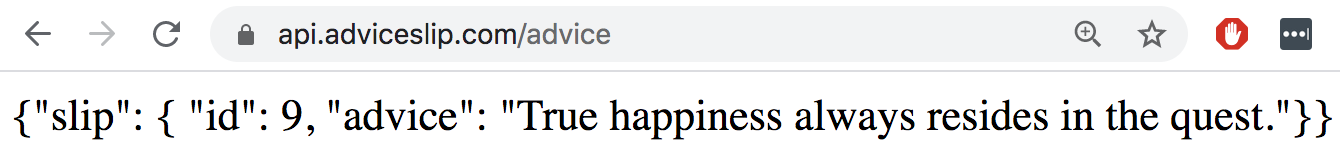
\includegraphics[width=0.8\linewidth]{images/api/advice-slip-happiness} 

}

\caption{Random advice from Advice Slip}\label{fig:unnamed-chunk-104}
\end{figure}

As you can tell, the content is a simple JSON string

\begin{Shaded}
\begin{Highlighting}[]
\NormalTok{advice\_url }\OtherTok{\textless{}{-}} \StringTok{"https://api.adviceslip.com/advice"}

\FunctionTok{fromJSON}\NormalTok{(advice\_url)}
\end{Highlighting}
\end{Shaded}

\begin{verbatim}
#> $slip
#> $slip$id
#> [1] 9
#> 
#> $slip$advice
#> [1] "True happiness always resides in the quest!"
\end{verbatim}

\hypertarget{example-colors-in-hexadecimal-notation}{%
\subsubsection*{Example: Colors in Hexadecimal Notation}\label{example-colors-in-hexadecimal-notation}}
\addcontentsline{toc}{subsubsection}{Example: Colors in Hexadecimal Notation}

The following data comes from one of Dave Eddy's github repositories:

\url{https://raw.githubusercontent.com/bahamas10/css-color-names/master/css-color-names.json}

This is a JSON-object in which the \emph{keys} are color-names, and the \emph{values} are
the hexadecimal digits of the corresponding color:

\begin{verbatim}
{
  "aliceblue": "#f0f8ff",
  "antiquewhite": "#faebd7",
  "aqua": "#00ffff",
  "aquamarine": "#7fffd4",
  "azure": "#f0ffff",
  ...
  "wheat": "#f5deb3",
  "white": "#ffffff",
  "whitesmoke": "#f5f5f5",
  "yellow": "#ffff00",
  "yellowgreen": "#9acd32"
}
\end{verbatim}

We pass the url to \texttt{jsonlite::fromJSON()}

\begin{Shaded}
\begin{Highlighting}[]
\NormalTok{colors\_json }\OtherTok{\textless{}{-}} \StringTok{"https://raw.githubusercontent.com/bahamas10/css{-}color{-}names/master/css{-}color{-}names.json"}

\NormalTok{hex\_colors }\OtherTok{\textless{}{-}} \FunctionTok{fromJSON}\NormalTok{(colors\_json)}
\end{Highlighting}
\end{Shaded}

The output in \texttt{hex\_colors} is a list with 148 elements;
the first five elements are displayed below:

\begin{Shaded}
\begin{Highlighting}[]
\NormalTok{hex\_colors[}\DecValTok{1}\SpecialCharTok{:}\DecValTok{5}\NormalTok{]}
\CommentTok{\#\textgreater{} $aliceblue}
\CommentTok{\#\textgreater{} [1] "\#f0f8ff"}
\CommentTok{\#\textgreater{} }
\CommentTok{\#\textgreater{} $antiquewhite}
\CommentTok{\#\textgreater{} [1] "\#faebd7"}
\CommentTok{\#\textgreater{} }
\CommentTok{\#\textgreater{} $aqua}
\CommentTok{\#\textgreater{} [1] "\#00ffff"}
\CommentTok{\#\textgreater{} }
\CommentTok{\#\textgreater{} $aquamarine}
\CommentTok{\#\textgreater{} [1] "\#7fffd4"}
\CommentTok{\#\textgreater{} }
\CommentTok{\#\textgreater{} $azure}
\CommentTok{\#\textgreater{} [1] "\#f0ffff"}
\end{Highlighting}
\end{Shaded}

\hypertarget{part-apis}{%
\part{APIs}\label{part-apis}}

\hypertarget{apis}{%
\chapter{Web APIs}\label{apis}}

In this chapter we'll give you a crash introduction to Web APIs, and how to
use R for interacting with them.

You will need the following packages

\begin{Shaded}
\begin{Highlighting}[]
\FunctionTok{library}\NormalTok{(httr2)}
\FunctionTok{library}\NormalTok{(xml2)}
\FunctionTok{library}\NormalTok{(jsonlite)}
\end{Highlighting}
\end{Shaded}

\hypertarget{introduction-1}{%
\section{Introduction}\label{introduction-1}}

So far we've been dealing with data sets in various formats: internal data
objects in R (e.g.~data tibble \texttt{starwars}), built-in data frames such as
\texttt{mtcars} or \texttt{oldfaithful}), reading files stored in your computer (txt, csv,
tsv, etc). But you also need to learn how to get data from the web.

For better or worse, reading data from the Web entails a whole other set of
considerations. Because of the large variety of data formats available in the
Web, we will primarily focus on retrieving data from
\emph{Application Programming Interfaces} also known as APIs.

The reason to focus on APIs is because nowadays many companies, websites,
sources, etc. use APIs as their primary means to share information and data.
Many large websites like Reddit, Twitter and Facebook offer APIs so that data
analysts and data scientists can access interesting data. And having an API to
share data has become a standard thing to have.

\hypertarget{a-little-bit-about-apis}{%
\section{A little bit about APIs}\label{a-little-bit-about-apis}}

API stands for \textbf{Application Programming Interface}. If this sounds too fancy
or cryptic for you, then simply think of it as a ``Data Sharing Interface''.

Instead of having to download a data file, an API allows programmers to request
data directly from a website. From a technical point of view, an API is a set
of rules, protocols, and tools for building software and applications.

\hypertarget{what-is-an-api}{%
\subsubsection*{What is an API?}\label{what-is-an-api}}
\addcontentsline{toc}{subsubsection}{What is an API?}

``API'' is a general term for the place where one computer program (the client)
interacts with another (the server), or with itself.

APIs offer data scientists a polished way to request clean and curated data
from a website. When a website like Facebook sets up an API, they are
essentially setting up a computer that waits for data requests.

Once this computer receives a data request, it will do its own processing of
the data and send it to the computer that requested it. From our perspective
as the requester, we will need to write code in R that creates the request and
tells the computer running the API what we need. That computer will then read
our code, process the request, and return nicely-formatted data that can be
easily parsed by existing R libraries.

\hypertarget{why-to-use-an-api}{%
\subsubsection*{Why to use an API?}\label{why-to-use-an-api}}
\addcontentsline{toc}{subsubsection}{Why to use an API?}

Why is this valuable? Contrast the API approach to pure web scraping. When a
programmer scrapes a web page, they receive the data in a messy chunk of HTML.
While there are certainly libraries out there that make parsing HTML text easy,
these are all cleaning steps that need to be taken before we even get our hands
on the data we want!

Often, we can immediately use the data we get from an API, which saves us time
and frustration.

\hypertarget{using-r-as-an-http-client}{%
\section{Using R as an HTTP Client}\label{using-r-as-an-http-client}}

R has a few HTTP client packages: \texttt{"crul"}, \texttt{"curl"}, \texttt{"httr2"}, and \texttt{"RCurl"};
you can think of them as ``high-level R HTTP clients'' which basically let you
use R (and your computer) as an \textbf{HTTP client}.

We will describe how to use functions from \texttt{"httr2"} (pronounced \emph{hitter2}).

\hypertarget{interacting-with-aps-via-r}{%
\section{Interacting with AP's via R}\label{interacting-with-aps-via-r}}

In R, we can use the \texttt{"httr2"} package to make http requests and handle the
responses.

Let's start with baby steps using the website \url{https://api.adviceslip.com/}
which provides an API to get a free piece of advice from the internet.

The first thing you need to do is to look at the web page to familiarize
yourself with the functionalities it provides.

\begin{figure}

{\centering 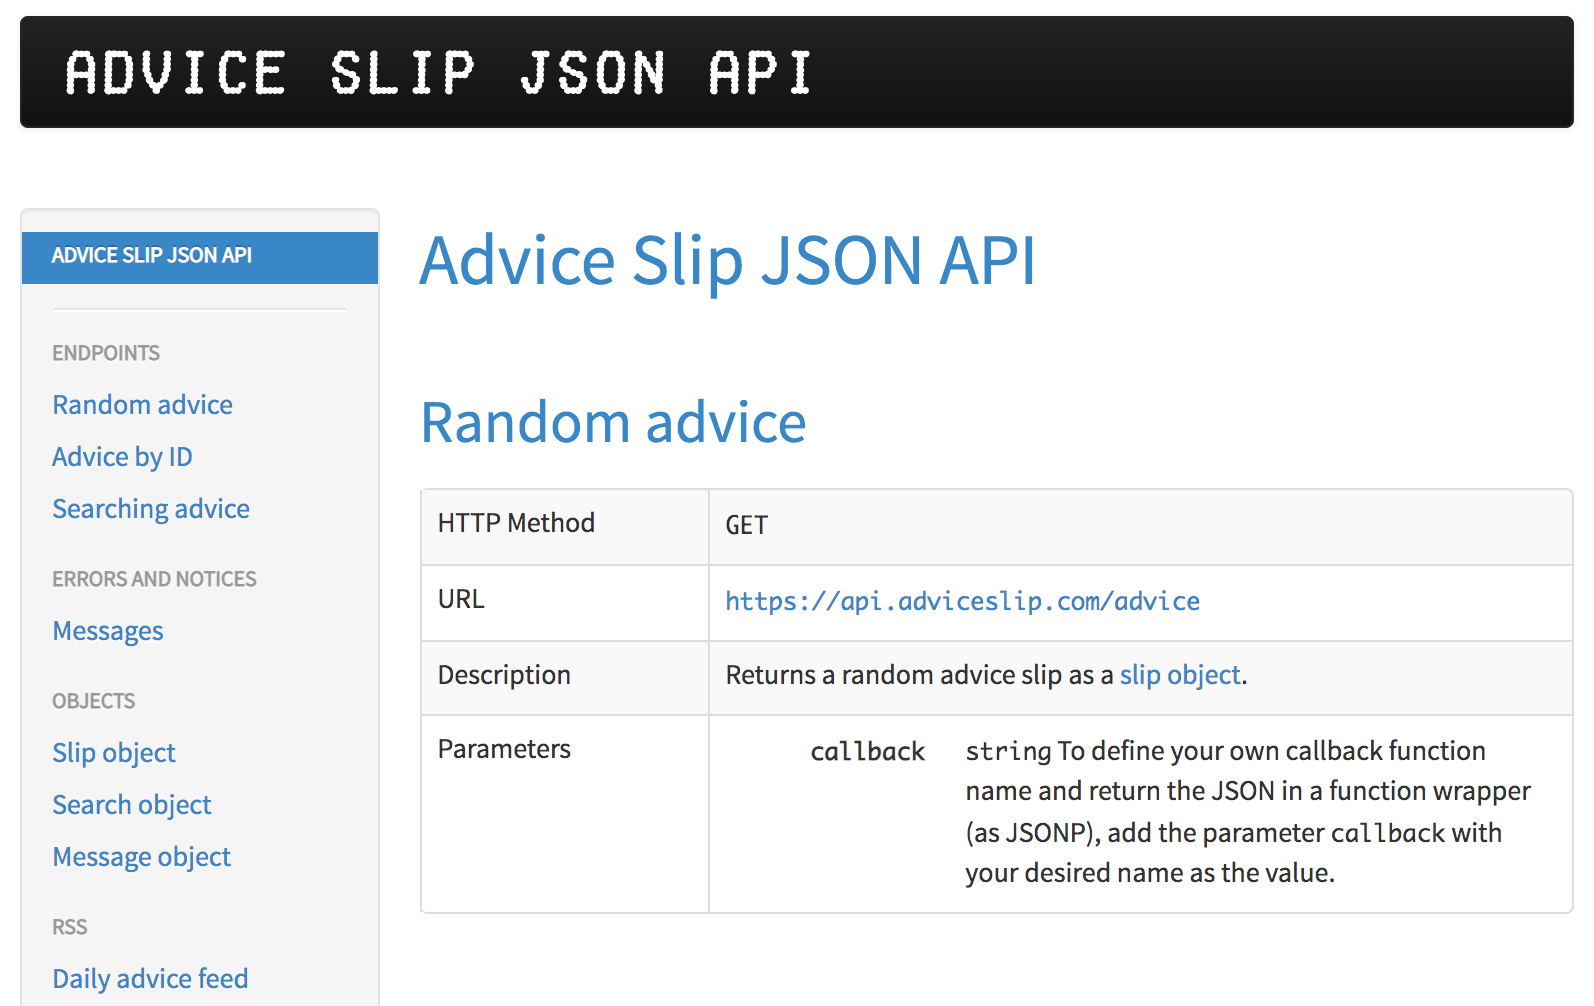
\includegraphics[width=0.75\linewidth]{images/api/advice-slip} 

}

\caption{Advice Slip JSON API}\label{fig:unnamed-chunk-113}
\end{figure}

The url \texttt{https://api.adviceslip.com/advice} will give you a random advice:

\begin{figure}

{\centering 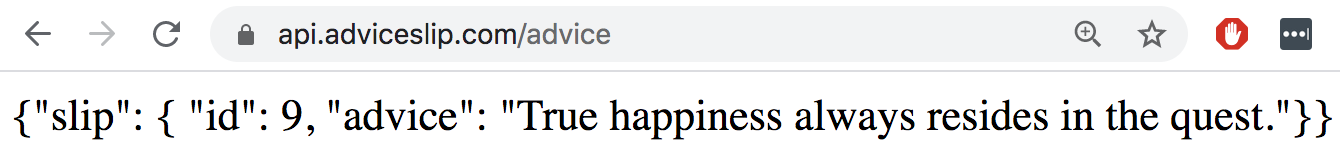
\includegraphics[width=0.75\linewidth]{images/api/advice-slip-happiness} 

}

\caption{Random advice from Advice Slip}\label{fig:unnamed-chunk-114}
\end{figure}

\hypertarget{making-request-from-r}{%
\subsection{Making request from R}\label{making-request-from-r}}

Notice that the format of the response is provided in JSON. In the above
example, the advice is given as:

\begin{verbatim}
{"slip": {"id": 9, "advice": "True happiness always resides in the quest."}}
\end{verbatim}

which we can mentally rearrange as:

\begin{verbatim}
{
  "slip": {
    "id": 9, 
    "advice": "True happiness always resides in the quest."
  }
}
\end{verbatim}

Getting a random advice is quite simple, all you need is to make an HTTP
request using the url \texttt{https://api.adviceslip.com/advice}.

Interestingly, we can make such request from R, using it as a server. This
requires employing some functions from \texttt{"httr2"}.

In \texttt{"httr2"}, you start by creating a \textbf{request}. How? You use the \texttt{request()}
function which creates a request object. To be clear, \texttt{request()} does not
submit the request, it only creates the object, which you can use to build up a
complex request piece by piece, and works well with the pipe operators \texttt{\textbar{}\textgreater{}}
or \texttt{\%\textgreater{}\%}.

\begin{Shaded}
\begin{Highlighting}[]
\CommentTok{\# start a request object}
\NormalTok{advice\_url }\OtherTok{=} \StringTok{"https://api.adviceslip.com"}
\NormalTok{req }\OtherTok{=} \FunctionTok{request}\NormalTok{(advice\_url)}
\NormalTok{req}
\CommentTok{\#\textgreater{} \textless{}httr2\_request\textgreater{}}
\CommentTok{\#\textgreater{} GET https://api.adviceslip.com}
\CommentTok{\#\textgreater{} Body: empty}
\end{Highlighting}
\end{Shaded}

To see what this request will send to the server we perform a dry run:

\begin{Shaded}
\begin{Highlighting}[]
\NormalTok{req }\SpecialCharTok{|\textgreater{}} \FunctionTok{req\_dry\_run}\NormalTok{()}
\CommentTok{\#\textgreater{} GET / HTTP/1.1}
\CommentTok{\#\textgreater{} Host: api.adviceslip.com}
\CommentTok{\#\textgreater{} User{-}Agent: httr2/1.0.0 r{-}curl/5.1.0 libcurl/7.79.1}
\CommentTok{\#\textgreater{} Accept: */*}
\CommentTok{\#\textgreater{} Accept{-}Encoding: deflate, gzip}
\end{Highlighting}
\end{Shaded}

What's going on with the first line \texttt{GET\ /\ HTTP/1.1}?

\begin{itemize}
\item
  The first term, \texttt{GET}, refers to the HTTP \textbf{method}, which is a
  verb that tells the server what you want to do. In this case is \texttt{GET}, the most
  common verb, indicating that we want to get a resource. Other verbs include
  \texttt{POST}, to create a new resource; \texttt{PUT}, to replace an existing resource; and
  \texttt{DELETE}, to delete a resource.
\item
  The second part, \texttt{/}, is the \textbf{path} which is the URL stripped of details
  that the server already knows, i.e.~the protocol (http or https), and the host
  (localhost).
\item
  The third element, \texttt{HTTP/1.1}, is the version of the HTTP protocol. This is
  unimportant for our purposes because it's handled at a lower level.
\end{itemize}

In order to make a request with \texttt{"httr2"}, we need to complete the full path
of the URL. In the above example, this is done with \texttt{req\_url\_path\_append()}

\begin{Shaded}
\begin{Highlighting}[]
\CommentTok{\# then we complete the full path}
\NormalTok{req }\SpecialCharTok{|\textgreater{}}
  \FunctionTok{req\_url\_path\_append}\NormalTok{(}\StringTok{"advice"}\NormalTok{) }
\CommentTok{\#\textgreater{} \textless{}httr2\_request\textgreater{}}
\CommentTok{\#\textgreater{} GET https://api.adviceslip.com/advice}
\CommentTok{\#\textgreater{} Body: empty}
\end{Highlighting}
\end{Shaded}

\hypertarget{performing-a-request}{%
\subsection{Performing a Request}\label{performing-a-request}}

Once we have the desired request object, then we can submit it or \textbf{perform}
such request with \texttt{req\_perform()}:

\begin{Shaded}
\begin{Highlighting}[]
\CommentTok{\# then add on the query path}
\NormalTok{resp }\OtherTok{=}\NormalTok{ req }\SpecialCharTok{|\textgreater{}}
  \FunctionTok{req\_url\_path\_append}\NormalTok{(}\StringTok{"advice"}\NormalTok{) }\SpecialCharTok{|\textgreater{}}
  \FunctionTok{req\_perform}\NormalTok{()}

\NormalTok{resp}
\CommentTok{\#\textgreater{} \textless{}httr2\_response\textgreater{}}
\CommentTok{\#\textgreater{} GET https://api.adviceslip.com/advice}
\CommentTok{\#\textgreater{} Status: 200 OK}
\CommentTok{\#\textgreater{} Content{-}Type: text/html}
\CommentTok{\#\textgreater{} Body: In memory (77 bytes)}
\end{Highlighting}
\end{Shaded}

As you can tell, the response has a success status (\texttt{200\ OK}), and the fetched
content is text in html format.

The object \texttt{resp} is an object of class \texttt{"httr2\_response"}, which is basically
an R list that contains 7 elements:

\begin{Shaded}
\begin{Highlighting}[]
\FunctionTok{names}\NormalTok{(resp)}
\CommentTok{\#\textgreater{} [1] "method"      "url"         "status\_code" "headers"     "body"       }
\CommentTok{\#\textgreater{} [6] "request"     "cache" }
\end{Highlighting}
\end{Shaded}

As you can tell, one of the elements in \texttt{resp} is \texttt{"body"}. If we take a look
at the body we get an interesting---but unhelpful---output:

\begin{Shaded}
\begin{Highlighting}[]
\NormalTok{resp}\SpecialCharTok{$}\NormalTok{body}
\CommentTok{\#\textgreater{}  [1] 7b 22 73 6c 69 70 22 3a 20 7b 20 22 69 64 22 3a 20 39 2c 20 22 61 64 76}
\CommentTok{\#\textgreater{} [25] 69 63 65 22 3a 20 22 54 72 75 65 20 68 61 70 70 69 6e 65 73 73 20 61 6c}
\CommentTok{\#\textgreater{} [49] 77 61 79 73 20 72 65 73 69 64 65 73 20 69 6e 20 74 68 65 20 71 75 65 73}
\CommentTok{\#\textgreater{} [73] 74 2e 22 7d 7d}
\end{Highlighting}
\end{Shaded}

What kind of object is \texttt{resp\$body}? Inspecting its \texttt{class()}, it turns out
that this is an object of class \texttt{"raw"} or \emph{raw vector}, which is a vector
that holds raw bytes in R.

\begin{Shaded}
\begin{Highlighting}[]
\FunctionTok{class}\NormalTok{(resp}\SpecialCharTok{$}\NormalTok{body)}
\CommentTok{\#\textgreater{} [1] "raw"}
\end{Highlighting}
\end{Shaded}

Technically speaking, a raw vector is printed with each byte separately
represented as a pair of hex digits. If you want to see a character
representation (with escape sequences for non-printing characters) use
\texttt{rawToChar()}.

\begin{Shaded}
\begin{Highlighting}[]
\NormalTok{body\_json }\OtherTok{=} \FunctionTok{rawToChar}\NormalTok{(resp}\SpecialCharTok{$}\NormalTok{body)}

\NormalTok{body\_json}
\CommentTok{\#\textgreater{} [1] "\{\textbackslash{}"slip\textbackslash{}": \{ \textbackslash{}"id\textbackslash{}": 9, \textbackslash{}"advice\textbackslash{}": \textbackslash{}"True happiness always resides in the quest.\textbackslash{}"\}\}"}
\end{Highlighting}
\end{Shaded}

Converting the raw vector into text, we obtain the response body \texttt{body\_json}
which is text in JSON format. Then, to parse this JSON text, we use \texttt{fromJSON()}
which returns an R list:

\begin{Shaded}
\begin{Highlighting}[]
\NormalTok{slip\_advice }\OtherTok{=} \FunctionTok{fromJSON}\NormalTok{(body\_json)}

\NormalTok{slip\_advice}
\CommentTok{\#\textgreater{} $slip}
\CommentTok{\#\textgreater{} $slip$id}
\CommentTok{\#\textgreater{} [1] 9}

\CommentTok{\#\textgreater{} $slip$advice}
\CommentTok{\#\textgreater{} [1] "True happiness always resides in the quest."}
\end{Highlighting}
\end{Shaded}

And finally, we extract the piece of advice as follows:

\begin{Shaded}
\begin{Highlighting}[]
\NormalTok{slip\_advice}\SpecialCharTok{$}\NormalTok{slip}\SpecialCharTok{$}\NormalTok{advice}
\CommentTok{\#\textgreater{} [1] "True happiness always resides in the quest."}
\end{Highlighting}
\end{Shaded}

\hypertarget{extracting-response-as-string}{%
\subsection{Extracting response as string}\label{extracting-response-as-string}}

Let me show you another more straightforward way to extract the content of the
response body by using one the \texttt{resp\_body\_()} functions, in particular the
\texttt{resp\_body\_string()} function:

\begin{Shaded}
\begin{Highlighting}[]
\NormalTok{resp }\SpecialCharTok{|\textgreater{}} \FunctionTok{resp\_body\_string}\NormalTok{()}
\CommentTok{\#\textgreater{} [1] "\{\textbackslash{}"slip\textbackslash{}": \{ \textbackslash{}"id\textbackslash{}": 9, \textbackslash{}"advice\textbackslash{}": \textbackslash{}"True happiness always resides in the quest.\textbackslash{}"\}\}"}
\end{Highlighting}
\end{Shaded}

Notice that we obtain the same JSON text, which we can parse with \texttt{fromJSON()}

\begin{Shaded}
\begin{Highlighting}[]
\NormalTok{resp }\SpecialCharTok{|\textgreater{}} \FunctionTok{resp\_body\_string}\NormalTok{() }\SpecialCharTok{|\textgreater{}} \FunctionTok{fromJSON}\NormalTok{()}
\CommentTok{\#\textgreater{} $slip}
\CommentTok{\#\textgreater{} $slip$id}
\CommentTok{\#\textgreater{} [1] 9}

\CommentTok{\#\textgreater{} $slip$advice}
\CommentTok{\#\textgreater{} [1] "True happiness always resides in the quest."}
\end{Highlighting}
\end{Shaded}

\hypertarget{extracting-response-as-html}{%
\subsection{Extracting response as HTML}\label{extracting-response-as-html}}

A third equivalent method to extract the response body is with the function
\texttt{resp\_body\_html()}. The reason shy we can do that in this case has to do with
the fact that the content of the response is in HTML format:
\texttt{Content-Type:\ text/html}.

\begin{Shaded}
\begin{Highlighting}[]
\CommentTok{\# the result comes back as html}
\CommentTok{\# Let\textquotesingle{}s extract body from response}
\NormalTok{doc\_html }\OtherTok{=}\NormalTok{ resp }\SpecialCharTok{|\textgreater{}} \FunctionTok{resp\_body\_html}\NormalTok{()}

\NormalTok{doc\_html}
\CommentTok{\#\textgreater{} \{html\_document\}}
\CommentTok{\#\textgreater{} \textless{}html\textgreater{}}
\CommentTok{\#\textgreater{} [1] \textless{}body\textgreater{}\textless{}p\textgreater{}\{"slip": \{ "id": 9, "advice": "True happiness always resides ...}
\end{Highlighting}
\end{Shaded}

Since the output is an \texttt{html\_document}, we first need to extract the text of
the \texttt{\textless{}p\textgreater{}} element. One option to achieve this is some xpath expression:

\begin{Shaded}
\begin{Highlighting}[]
\NormalTok{txt\_json }\OtherTok{=}\NormalTok{ doc\_html }\SpecialCharTok{|\textgreater{}} 
  \FunctionTok{xml\_find\_all}\NormalTok{(}\AttributeTok{xpath =} \StringTok{"//p"}\NormalTok{) }\SpecialCharTok{|\textgreater{}}
  \FunctionTok{xml\_text}\NormalTok{()}

\NormalTok{txt\_json}
\CommentTok{\#\textgreater{} [1] "\{\textbackslash{}"slip\textbackslash{}": \{ \textbackslash{}"id\textbackslash{}": 9, \textbackslash{}"advice\textbackslash{}": \textbackslash{}"True happiness always resides in the quest.\textbackslash{}"\}\}"}
\end{Highlighting}
\end{Shaded}

This still requires some JSON manipulation:

\begin{Shaded}
\begin{Highlighting}[]
\NormalTok{slip\_advice }\OtherTok{=} \FunctionTok{fromJSON}\NormalTok{(txt\_json)}
\NormalTok{slip\_advice}
\CommentTok{\#\textgreater{} $slip}
\CommentTok{\#\textgreater{} $slip$id}
\CommentTok{\#\textgreater{} [1] 9}

\CommentTok{\#\textgreater{} $slip$advice}
\CommentTok{\#\textgreater{} [1] "True happiness always resides in the quest."}
\end{Highlighting}
\end{Shaded}

\hypertarget{example-search-with-advice-id}{%
\section{Example: Search with Advice ID}\label{example-search-with-advice-id}}

The Advice Slip API also allows you to request an advice based on its ID.

\begin{figure}

{\centering 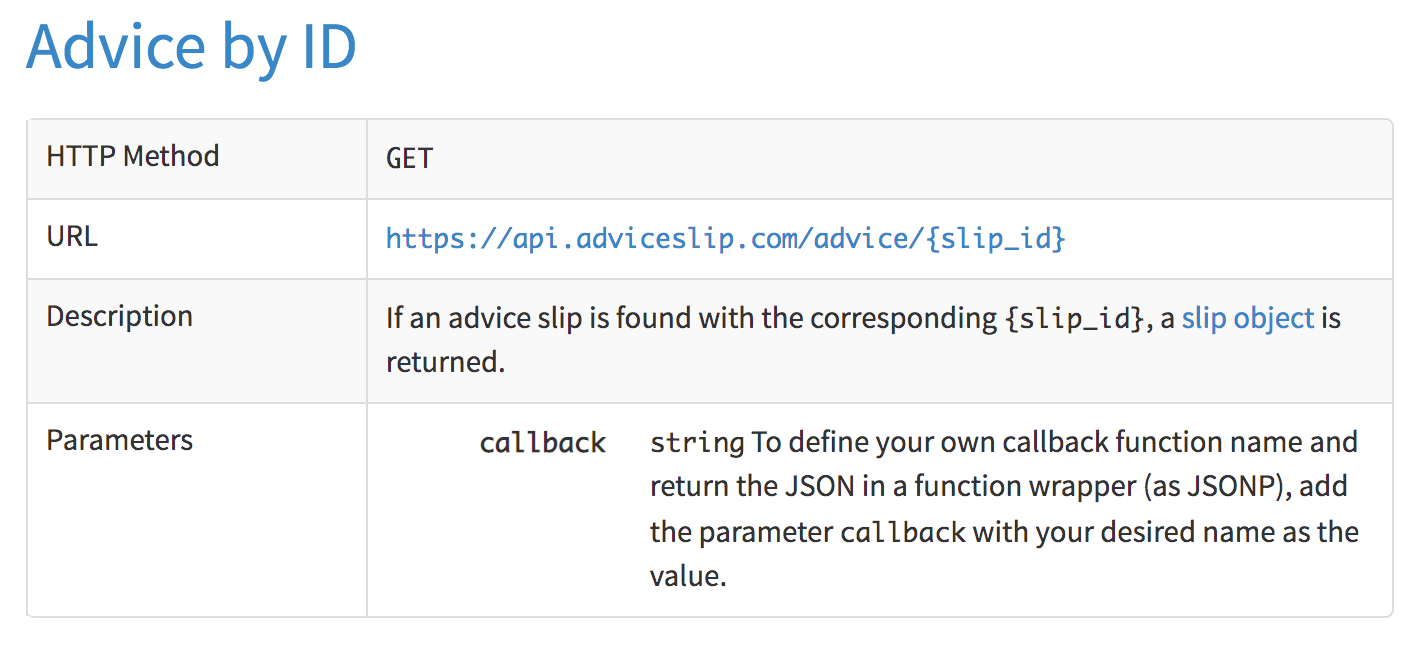
\includegraphics[width=0.75\linewidth]{images/api/advice-slip-by-id} 

}

\caption{Random advices by id}\label{fig:unnamed-chunk-130}
\end{figure}

For example, the id = 5 results in the following advice:

\begin{figure}

{\centering 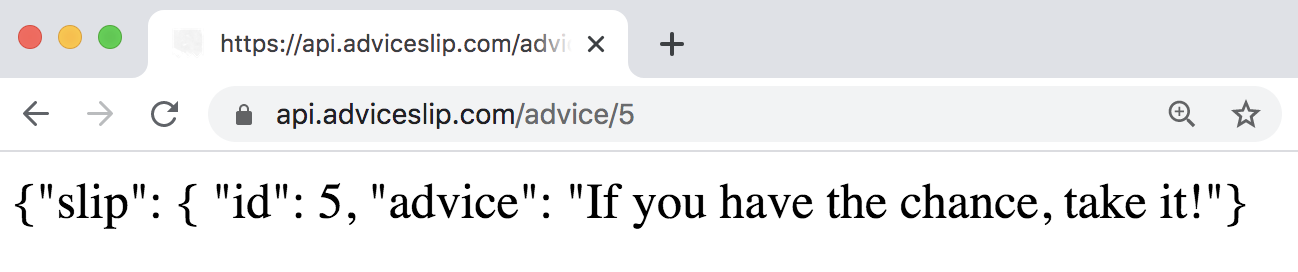
\includegraphics[width=0.7\linewidth]{images/api/advice-slip-id5} 

}

\caption{Random advice from Advice Slip}\label{fig:unnamed-chunk-131}
\end{figure}

To make this request from R, we create the request object, and then perform
such request

\begin{Shaded}
\begin{Highlighting}[]
\CommentTok{\# advice id=5}
\NormalTok{resp\_advice\_id5 }\OtherTok{\textless{}{-}}\NormalTok{ req }\SpecialCharTok{|\textgreater{}}
  \FunctionTok{req\_url\_path\_append}\NormalTok{(}\StringTok{"advice/5"}\NormalTok{) }\SpecialCharTok{|\textgreater{}}
  \FunctionTok{req\_perform}\NormalTok{()}

\NormalTok{resp\_advice\_id5}
\CommentTok{\#\textgreater{} \textless{}httr2\_response\textgreater{}}
\CommentTok{\#\textgreater{} GET https://api.adviceslip.com/advice/5}
\CommentTok{\#\textgreater{} Status: 200 OK}
\CommentTok{\#\textgreater{} Content{-}Type: text/html}
\CommentTok{\#\textgreater{} Body: In memory (66 bytes)}
\end{Highlighting}
\end{Shaded}

We can then extract the response body, for instance:

\begin{Shaded}
\begin{Highlighting}[]
\NormalTok{advice\_id5 }\OtherTok{=}\NormalTok{ resp\_advice\_id5 }\SpecialCharTok{|\textgreater{}} \FunctionTok{resp\_body\_string}\NormalTok{() }\SpecialCharTok{|\textgreater{}} \FunctionTok{fromJSON}\NormalTok{()}
\NormalTok{advice\_id5}
\CommentTok{\#\textgreater{} $slip}
\CommentTok{\#\textgreater{} $slip$id}
\CommentTok{\#\textgreater{} [1] 5}

\CommentTok{\#\textgreater{} $slip$advice}
\CommentTok{\#\textgreater{} [1] "If you have the chance, take it!"}
\end{Highlighting}
\end{Shaded}

\hypertarget{example-search-query}{%
\section{Example: Search Query}\label{example-search-query}}

Another kind of request that you can do with the Advice Slip API is to search
for an advice specifying a search query:

\begin{figure}

{\centering 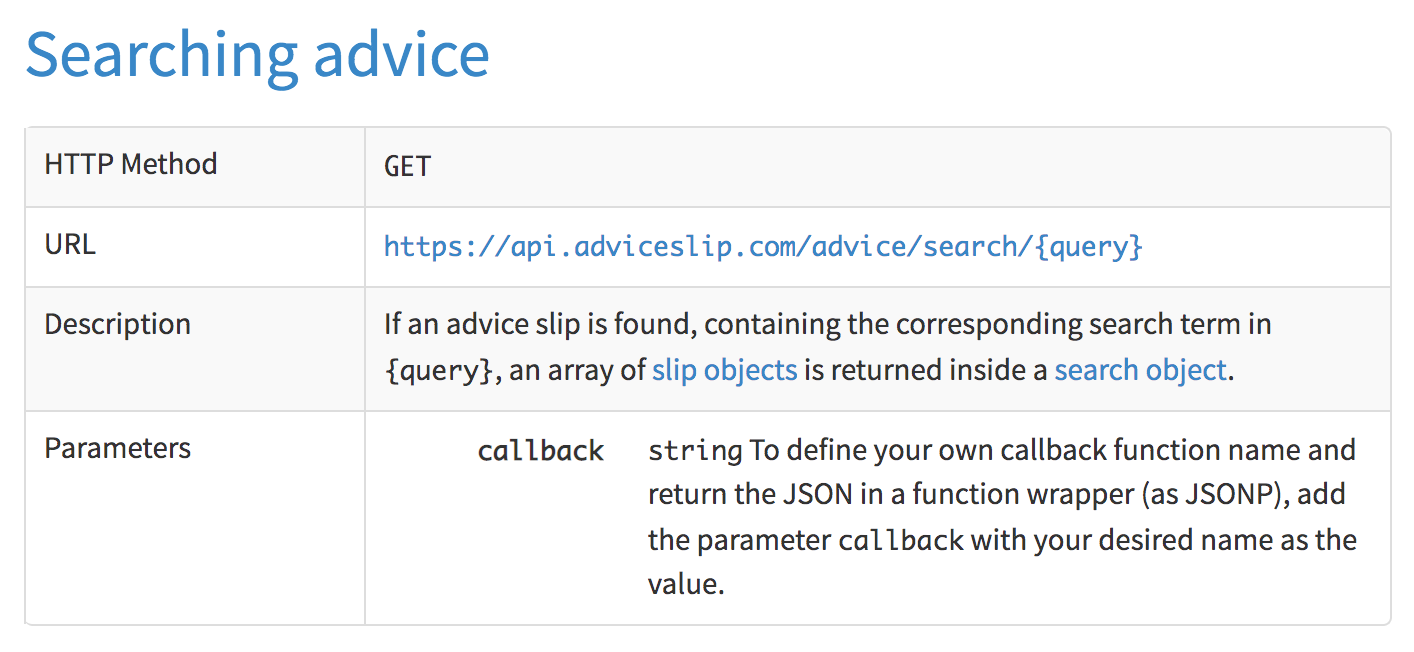
\includegraphics[width=0.7\linewidth]{images/api/advice-slip-search} 

}

\caption{Random advices with search query}\label{fig:unnamed-chunk-134}
\end{figure}

For example, say we are interested in searching for advice that includes the
word \textbf{chance}. The corresponding URL path will have the following form:

\texttt{https://api.adviceslip.com/advice/search/chance}

\begin{figure}

{\centering 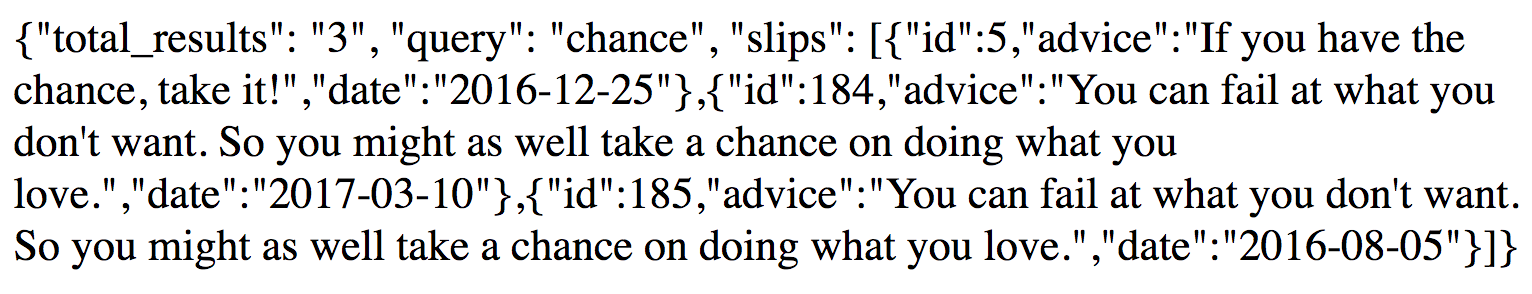
\includegraphics[width=0.75\linewidth]{images/api/advice-slip-chance} 

}

\caption{Random advices with search query 'chance'}\label{fig:unnamed-chunk-135}
\end{figure}

Let's search for the term \texttt{chance}. For sake of illustration, let's build a
request object by appending the path elements: \texttt{advice}, \texttt{search}, and \texttt{chance}

\begin{Shaded}
\begin{Highlighting}[]
\CommentTok{\# advice id=5}
\NormalTok{resp\_advice\_chance }\OtherTok{\textless{}{-}}\NormalTok{ req }\SpecialCharTok{|\textgreater{}}
  \FunctionTok{req\_url\_path\_append}\NormalTok{(}\StringTok{"advice"}\NormalTok{) }\SpecialCharTok{|\textgreater{}}
  \FunctionTok{req\_url\_path\_append}\NormalTok{(}\StringTok{"search"}\NormalTok{) }\SpecialCharTok{|\textgreater{}}
  \FunctionTok{req\_url\_path\_append}\NormalTok{(}\StringTok{"chance"}\NormalTok{) }\SpecialCharTok{|\textgreater{}}
  \FunctionTok{req\_perform}\NormalTok{()}
\end{Highlighting}
\end{Shaded}

The above command can be shorten as:

\begin{Shaded}
\begin{Highlighting}[]
\CommentTok{\# advice id=5}
\NormalTok{resp\_advice\_chance }\OtherTok{\textless{}{-}}\NormalTok{ req }\SpecialCharTok{|\textgreater{}}
  \FunctionTok{req\_url\_path\_append}\NormalTok{(}\StringTok{"advice/search/chance"}\NormalTok{) }\SpecialCharTok{|\textgreater{}}
  \FunctionTok{req\_perform}\NormalTok{()}

\NormalTok{resp\_advice\_chance}
\CommentTok{\#\textgreater{} \textless{}httr2\_response\textgreater{}}
\CommentTok{\#\textgreater{} GET https://api.adviceslip.com/advice/search/chance}
\CommentTok{\#\textgreater{} Status: 200 OK}
\CommentTok{\#\textgreater{} Content{-}Type: text/html}
\CommentTok{\#\textgreater{} Body: In memory (402 bytes)}
\end{Highlighting}
\end{Shaded}

Having performed the request, we fetch the data by extracting the body as a
string (in JSON format), and then parsing with \texttt{fromJSON()}

\begin{Shaded}
\begin{Highlighting}[]
\NormalTok{advice\_chance }\OtherTok{=}\NormalTok{ resp\_advice\_chance }\SpecialCharTok{|\textgreater{}} \FunctionTok{resp\_body\_string}\NormalTok{() }\SpecialCharTok{|\textgreater{}} \FunctionTok{fromJSON}\NormalTok{()}

\FunctionTok{names}\NormalTok{(advice\_chance)}
\CommentTok{\#\textgreater{} [1] "total\_results" "query"         "slips" }
\end{Highlighting}
\end{Shaded}

The \texttt{"slips"} element contains a data frame with 3 advice recommendations:

\begin{Shaded}
\begin{Highlighting}[]
\NormalTok{advice\_chance}\SpecialCharTok{$}\NormalTok{slips}
\CommentTok{\#\textgreater{}    id}
\CommentTok{\#\textgreater{} 1   5}
\CommentTok{\#\textgreater{} 2 184}
\CommentTok{\#\textgreater{} 3 185}
\CommentTok{\#\textgreater{}                                                                                            advice}
\CommentTok{\#\textgreater{} 1                                                                If you have the chance, take it!}
\CommentTok{\#\textgreater{} 2 You can fail at what you don\textquotesingle{}t want. So you might as well take a chance on doing what you love.}
\CommentTok{\#\textgreater{} 3 You can fail at what you don\textquotesingle{}t want. So you might as well take a chance on doing what you love.}
\CommentTok{\#\textgreater{}         date}
\CommentTok{\#\textgreater{} 1 2016{-}12{-}25}
\CommentTok{\#\textgreater{} 2 2017{-}03{-}10}
\CommentTok{\#\textgreater{} 3 2016{-}08{-}05}
\end{Highlighting}
\end{Shaded}

\hypertarget{api-pubmed}{%
\chapter{PubMed API Example}\label{api-pubmed}}

In this chapter, we provide an example of web data collection from the database
PubMed, using the \textbf{Entrez Programming Utilities}, commonly referred to as
E-utilities, from the National Center for Biotechnology Information (NCBI).

You will need the following packages:

\begin{Shaded}
\begin{Highlighting}[]
\FunctionTok{library}\NormalTok{(stringr)    }\CommentTok{\# for strings and regular expressions}
\FunctionTok{library}\NormalTok{(xml2)       }\CommentTok{\# for parsing data in XML (e.g. HTML)}
\FunctionTok{library}\NormalTok{(rvest)      }\CommentTok{\# for scraping XML and HTML content}
\FunctionTok{library}\NormalTok{(tm)         }\CommentTok{\# for text mining}
\FunctionTok{library}\NormalTok{(wordcloud2) }\CommentTok{\# for graphing wordclouds (optional)}
\end{Highlighting}
\end{Shaded}

\hypertarget{pubmed}{%
\section{PubMed}\label{pubmed}}

\textbf{PubMed} (\url{https://www.pubmed.gov}) is a database of the largest collection of
citations to medical journal literature in the world, and it is one of 38
databases built and maintained by the NCBI. Scientists, researchers, and users
around the world use PubMed to search and retrieve bibliographic data, choose
from several display formats, and share their results. Keep in mind that when
people talk about PubMed, they could be referring to both the search interface
and to the database itself.

PubMed's website provides a search engine to obtain bibliographic information:

\begin{figure}

{\centering 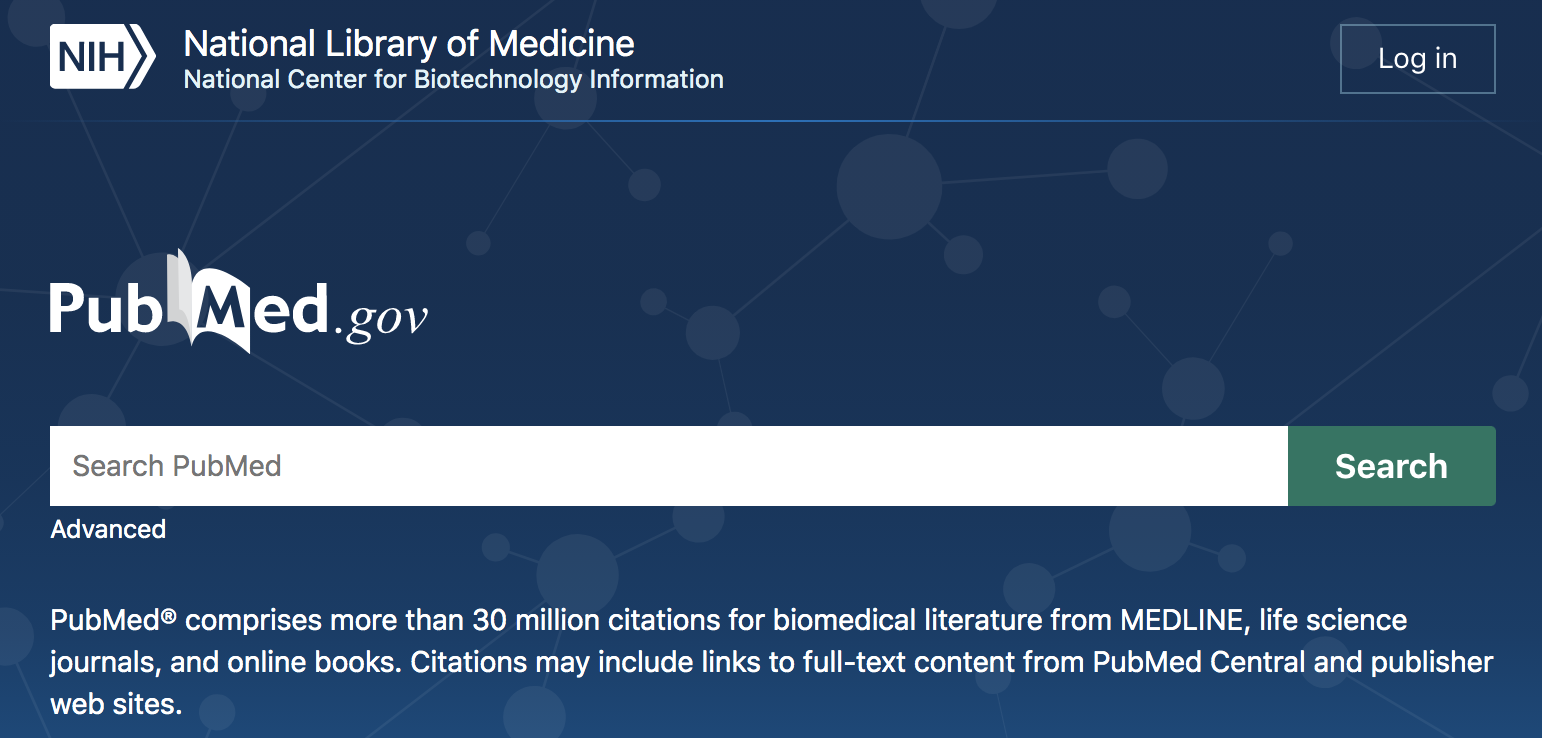
\includegraphics[width=0.7\linewidth]{images/api/pubmed-homepage} 

}

\caption{Partial screenshot of PubMed's homepage}\label{fig:unnamed-chunk-143}
\end{figure}

The simplest use of PubMed's search engine is to provide a query, very similar
to the queries that you would provide to google's search engine. For example,
we may be interested in looking for articles and other publications associated
with some of the effects that exposure to Bisphenol A (BPA) has on reproductive
health. Therefore, we can type in \texttt{BPA\ exposure\ reproductive\ health} inside the
search box, and obtain some results (like those displayed in the screenshot
below).

\begin{figure}

{\centering 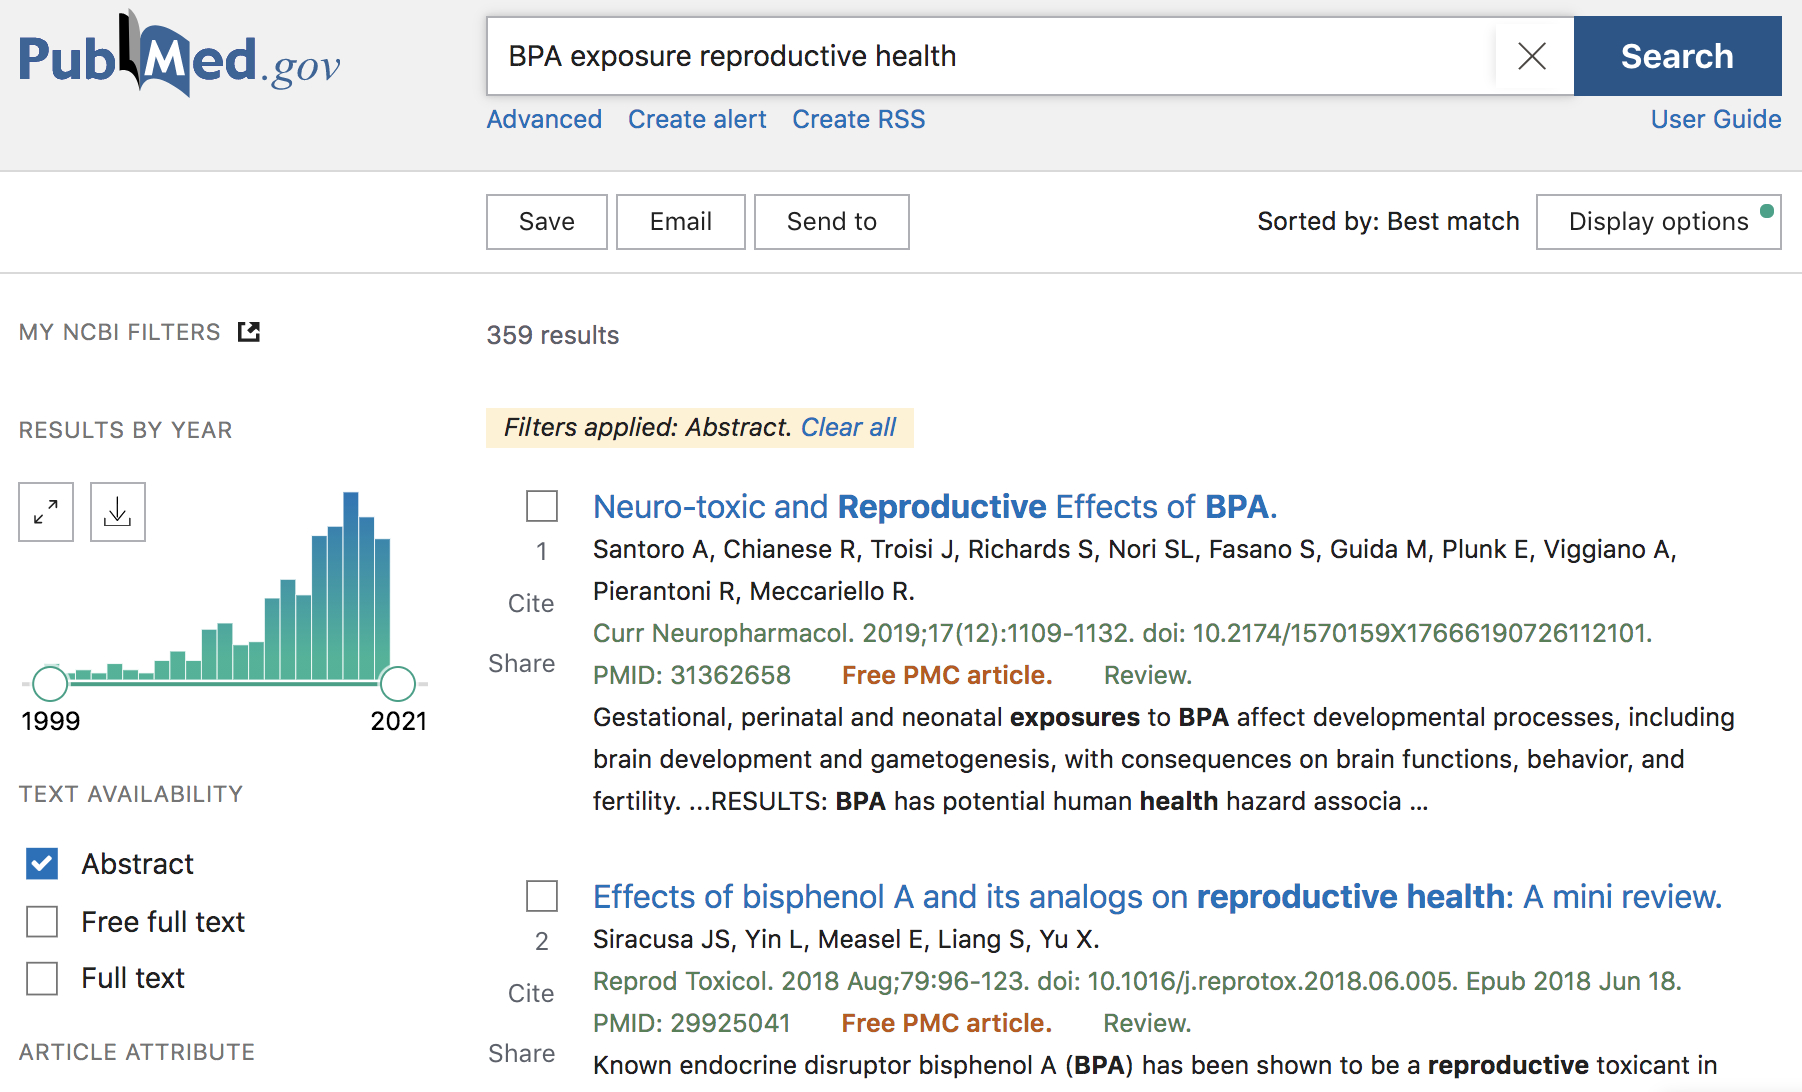
\includegraphics[width=0.7\linewidth]{images/api/pubmed-search1} 

}

\caption{PubMed search example}\label{fig:unnamed-chunk-144}
\end{figure}

As of this writing (Fall 2020), there are 359 results that match the query
term, with publications ranging from 1999 to end-of-2020. Notice that the
webpage has a sidebar with checkboxes, and other intereactive options, that
allow you to filter results by year of publication, by searching for the query
in the abstract, or just in the titles, and things like that. As an example,
we can move the slider for the year of publication to retrieve results that
were published in 2018 and 2019 (see screenshot below)

\begin{figure}

{\centering 
\includegraphics[width=0.7\linewidth]{images/api/pubmed-search2} 

}

\caption{PubMed search example (cont'd)}\label{fig:unnamed-chunk-145}
\end{figure}

If the obtained results are what you were looking for, you also have the option
to download a CSV file with such results (download button in the navigation bar,
above the barchart of years of publication).

In addition, you can perform a more advanced search by clicking on the
``Advanced'' button displayed below the search box. Clicking on this option
will take you to a new page with more query boxes and a long list of query
fields (screenshot below).

\begin{figure}

{\centering 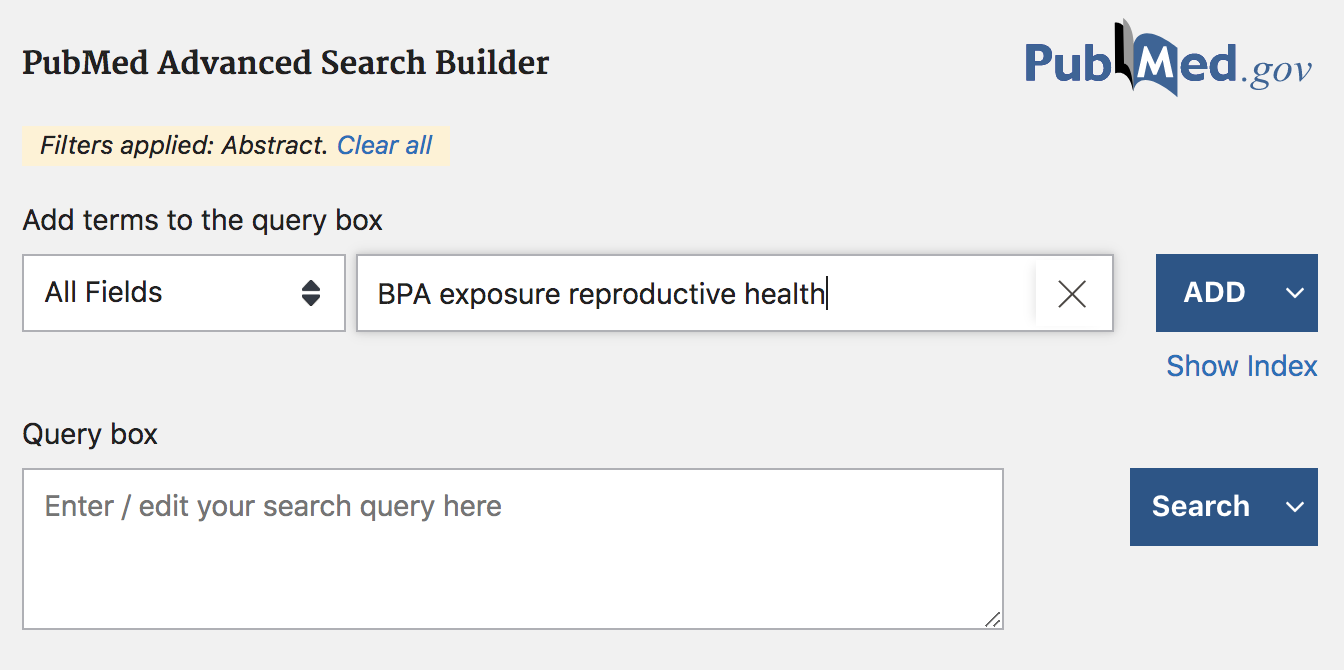
\includegraphics[width=0.7\linewidth]{images/api/pubmed-search3} 

}

\caption{PubMed search example (cont'd)}\label{fig:unnamed-chunk-146}
\end{figure}

In the Advanced search mode, you can find a large list of fields that give you
the opportunity to specify a more detailed query. For example, you can be more
specific in your search by looking for results based on title, or based on
author(s) information, or by date of publication, etc.

This way of interacting with PubMed (and similar databases) is how most
users and researchers utilize PubMed: performing manual searches through their
browsers, obtaining the results on their screens, and deciding which
publications are worth further inspection. Sometimes, however, you may:

\begin{itemize}
\item
  have a question that cannot be answered easily when you search PubMed,
\item
  need to see every citation in PubMed in a certain field,
\item
  need to run a search in PubMed and get the output in a CSV file that
  includes more (or different) data elements than the standard CSV file,
\item
  need to run specialized queries that might serve a very specific research
  need.
\end{itemize}

This is where \textbf{E-utilities} comes very handy because you can obtain the data
that you need, and only the data that you need, in the format that you need.
E-utilities is a great solution when you:

\begin{itemize}
\item
  can't find a good way to ask your question using the PubMed search box.
\item
  can search PubMed, but you'd like more, or less, or different data returned
  from the records.
\item
  want more control over the format of your PubMed data.
\end{itemize}

E-utilities is simply another way to search PubMed and the other NCBI databases.
Formally, E-utilities is an Application Programming Interface (API) which allows
you to control exactly what fields you are searching, the specific data
elements you retrieve, the format of the data, and how you share your results.
When you use E-utilities to access PubMed, you are accessing the same
data that you would find at \url{https://www.pubmed.gov}.

\hypertarget{basics-of-e-utilities}{%
\section{Basics of E-utilities}\label{basics-of-e-utilities}}

E-utilities is the short name for the \textbf{Entrez Programming Utilities}, which
is simply another way to search PubMed and other NCBI databases. The
E-utilities website is:

https://www.ncbi.nlm.nih.gov/books/NBK25500/

which contains the official documentation, written and maintained by Eric Sayers.

According to the website:

\begin{quote}
``Entrez Programming Utilities (E-utilities) are a set of nine server-side
programs that provide a stable interface into the Entrez query and database
system at the National Center for Biotechnology Information (NCBI).''
\end{quote}

What does this mean? E-utilities is basically an Application Programming
Interface (API). The E-utilities API allows you to search PubMed and any other
NCBI database through your own program: e.g.~R, Python, etc. When you use
E-utilities to access PubMed, you are accessing the same data that you'd find
at \url{https://www.pubmed.gov}.

\emph{Note}: the results returned by E-utilities queries of PubMed may differ
slightly from those returned in the web version of PubMed. As of this writing
(Fall 2020) a new PubMed API is currently under development.

\hypertarget{the-nine-e-utilities}{%
\subsubsection*{The Nine E-utilities}\label{the-nine-e-utilities}}
\addcontentsline{toc}{subsubsection}{The Nine E-utilities}

The name \emph{E-utilities} comes from the nine utilities (or programs):

\begin{itemize}
\item
  \textbf{EInfo} (database statistics): Provides the number of records indexed in each field of a given database, the date of the last update of the database, and the available links from the database to other Entrez databases.
\item
  \textbf{ESearch} (database statistics): Responds to a text query with the list of matching UIDs in a given database (for later use in ESummary, EFetch or ELink), along with the term translations of the query.
\item
  \textbf{EPost} (UID uploads): Accepts a list of UIDs from a given database, stores the set on the History Server, and responds with a query key and web environment for the uploaded dataset.
\item
  \textbf{ESummary} (document summary downloads): Responds to a list of UIDs from a given database with the corresponding document summaries.
\item
  \textbf{EFetch} (data record downloads): Responds to a list of UIDs in a given database with the corresponding data records in a specified format.
\item
  \textbf{ELink} (Entrez links): Responds to a list of UIDs in a given database with either a list of related UIDs (and relevancy scores) in the same database or a list of linked UIDs in another Entrez database
\item
  \textbf{EGQuery} (global query): Responds to a text query with the number of records matching the query in each Entrez database.
\item
  \textbf{ESpell} (spelling suggestions): Retrieves spelling suggestions for a text query in a given database.
\item
  \textbf{ECitMatch} (batch citation searching in PubMed): Retrieves PubMed IDs (PMIDs) corresponding to a set of input citation strings.
\end{itemize}

\textbf{For illustration purposes, we will only focus on ESearch, ESummary, and EFetch.}

\hypertarget{how-does-e-utilities-work}{%
\subsection{How does E-utilities work?}\label{how-does-e-utilities-work}}

The way you use E-utilities is by assembling an e-utilities URL, following
a specific set of rules, that you can use to make a request to one of its nine
servers.

Behind the scenes, the assembled E-utilities URL is translated into a standard
set of input parameters that are used as the values necessary for various NCBI
software components to search for and retrieve the requested data.
In other words, the URLs direct requests to servers that are used only by the
E-utilities and that are optimized to give users the best performance.

Before making any requests, keep in mind the following recommendation:

\begin{quote}
``In order not to overload the E-utility servers, NCBI recommends that users
post no more than three URL requests per second and limit large jobs to
either weekends or between 9:00 PM and 5:00 AM Eastern time during weekdays.''
\end{quote}

By the way, you can obtain an API Key offering you enhanced levels of supported
access to the E-utilities. This is totally optional but worth knowing. In our
examples, we won't need an API key, but if you plan to use PubMed more intensively
then consider getting an API Key.

\hypertarget{api-requests}{%
\subsubsection*{API Requests}\label{api-requests}}
\addcontentsline{toc}{subsubsection}{API Requests}

To make requests, you have to assemble a URL. Each URL consists of three parts:

\begin{enumerate}
\def\labelenumi{\arabic{enumi})}
\item
  \textbf{The base URL}: This is the address of the E-utilities server. Every URL
  begins with \texttt{https://eutils.ncbi.nlm.nih.gov/entrez/eutils/}
\item
  \textbf{A utility name}: This is the name of the specific tool that you are using.
  There are nine E-utilities and each one performs a specific function:

  \begin{itemize}
  \tightlist
  \item
    \textbf{ESearch}: Search a text query in a single database and retrieve the
    list of matching unique identifiers (UIDs). In PubMed, ESearch retrieves a
    list of PMIDs. \texttt{esearch.fcgi?}
  \item
    \textbf{ESummary}: Retrieve document summaries for each UID. \texttt{esummary.fcgi?}
  \item
    \textbf{EFetch}: Retrieve full records for each UID. \texttt{efetch.fcgi?}
  \item
    \textbf{EPost}: Upload a list of UIDs for later use. \texttt{epost.fcgi?}
  \item
    \textbf{ELink}: Retrieve UIDs for related or linked records, or LinkOut URLs.
    \texttt{elink.fcgi?}
  \item
    \textbf{EInfo}: Retrieve information and statistics about a single database.
    \texttt{einfo.fcgi?}
  \item
    \textbf{ESpell}: Retrieve spelling suggestions for a text query.
    \texttt{espell.fcgi?}
  \item
    \textbf{ECitMatch}: Search PubMed for a series of citation strings.
    \texttt{ecitmatch.fcgi?}
  \item
    \textbf{EGQuery}: Search a text query in all databases and return the number
    of results for the query in each database. \texttt{egquery.fcgi?}
  \end{itemize}
\end{enumerate}

The file extension \texttt{.fcgi?} stands for \emph{Fast Common Gateway Interface}.

\begin{enumerate}
\def\labelenumi{\arabic{enumi})}
\setcounter{enumi}{2}
\tightlist
\item
  \textbf{The parameters}: These are the details of your query. Common parameters
  include the name of the database, your search terms, the number of results you
  would like to get, and the format of the output. The parameters that are
  available will change depending on the utility.
\end{enumerate}

When you put these three parts together, you will have a URL that looks
something like this:

\begin{verbatim}
https://eutils.ncbi.nlm.nih.gov/entrez/eutils/esearch.fcgi?db=pubmed&term=reproductive+AND+health
\end{verbatim}

Let's review three examples using utilities ESearch, ESummary, and EFetch.

\hypertarget{example-searching-pubmed-with-esearch}{%
\subsubsection*{Example: Searching PubMed with ESearch}\label{example-searching-pubmed-with-esearch}}
\addcontentsline{toc}{subsubsection}{Example: Searching PubMed with ESearch}

Suppose we are interested in searching for bibliographic information in PubMed
for the term \emph{reproductive health}. Typically, the first thing to do when
searching for information in PubMed is to retrieve a list of unique IDs for
the documents that match the query text. All of this is done with \textbf{ESearch},
which means we need to use the \texttt{esearch.fcgi?} path to assemble the URL:

\begin{verbatim}
https://eutils.ncbi.nlm.nih.gov/entrez/eutils/esearch.fcgi?db=pubmed&term=reproductive+AND+health
\end{verbatim}

The above url uses the ESearch utility (\texttt{esearch.fcgi?}) and uses two query parameters, namely \texttt{db} and \texttt{term}.

\begin{itemize}
\item
  \texttt{https://eutils.ncbi.nlm.nih.gov/entrez/eutils/} is the base URL
\item
  \texttt{esearch.fcgi?} indicates the E-utility (\emph{ESearch} in this case)
\item
  \texttt{db=pubmed}: indicates that the searched database is PubMed.
\item
  \texttt{term=reproductive+AND+health}: indicates that the searched involves the
  term \emph{reproductive health}.
\item
  notice the use of \texttt{\&} to include a new query parameter
\end{itemize}

By default, the information is retrieved in XML format (see screenshot below).
If you scroll through the XML output you'll see the number of records retrieved
along with a list of unique document PubMed IDs (PMIDs) for those records.

\begin{figure}

{\centering 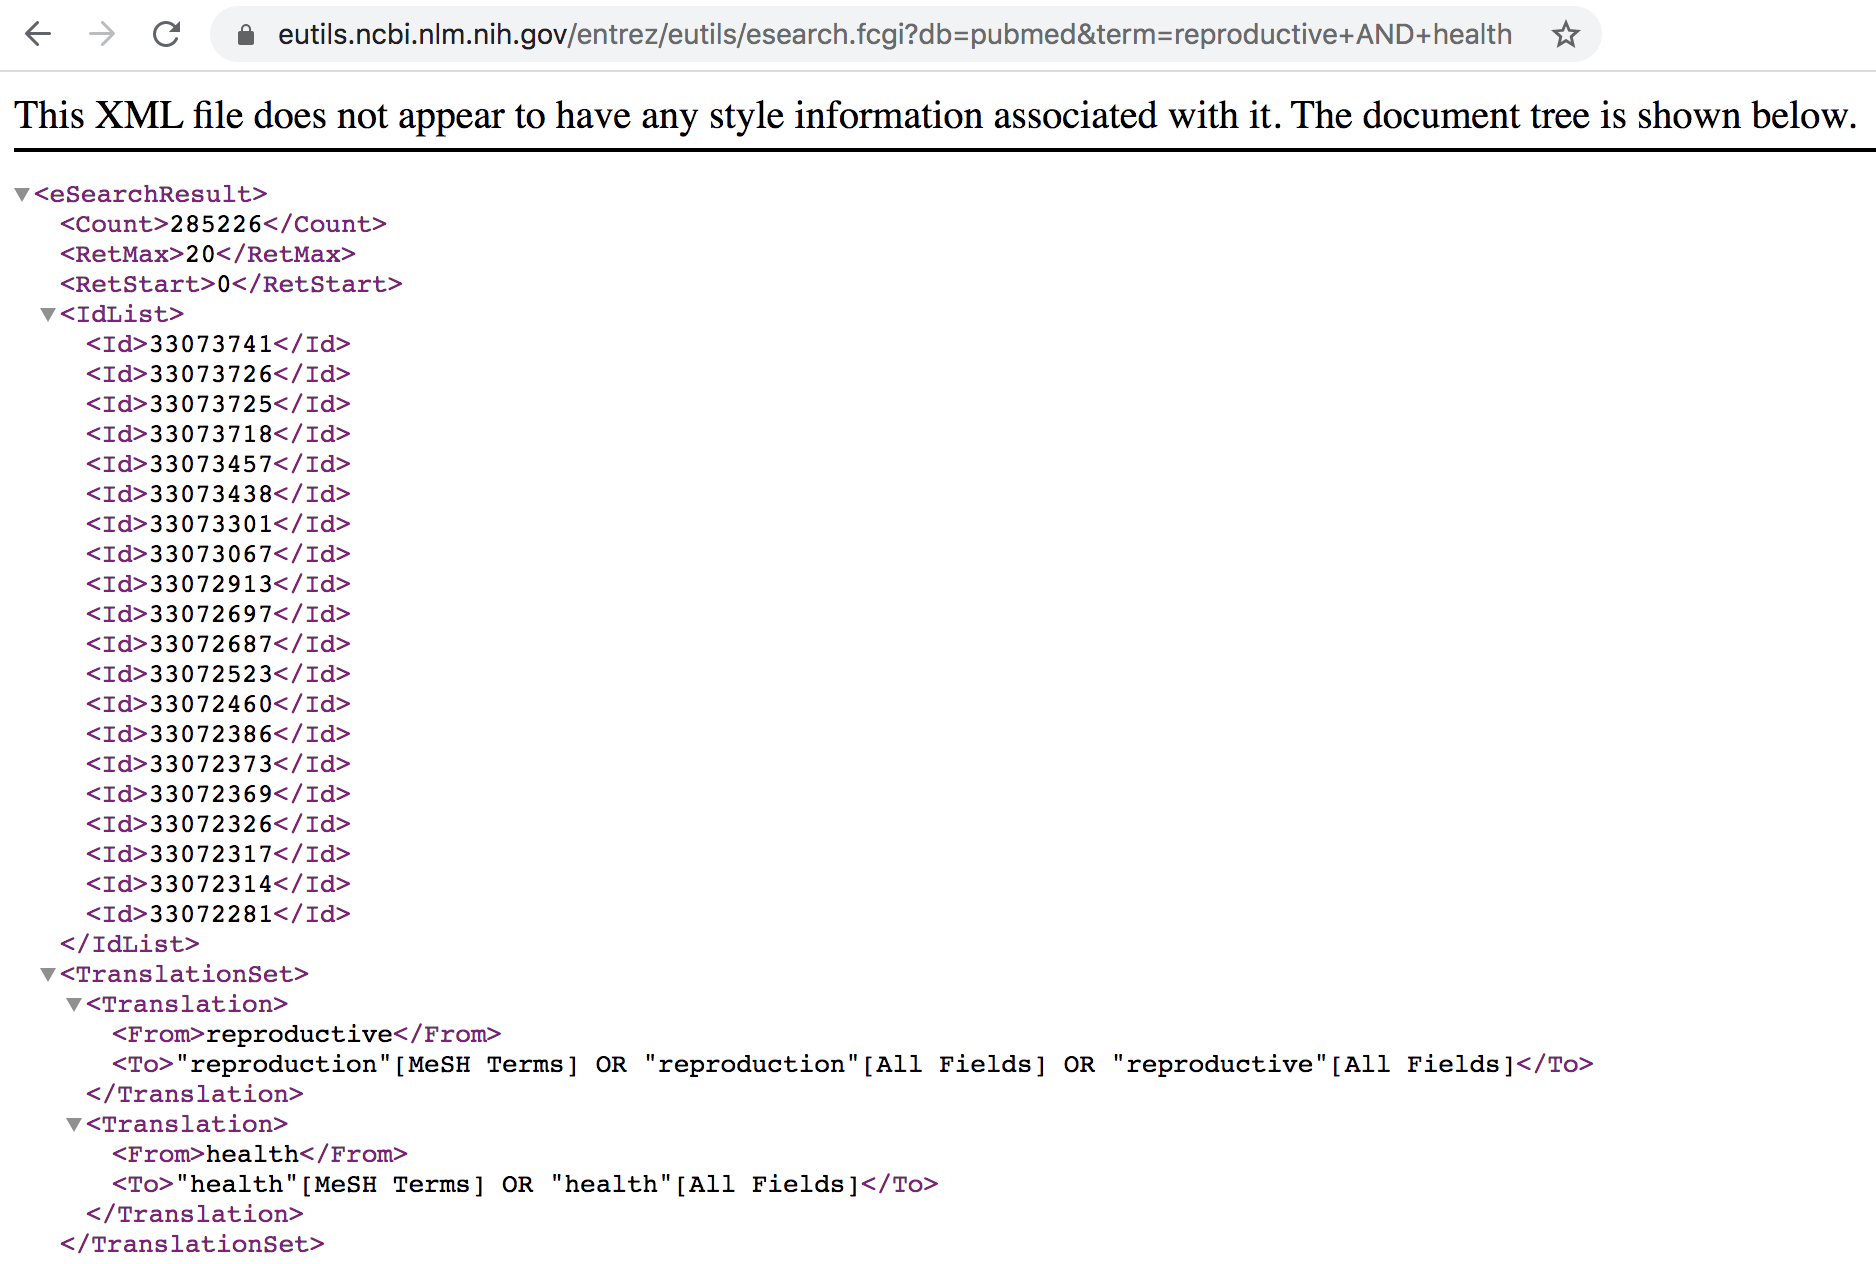
\includegraphics[width=0.8\linewidth]{images/api/pubmed-esearch} 

}

\caption{List of PubMed IDs in XML format}\label{fig:unnamed-chunk-147}
\end{figure}

\hypertarget{example-retrieving-records-with-efetch}{%
\subsubsection*{Example: Retrieving records with EFetch}\label{example-retrieving-records-with-efetch}}
\addcontentsline{toc}{subsubsection}{Example: Retrieving records with EFetch}

The \textbf{ESearch} URL retrieves a list of PMIDs---not full records. To get the
full records you need to use \textbf{EFetch}---providing the list of IDs---and the
URL would look something like this:

\begin{verbatim}
https://eutils.ncbi.nlm.nih.gov/entrez/eutils/efetch.fcgi?db=pubmed&id=33073741,33073726&retmode=abstract&rettype=text
\end{verbatim}

\begin{itemize}
\item
  \texttt{https://eutils.ncbi.nlm.nih.gov/entrez/eutils/} is the base URL
\item
  \texttt{efetch.fcgi?} indicates the E-utility (\emph{EFectch} in this case)
\item
  \texttt{db=pubmed}: indicates that the searched database is PubMed.
\item
  \texttt{id=33073741,33073726}: includes the PMIDs of the records.
\item
  \texttt{retmode=abstract}: indicates the \texttt{abstract} as the \emph{return mode}.
\item
  \texttt{rettype=text}: determines the \texttt{text} as the \emph{return type} format.
\end{itemize}

\begin{figure}

{\centering \includegraphics[width=0.8\linewidth]{images/api/pubmed-efetch} 

}

\caption{Return type in text format for abstract of specified IDs}\label{fig:unnamed-chunk-148}
\end{figure}

\hypertarget{example-retrieving-summaries-with-esummary}{%
\subsubsection*{Example: Retrieving summaries with ESummary}\label{example-retrieving-summaries-with-esummary}}
\addcontentsline{toc}{subsubsection}{Example: Retrieving summaries with ESummary}

The \textbf{ESummary} URL allows you to get the document summaries of the associated
list of PMIDs, and the URL would look something like this:

\begin{verbatim}
https://eutils.ncbi.nlm.nih.gov/entrez/eutils/esummary.fcgi?db=pubmed&id=33073741,33073726
\end{verbatim}

\begin{itemize}
\item
  \texttt{https://eutils.ncbi.nlm.nih.gov/entrez/eutils/} is the base URL
\item
  \texttt{esummary.fcgi?} indicates the E-utility (\emph{ESummary} in this case)
\item
  \texttt{db=pubmed}: indicates that the searched database is PubMed.
\item
  \texttt{id=33073741,33073726}: includes the PMIDs of the records.
\end{itemize}

The output of ESummary is a series of XML \texttt{"DocSums"} (Document Summaries), the
format of which depends on the database. Below is an example DocSum for PubMed
ID 33073741.

\begin{figure}

{\centering \includegraphics[width=0.8\linewidth]{images/api/pubmed-esummary} 

}

\caption{Summary in XML format for specified IDs}\label{fig:unnamed-chunk-149}
\end{figure}

\hypertarget{searching-pubmed-from-within-r}{%
\subsection{Searching PubMed from within R}\label{searching-pubmed-from-within-r}}

Now that you have a basic understanding of PubMed, and the E-Utilities
programs, let's see how to make requests from R.

We are going to consider a typical pipeline that involves three steps:

\begin{enumerate}
\def\labelenumi{\arabic{enumi})}
\item
  use ESearch to get a list of document IDs (default output in XML)
\item
  parse the IDs from the XML document
\item
  pass the list of IDs to either EFetch or ESummary
\end{enumerate}

\textbf{Step 1}: As a first step, we can define a character string \texttt{entrez\_url} with
the base URL, and three more strings for each of the E-utilities: \texttt{esearch},
\texttt{efetch}, and \texttt{esummary}:

\begin{Shaded}
\begin{Highlighting}[]
\CommentTok{\# base URL, and paths of associated e{-}utilities}
\NormalTok{entrez\_url }\OtherTok{\textless{}{-}} \StringTok{"https://eutils.ncbi.nlm.nih.gov/entrez/eutils/"}

\NormalTok{esearch }\OtherTok{\textless{}{-}} \StringTok{"esearch.fcgi?"}
\NormalTok{efetch }\OtherTok{\textless{}{-}} \StringTok{"efetch.fcgi?"}
\NormalTok{esummary }\OtherTok{\textless{}{-}} \StringTok{"esummary.fcgi?"}
\end{Highlighting}
\end{Shaded}

Suppose we are interested in performing a search with the following parameters:

\begin{itemize}
\item
  searching for the term \emph{BPA exposure reproductive health};
\item
  limiting our search to documents between 2018 and 2019
\item
  retaining at most the first 100 results
\end{itemize}

\textbf{Step 2}: We can assemble an R string \texttt{params\_esearch} with all the previous
ESearch query parameters:

\begin{Shaded}
\begin{Highlighting}[]
\CommentTok{\# assembling string of parameters for the query}
\NormalTok{params\_esearch }\OtherTok{\textless{}{-}} \FunctionTok{paste0}\NormalTok{(}
  \FunctionTok{c}\NormalTok{(}\StringTok{"db=pubmed"}\NormalTok{, }
    \StringTok{"term=BPA+exposure+reproductive+health"}\NormalTok{,}
    \StringTok{"mindate=2018"}\NormalTok{,}
    \StringTok{"maxdate=2019"}\NormalTok{,}
    \StringTok{"retmax=100"}\NormalTok{),}
  \AttributeTok{collapse =} \StringTok{"\&"}\NormalTok{)}

\NormalTok{params\_esearch}
\CommentTok{\#\textgreater{} [1] "db=pubmed\&term=BPA+exposure+reproductive+health\&mindate=2018\&maxdate=2019\&retmax=100"}
\end{Highlighting}
\end{Shaded}

\textbf{Step 3}: With the base URL, the \texttt{esearch} utility, and the parameters, we
assemble the required URL that we can pass to \texttt{read\_xml()}, and then use
\texttt{html\_nodes()} and \texttt{html\_text()} to extract the list of documents IDs:

\begin{Shaded}
\begin{Highlighting}[]
\CommentTok{\# assemble an esearch URL}
\NormalTok{ids\_query }\OtherTok{\textless{}{-}} \FunctionTok{paste0}\NormalTok{(entrez\_url, esearch, params\_esearch)}

\CommentTok{\# Retrieving IDs with ESearch}
\NormalTok{ids\_xml }\OtherTok{\textless{}{-}} \FunctionTok{read\_xml}\NormalTok{(ids\_query)}

\CommentTok{\# extract Ids (PMIDs)}
\NormalTok{ids }\OtherTok{\textless{}{-}} \FunctionTok{html\_text}\NormalTok{(}\FunctionTok{html\_nodes}\NormalTok{(ids\_xml, }\AttributeTok{xpath =} \StringTok{"//Id"}\NormalTok{))}
\end{Highlighting}
\end{Shaded}

The vector \texttt{ids} contains 94 retrieved document IDs, the first
5 and the last 5 five displayed below:

\begin{Shaded}
\begin{Highlighting}[]
\FunctionTok{head}\NormalTok{(ids, }\DecValTok{5}\NormalTok{)}
\CommentTok{\#\textgreater{} [1] "31771501" "31697385" "31683046" "31658598" "31648075"}

\FunctionTok{tail}\NormalTok{(ids, }\DecValTok{5}\NormalTok{)}
\CommentTok{\#\textgreater{} [1] "29549734" "29428396" "29415642" "29385186" "29317319"}
\end{Highlighting}
\end{Shaded}

\textbf{Step 4}: We can then use this list of IDs to assemble a URL for obtaining
summary information of documents---via ESummary. Notice that Esummary uses
different parameters from the ones used in ESearch. The query parameters in
this case are \texttt{db} (name of database) and \texttt{id} (list of IDs). With the base URL,
the \texttt{esummary} utility, and the parameters \texttt{params\_esummary}, we assemble the
required URL that we can pass to \texttt{read\_xml()}:

\begin{Shaded}
\begin{Highlighting}[]
\CommentTok{\# parameters for esummary}
\NormalTok{params\_esummary }\OtherTok{\textless{}{-}} \FunctionTok{paste0}\NormalTok{(}
  \StringTok{"db=pubmed\&id="}\NormalTok{, }
  \FunctionTok{paste}\NormalTok{(ids, }\AttributeTok{collapse =} \StringTok{","}\NormalTok{))}

\CommentTok{\# assemble an esummary URL}
\NormalTok{summaries\_query }\OtherTok{\textless{}{-}} \FunctionTok{paste0}\NormalTok{(entrez\_url, esummary, params\_esummary)}

\NormalTok{summaries\_xml }\OtherTok{\textless{}{-}} \FunctionTok{read\_xml}\NormalTok{(summaries\_query)}
\end{Highlighting}
\end{Shaded}

\textbf{Step 5}: To inspect the XML output we can use functions from package \texttt{"xml2"}
such as \texttt{xml\_child()} for instance. Let's take a look at the first node:

\begin{Shaded}
\begin{Highlighting}[]
\FunctionTok{xml\_child}\NormalTok{(summaries\_xml, }\AttributeTok{search =} \DecValTok{1}\NormalTok{)}
\CommentTok{\#\textgreater{} \{xml\_node\}}
\CommentTok{\#\textgreater{} \textless{}DocSum\textgreater{}}
\CommentTok{\#\textgreater{}  [1] \textless{}Id\textgreater{}31771501\textless{}/Id\textgreater{}}
\CommentTok{\#\textgreater{}  [2] \textless{}Item Name="PubDate" Type="Date"\textgreater{}2019 Oct\textless{}/Item\textgreater{}}
\CommentTok{\#\textgreater{}  [3] \textless{}Item Name="EPubDate" Type="Date"/\textgreater{}}
\CommentTok{\#\textgreater{}  [4] \textless{}Item Name="Source" Type="String"\textgreater{}Toxicol Ind Health\textless{}/Item\textgreater{}}
\CommentTok{\#\textgreater{}  [5] \textless{}Item Name="AuthorList" Type="List"\textgreater{}\textbackslash{}n  \textless{}Item Name="Author" Type="String ...}
\CommentTok{\#\textgreater{}  [6] \textless{}Item Name="LastAuthor" Type="String"\textgreater{}Sun Z\textless{}/Item\textgreater{}}
\CommentTok{\#\textgreater{}  [7] \textless{}Item Name="Title" Type="String"\textgreater{}Oral exposure to low{-}dose bisphenol A i ...}
\CommentTok{\#\textgreater{}  [8] \textless{}Item Name="Volume" Type="String"\textgreater{}35\textless{}/Item\textgreater{}}
\CommentTok{\#\textgreater{}  [9] \textless{}Item Name="Issue" Type="String"\textgreater{}10\textless{}/Item\textgreater{}}
\CommentTok{\#\textgreater{} [10] \textless{}Item Name="Pages" Type="String"\textgreater{}647{-}659\textless{}/Item\textgreater{}}
\CommentTok{\#\textgreater{} [11] \textless{}Item Name="LangList" Type="List"\textgreater{}\textbackslash{}n  \textless{}Item Name="Lang" Type="String"\textgreater{}En ...}
\CommentTok{\#\textgreater{} [12] \textless{}Item Name="NlmUniqueID" Type="String"\textgreater{}8602702\textless{}/Item\textgreater{}}
\CommentTok{\#\textgreater{} [13] \textless{}Item Name="ISSN" Type="String"\textgreater{}0748{-}2337\textless{}/Item\textgreater{}}
\CommentTok{\#\textgreater{} [14] \textless{}Item Name="ESSN" Type="String"\textgreater{}1477{-}0393\textless{}/Item\textgreater{}}
\CommentTok{\#\textgreater{} [15] \textless{}Item Name="PubTypeList" Type="List"\textgreater{}\textbackslash{}n  \textless{}Item Name="PubType" Type="Stri ...}
\CommentTok{\#\textgreater{} [16] \textless{}Item Name="RecordStatus" Type="String"\textgreater{}PubMed {-} indexed for MEDLINE\textless{}/Item\textgreater{}}
\CommentTok{\#\textgreater{} [17] \textless{}Item Name="PubStatus" Type="String"\textgreater{}ppublish\textless{}/Item\textgreater{}}
\CommentTok{\#\textgreater{} [18] \textless{}Item Name="ArticleIds" Type="List"\textgreater{}\textbackslash{}n  \textless{}Item Name="pubmed" Type="String ...}
\CommentTok{\#\textgreater{} [19] \textless{}Item Name="DOI" Type="String"\textgreater{}10.1177/0748233719885565\textless{}/Item\textgreater{}}
\CommentTok{\#\textgreater{} [20] \textless{}Item Name="History" Type="List"\textgreater{}\textbackslash{}n  \textless{}Item Name="entrez" Type="Date"\textgreater{}201 ...}
\CommentTok{\#\textgreater{} ...}
\end{Highlighting}
\end{Shaded}

The obtained summary information contains various fields such as date of
publication \texttt{PubDate}, list of authors \texttt{AuthorList}, title \texttt{Title}, starting
and ending pages \texttt{Pages}, etc.

\textbf{Step 6}: To extract all the titles, we look for the \texttt{Item} nodes with
argument \texttt{Name="Title"}. To be more precise, we can define an XPath pattern
\texttt{\textquotesingle{}//Item{[}@Name="Title"{]}\textquotesingle{}} for \texttt{xml\_nodes()}, and then extract the content
with \texttt{xml\_text()}:

\begin{Shaded}
\begin{Highlighting}[]
\NormalTok{title\_nodes }\OtherTok{\textless{}{-}} \FunctionTok{xml\_nodes}\NormalTok{(summaries\_xml, }\AttributeTok{xpath =} \StringTok{\textquotesingle{}//Item[@Name="Title"]\textquotesingle{}}\NormalTok{)}
\CommentTok{\#\textgreater{} Warning: \textasciigrave{}xml\_nodes()\textasciigrave{} was deprecated in rvest 1.0.0.}
\CommentTok{\#\textgreater{} i Please use \textasciigrave{}html\_elements()\textasciigrave{} instead.}
\CommentTok{\#\textgreater{} This warning is displayed once every 8 hours.}
\CommentTok{\#\textgreater{} Call \textasciigrave{}lifecycle::last\_lifecycle\_warnings()\textasciigrave{} to see where this warning was}
\CommentTok{\#\textgreater{} generated.}
\NormalTok{titles }\OtherTok{\textless{}{-}} \FunctionTok{xml\_text}\NormalTok{(title\_nodes)}
\FunctionTok{head}\NormalTok{(titles)}
\CommentTok{\#\textgreater{} [1] "Oral exposure to low{-}dose bisphenol A induces hyperplasia of dorsolateral prostate and upregulates EGFR expression in adult \textless{}i\textgreater{}Sprague{-}Dawley\textless{}/i\textgreater{} rats."                                   }
\CommentTok{\#\textgreater{} [2] "Juvenile Toxicity Rodent Model to Study Toxicological Effects of Bisphenol A (BPA) at Dose Levels Derived From Italian Children Biomonitoring Study."                                      }
\CommentTok{\#\textgreater{} [3] "Bisphenol F exposure impairs neurodevelopment in zebrafish larvae (Danio rerio)."                                                                                                          }
\CommentTok{\#\textgreater{} [4] "Effects of Dietary Bisphenol A on the Reproductive Function of Gilthead Sea Bream (\textless{}i\textgreater{}Sparus aurata\textless{}/i\textgreater{}) Testes."                                                                          }
\CommentTok{\#\textgreater{} [5] "Urinary bisphenol A concentration is correlated with poorer oocyte retrieval and embryo implantation outcomes in patients with tubal factor infertility undergoing in vitro fertilisation."}
\CommentTok{\#\textgreater{} [6] "In utero exposure to persistent and nonpersistent endocrine{-}disrupting chemicals and anogenital distance. A systematic review of epidemiological studies†."}
\end{Highlighting}
\end{Shaded}

Finally, we can make a wordcloud.
The code below has a series of commands to perform some text processing
(with functions from the text mining package \texttt{"tm"}) with the main terms
or words used to create the wordcloud.

\begin{Shaded}
\begin{Highlighting}[]
\CommentTok{\# title words}
\NormalTok{twords }\OtherTok{\textless{}{-}} \FunctionTok{unlist}\NormalTok{(}\FunctionTok{str\_split}\NormalTok{(titles, }\StringTok{" "}\NormalTok{))}
\NormalTok{twords }\OtherTok{\textless{}{-}} \FunctionTok{tolower}\NormalTok{(twords)}

\CommentTok{\# auxiliary vector of stop words}
\NormalTok{stop\_words }\OtherTok{\textless{}{-}} \FunctionTok{c}\NormalTok{(}
  \FunctionTok{stopwords}\NormalTok{(}\AttributeTok{kind =} \StringTok{"en"}\NormalTok{),}
  \FunctionTok{c}\NormalTok{(}\StringTok{"bisphenol"}\NormalTok{, }\StringTok{"exposure"}\NormalTok{, }\StringTok{"reproductive"}\NormalTok{, }\StringTok{"health"}\NormalTok{, }\StringTok{"bpa"}\NormalTok{)}
\NormalTok{)}

\CommentTok{\# removing unnecessary things}
\NormalTok{twords }\OtherTok{\textless{}{-}} \FunctionTok{removePunctuation}\NormalTok{(twords)}
\NormalTok{twords }\OtherTok{\textless{}{-}} \FunctionTok{removeNumbers}\NormalTok{(twords)}
\NormalTok{twords }\OtherTok{\textless{}{-}} \FunctionTok{removeWords}\NormalTok{(twords, }\FunctionTok{stopwords}\NormalTok{(}\AttributeTok{kind =} \StringTok{"en"}\NormalTok{))}
\NormalTok{twords }\OtherTok{\textless{}{-}} \FunctionTok{removeWords}\NormalTok{(twords, stop\_words)}
\NormalTok{twords }\OtherTok{\textless{}{-}}\NormalTok{ twords[twords }\SpecialCharTok{!=} \StringTok{""}\NormalTok{]}

\CommentTok{\# data frame of terms and frequencies}
\NormalTok{dat\_words }\OtherTok{\textless{}{-}} \FunctionTok{as.data.frame}\NormalTok{(}\FunctionTok{table}\NormalTok{(twords))}
\NormalTok{dat\_words }\OtherTok{\textless{}{-}}\NormalTok{ dat\_words[}\FunctionTok{order}\NormalTok{(dat\_words}\SpecialCharTok{$}\NormalTok{Freq, }\AttributeTok{decreasing =} \ConstantTok{TRUE}\NormalTok{), ]}
\FunctionTok{head}\NormalTok{(dat\_words, }\AttributeTok{n =} \DecValTok{10}\NormalTok{)}
\CommentTok{\#\textgreater{}            twords Freq}
\CommentTok{\#\textgreater{} 161       effects   18}
\CommentTok{\#\textgreater{} 500         study   10}
\CommentTok{\#\textgreater{} 519      toxicity    9}
\CommentTok{\#\textgreater{} 313          male    8}
\CommentTok{\#\textgreater{} 192             f    7}
\CommentTok{\#\textgreater{} 197        female    7}
\CommentTok{\#\textgreater{} 303        levels    7}
\CommentTok{\#\textgreater{} 464             s    7}
\CommentTok{\#\textgreater{} 173 environmental    6}
\CommentTok{\#\textgreater{} 180      estrogen    6}
\end{Highlighting}
\end{Shaded}

and then plotting a wordcloud with the function \texttt{wordcloud2()} from the package
\texttt{"wordcloud2"}:

\begin{Shaded}
\begin{Highlighting}[]
\FunctionTok{wordcloud2}\NormalTok{(dat\_words)}
\end{Highlighting}
\end{Shaded}

\begin{center}\includegraphics[width=0.7\linewidth]{images/api/wordcloud_img} \end{center}

  \bibliography{book.bib}

\end{document}
